\input{"preamble.tex"}

\addbibresource{ModuliSpaces.bib}

\let\Begin\begin
\let\End\end
\newcommand\wrapenv[1]{#1}

\makeatletter
\def\ScaleWidthIfNeeded{%
 \ifdim\Gin@nat@width>\linewidth
    \linewidth
  \else
    \Gin@nat@width
  \fi
}
\def\ScaleHeightIfNeeded{%
  \ifdim\Gin@nat@height>0.9\textheight
    0.9\textheight
  \else
    \Gin@nat@width
  \fi
}
\makeatother

\setkeys{Gin}{width=\ScaleWidthIfNeeded,height=\ScaleHeightIfNeeded,keepaspectratio}%

\title{
\rule{\linewidth}{1pt} \\
\textbf{
    Moduli Spaces
  }
    \\ {\normalsize University of Georgia, Spring 2020} \\
  \rule{\linewidth}{2pt}
}
\titlehead{
    \begin{center}
  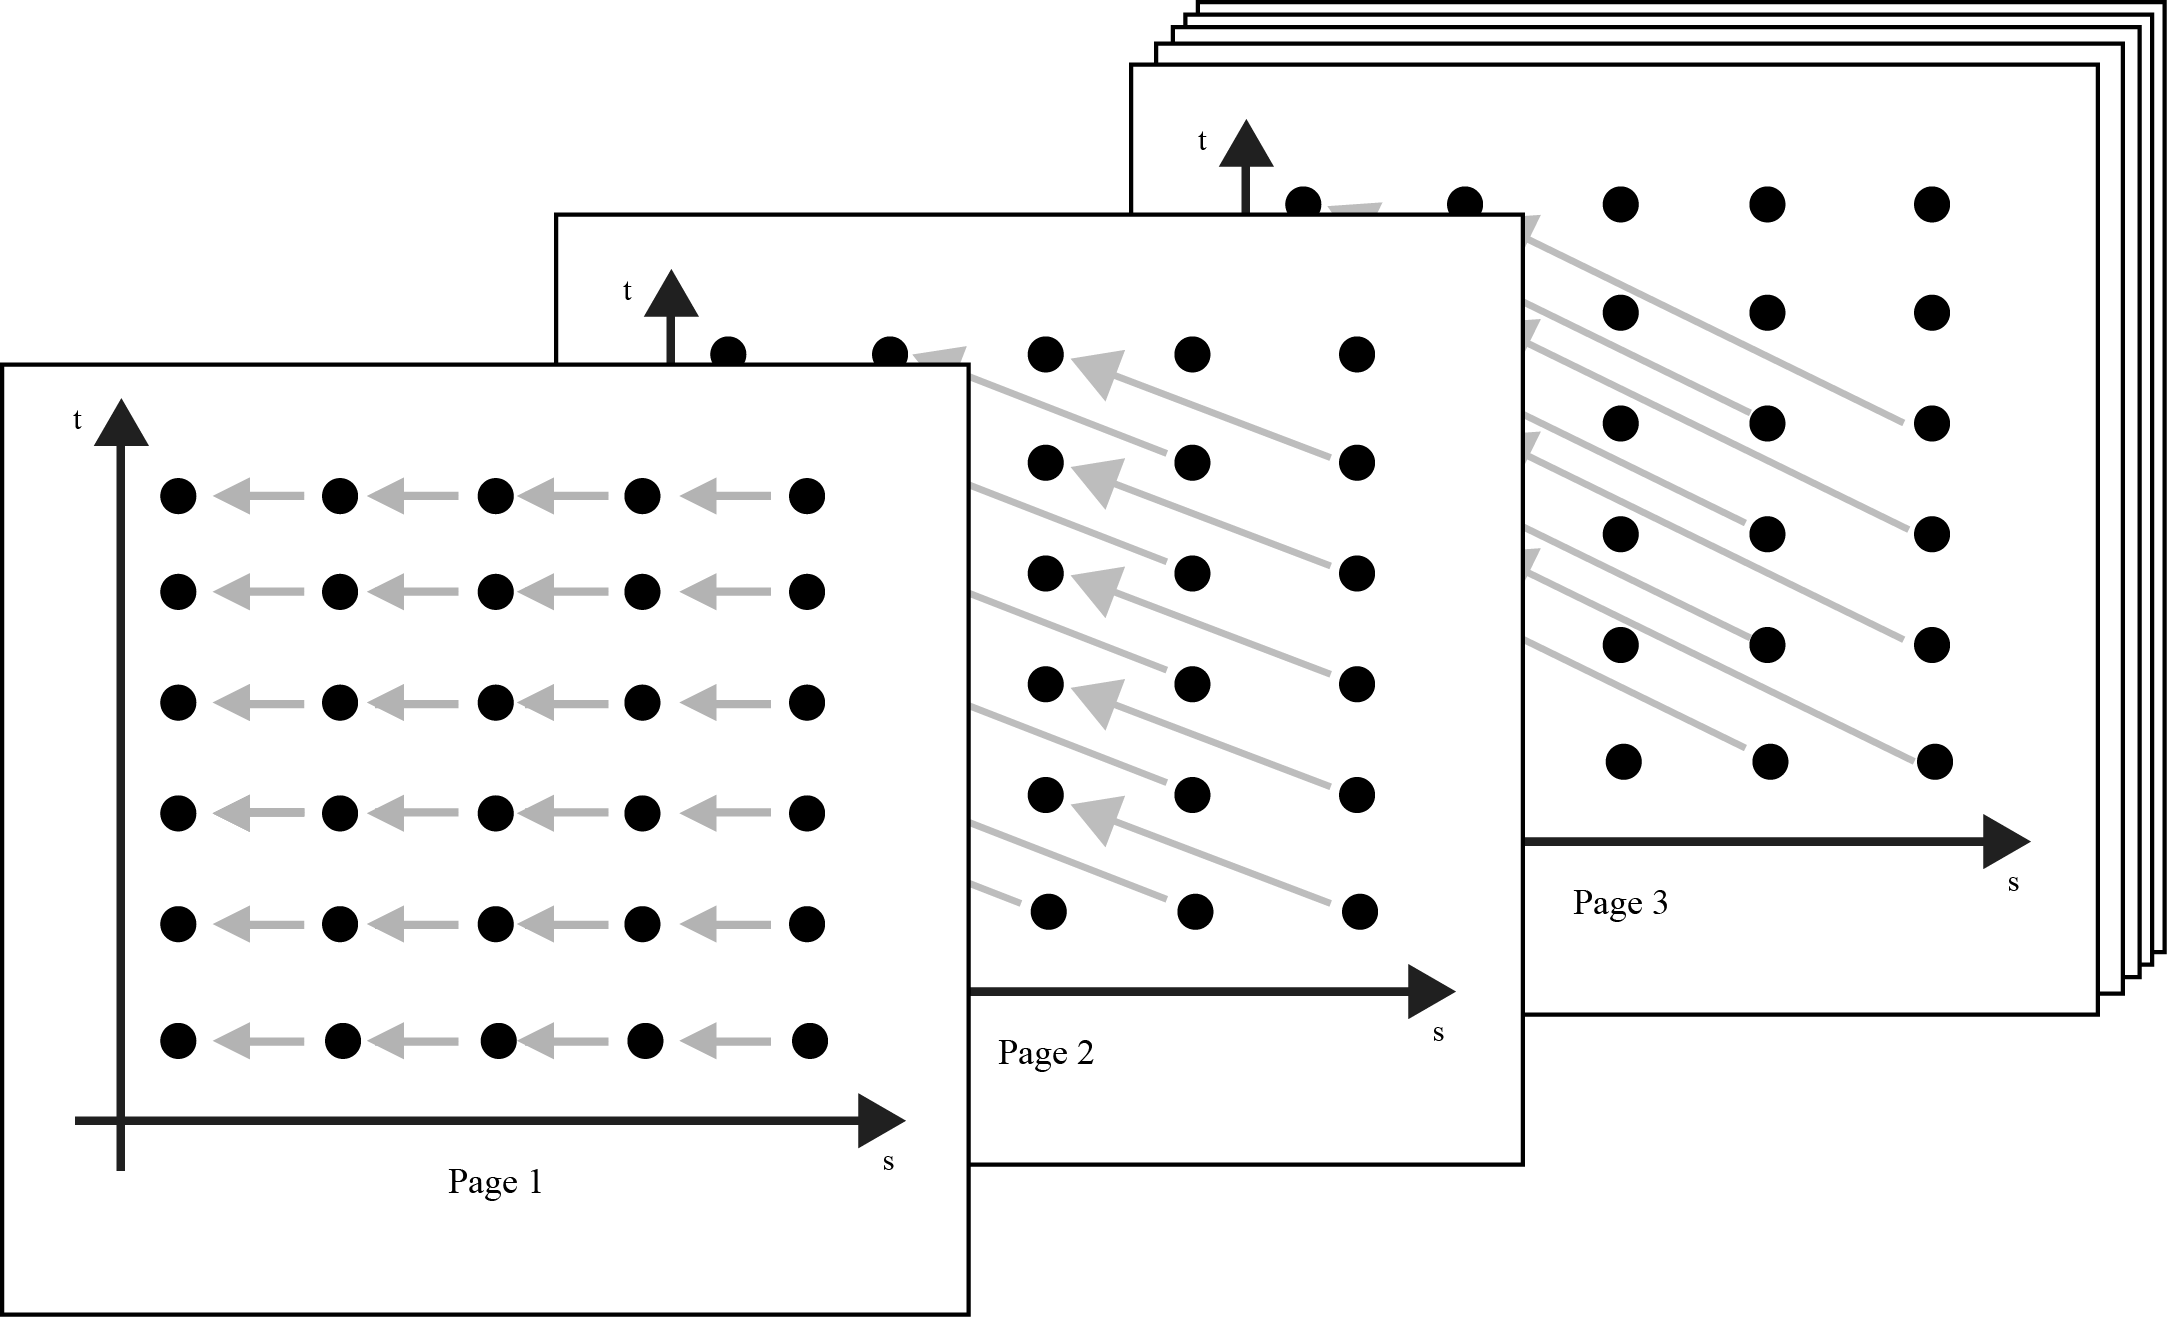
\includegraphics[width=\linewidth,height=0.45\textheight,keepaspectratio]{figures/cover.png}
  \end{center}
       \begin{minipage}{.35\linewidth}
    \begin{flushleft}
      \vspace{2em}
      {\fontsize{6pt}{2pt} \textit{Notes: These are notes live-tex'd
from a course in Moduli Spaces taught by Ben Bakker at the University of
Georgia in Spring 2020. Any errors or inaccuracies are almost certainly
my own. } } \\
    \end{flushleft}
    \end{minipage}
    \hfill
    \begin{minipage}{.65\linewidth}
    \end{minipage}
  }







\begin{document}

\date{}
\author{D. Zack Garza}
\maketitle
\begin{flushleft}
\textit{D. Zack Garza} \\
\textit{University of Georgia} \\
  \textit{\href{mailto: dzackgarza@gmail.com}{dzackgarza@gmail.com}} \\
{\tiny \textit{Last updated:} 2021-01-05 }
\end{flushleft}


\newpage

% Note: addsec only in KomaScript
\addsec{Table of Contents}
\tableofcontents
\newpage

\hypertarget{references}{%
\section{References}\label{references}}

\begin{itemize}
\item
  Course notes \autocite{bakker_8330}
\item
  General reference \autocite{hartshorne_2010}
\item
  Hilbert schemes/functors of points: \autocite{stromme},
  \autocite{hartshorne_def}.

  \begin{itemize}
  \tightlist
  \item
    Slightly more detailed: \autocite{fantechi_2005}
  \end{itemize}
\item
  Curves on surfaces: \autocite{mumford_1985}
\item
  Moduli of Curves: \autocite{harris_morrison_1998} (chatty and less
  rigorous)
\end{itemize}

\hypertarget{schemes-vs-representable-functors-thursday-january-9th}{%
\section{Schemes vs Representable Functors (Thursday January
9th)}\label{schemes-vs-representable-functors-thursday-january-9th}}

Last time: fix an \(S{\hbox{-}}\)scheme, i.e.~a scheme over \(S\). Then
there is a map
\begin{align*}
{\operatorname{Sch}}_{_{/S}} &\to {\operatorname{Fun}}( {\operatorname{Sch}}_{_{/S}}^{\operatorname{op}}, {\operatorname{Set}}) \\
x &\mapsto h_x(T) = \hom_{{\operatorname{Sch}}_{_{/S}} }(T, x)
.\end{align*}

where \(T' \xrightarrow{f} T\) is given by

\begin{align*}
h_x(f): h_x(T) &\to h_x(T') \\
\qty{ T \mapsto x } &\mapsto \text{triangles of the form}
.\end{align*}

\begin{center}
\begin{tikzcd}
T' \arrow[rr] \arrow[rdd] &               & X \\
                          &               &   \\
                          & T \arrow[ruu] &  
\end{tikzcd}
\end{center}

\hypertarget{representability}{%
\subsection{Representability}\label{representability}}

\begin{theorem}[?]

\begin{align*}\hom_{{\operatorname{Fun}}}(h_x, F) = F(x).\end{align*}

\end{theorem}

\begin{corollary}[?]

\begin{align*}\hom_{{\operatorname{Sch}}_{/S}}(x, y) \cong \hom_{{\operatorname{Fun}}}(h_x, h_y).\end{align*}

\end{corollary}

\begin{definition}[Moduli Functor]

A \textbf{moduli functor} is a map

\begin{align*}
F: ({\operatorname{Sch}}_{/S})^{\operatorname{op}}&\to {\operatorname{Set}}\\
F(x) &= \text{ "Families of something over $x$" } \\
F(f) &= \text{"Pullback"}
.\end{align*}

\end{definition}

\begin{definition}[Moduli Space]

A \textbf{moduli space} for that ``something'' appearing above is an
\(M \in \mathrm{Obj}({\operatorname{Sch}}_{/S})\) such that
\(F \cong h_M\).

\end{definition}

\begin{remark}

Now fix \(S = \operatorname{Spec}(k)\), and write \(h_m\) for the
functor of points over \(M\). Then
\begin{align*}
h_m(\operatorname{Spec}(k)) = M(\operatorname{Spec}(k)) \cong \text{families over } \operatorname{Spec}k = F(\operatorname{Spec}k)
.\end{align*}

\end{remark}

\begin{remark}

\(h_M(M) \cong F(M)\) are families over \(M\), and
\(\operatorname{id}_M \in \mathrm{Mor}_{{\operatorname{Sch}}_{/S}}(M, M) = \xi_{Univ}\)
is the universal family.

Every family is uniquely the pullback of \(\xi_{\text{Univ}}\). This
makes it much like a classifying space. For
\(T\in {\operatorname{Sch}}_{/S}\),
\begin{align*}
h_M &\xrightarrow{\cong} F \\
f\in h_M(T) &\xrightarrow{\cong} F(T) \ni \xi = F(f)(\xi_{\text{Univ}})
.\end{align*}

where \(T\xrightarrow{f} M\) and \(f = h_M(f)(\operatorname{id}_M)\).

\end{remark}

\begin{remark}

If \(M\) and \(M'\) both represent \(F\) then \(M \cong M'\) up to
unique isomorphism.

\begin{center}
\begin{tikzcd}
\xi_M              &  & \xi_{M'} \\
M \arrow[rr, "f"]  &  & M'       \\
                  &  &          \\
M' \arrow[rr, "g"] &  & M        \\
\xi_{M'}           &  & \xi_M   
\end{tikzcd}
\end{center}

which shows that \(f, g\) must be mutually inverse by using universal
properties.

\end{remark}

\begin{example}[?]

A length 2 subscheme of \({\mathbb{A}}^1_k\) (??) then
\begin{align*}
F(S) = \left\{{ V(x^2 + bx + c)}\right\} \subset {\mathbb{A}}^5
\end{align*}
where \(b, c \in {\mathcal{O}}_s(s)\), which is functorially bijective
with \(\left\{{b, c \in {\mathcal{O}}_s(s)}\right\}\) and \(F(f)\) is
pullback. Then \(F\) is representable by \({\mathbb{A}}_k^2(b, c)\) and
the universal object is given by
\begin{align*}
V(x^2 + bx + c) \subset {\mathbb{A}}^1(?) \times{\mathbb{A}}^2(b, c)
\end{align*}
where \(b, c \in k[b, c]\). Moreover, \(F'(S)\) is the set of effective
Cartier divisors in \({\mathbb{A}}_5'\) which are length 2 for every
geometric fiber. \(F''(S)\) is the set of subschemes of
\({\mathbb{A}}_5'\) which are length 2 on all geometric fibers. In both
cases, \(F(f)\) is always given by pullback.

\end{example}

Problem: \(F''\) is not a good moduli functor, as it is not
representable. Consider \(\operatorname{Spec}k[\varepsilon]\), for which
we have the following situation:

\begin{center}
\begin{tikzpicture}[scale=2.0]
\begin{axis}[
        hide axis,
    xmin=-12,
xmax=18,
    ymin=-4,
    ymax=10,
        xtick = {0},
        ytick = {0},
    disabledatascaling]

\draw[-][black][opacity=1] (axis cs:-10.0, 9) --  (axis cs:-10, -0);
\draw[-][black][opacity=1] (axis cs:-14.0, 0) --  (axis cs:-6, -0);

\draw[-][black][opacity=1] (axis cs:0.0, 9)  --  (axis cs:-0, -0);
\draw[-][black][opacity=1] (axis cs:-4.0, 0) --  (axis cs:4, -0);

\draw[-][black][opacity=1] (axis cs:10.0, 9)  --  (axis cs: 10, -0);
\draw[-][black][opacity=1] (axis cs:6.0, 0) --  (axis cs:14, -0);

\node[draw, circle, blue,  scale=0.4, fill=blue](left1) at (axis cs:-10, 6)  [anchor=center] {};
\node[right=1mm of left1,font=\tiny] {$(\varepsilon+ x  - 1)$};
\node[draw, circle, blue,  scale=0.4, fill=blue](center1) at (axis cs:0, 6)  [anchor=center] {};
\node[right=1mm of center1,font=\tiny] {$(x)(\varepsilon, x-1)$};
\node[draw, circle, blue,  scale=0.4, fill=blue](right1) at (axis cs:10, 6)  [anchor=center] {};
\node[right=1mm of right1,font=\tiny] {$(x(x-1), \varepsilon)$};

\node[draw, circle, blue,  scale=0.4, fill=blue](left2) at (axis cs:-10, 3)  [anchor=center] {};
\node[draw, circle, blue,  scale=0.4, fill=blue](center2) at (axis cs:0, 3)  [anchor=center] {};
\node[draw, circle, blue,  scale=0.4, fill=blue](right2) at (axis cs:10, 3)  [anchor=center] {};

\node[draw, circle, blue,  scale=0.4, fill=blue](left3) at (axis cs:-10, 0)  [anchor=center] {};
\node[draw, circle, blue,  scale=0.4, fill=blue](center3) at (axis cs:0, 0)  [anchor=center] {};
\node[draw, circle, blue,  scale=0.4, fill=blue](right3) at (axis cs:10, 0)  [anchor=center] {};

\draw[-][blue, very thick][opacity=0.9] (axis cs:-10.0, 6) --  (axis cs:-7, 9);
\draw[-][blue, very thick][opacity=0.9] (axis cs:-10.0, 3) --  (axis cs:-7, 3);

\draw[-][blue, very thick][opacity=0.9] (axis cs:0, 3) --  (axis cs:3, 3);
\draw[-][blue, very thick][opacity=0.9] (axis cs:0, 0) --  (axis cs:3, 0);

\draw[-][blue, very thick][opacity=0.9] (axis cs:10, 0) --  (axis cs:13, 0);
\end{axis}
\end{tikzpicture}
\end{center}

\begin{table}[H]
\centering
\begin{tabular}{l|lll}
\hline \\
$F$   & $\checkmark$ & x & x \\
$F'$  & $\checkmark$ & x &  x \\
$F''$ & $\checkmark$ & $\checkmark$ & $\checkmark$
\end{tabular}
\end{table}

\begin{center}
\begin{tikzcd}
\operatorname{Spec}k \arrow[rrr, "i", hook]                &  &  & {\operatorname{Spec}k[\varepsilon]} &  & =F'(\operatorname{Spec}k) \arrow[rd] &               \\
{F(\operatorname{Spec}k[\varepsilon])} \arrow[rrr, "F(i)"] &  &  & F(\operatorname{Spec}k) \arrow[rru] &  &                         & =F''(\operatorname{Spec}k) \\
&  &  & &  &                         &               \\
{T_p F^{', ''}}\arrow[uu, "\subset", hook]&  &  & P = V(x(x-1)) \arrow[uu, "\in", hook] & &&              
\end{tikzcd}
\end{center}

We think of \(T_p F^{', ''}\) as the tangent space at \(p\). If \(F\) is
representable, then it is actually the Zariski tangent space.

\begin{center}
\begin{tikzcd}
{M(\operatorname{Spec}k[\varepsilon])} \arrow[rr] &  & M(\operatorname{Spec}k) \\
&  & \\
T_p M \arrow[rr] \arrow[uu, "\subset", hook]&  & p \arrow[uu, "\subset", hook]         
\end{tikzcd}
\end{center}

\begin{center}
\begin{tikzcd}
&                                            & \operatorname{Spec}k \arrow[rdd, "?"] \arrow[lldd, hook] &                                     \\
&                                            &                                             &                                     \\
{\operatorname{Spec}k[\varepsilon]} \arrow[rrr] &                                            &                                             & {\operatorname{Spec}{\mathcal{O}}_{M, p} \subset M} \\
&                                            &                                             & k                                   \\
& {{\mathcal{O}}_{M, p}} \arrow[rru] \arrow[rr] &                                             & {k[\varepsilon]} \arrow[u]          \\
& {\mathfrak{m}}_p  \arrow[u, hook]                                     &                                             & (\varepsilon)  \arrow[u, hook]                       \\
& {\mathfrak{m}}_p^2 \arrow[u, hook]                                      &                                             & 0  \arrow[u, hook]                                 
\end{tikzcd}
\end{center}

Moreover, \(T_p M = ({\mathfrak{m}}_p / {\mathfrak{m}}_p^2)^\vee\), and
in particular this is a \(k{\hbox{-}}\)vector space. To see the scaling
structure, take \(\lambda \in k\).

\begin{align*}
\lambda: k[\varepsilon] & \to k[\varepsilon] \\
\varepsilon &\mapsto \lambda \varepsilon \\ \\
\lambda^*: \operatorname{Spec}(k[\varepsilon]) &\to \operatorname{Spec}(k[\varepsilon]) \\ \\
\lambda: M(\operatorname{Spec}(k[\varepsilon])) &\to M(\operatorname{Spec}(k[\varepsilon]))
.\end{align*}

\begin{center}
\begin{tikzcd}
M(\operatorname{Spec}(k[\varepsilon])) 
  \ar[r, "\lambda"]
&
M(\operatorname{Spec}(k[\varepsilon])) \\
T_pM 
  \ar[r]
  \ar[u, "\subseteq"]
& 
T_pM 
  \ar[u, "\subseteq"]
\end{tikzcd}
\end{center}

\textbf{Conclusion}: If \(F\) is representable, for each
\(p\in F(\operatorname{Spec}k)\) there exists a unique point of
\(T_p F\) that are invariant under scaling.

\begin{remark}

If
\(F, F', G \in {\operatorname{Fun}}( ({\operatorname{Sch}}_{/S})^{\operatorname{op}}, {\operatorname{Set}})\),
there exists a fiber product

\begin{center}
\begin{tikzcd}
F \times_G F' \arrow[rr, dotted] \arrow[dd, dotted] &  & F' \arrow[dd] \\
&  & \\
F \arrow[rr] &  & G            
\end{tikzcd}
\end{center}

where
\begin{align*}
(F \times_G F')(T) = F(T) \times_{G(T)} F'(T)
.\end{align*}

\end{remark}

\begin{remark}

This works with the functor of points over a fiber product of schemes
\(X \times_T Y\) for \(X, Y \to T\), where
\begin{align*}
h_{X \times_T Y}= h_X \times_{h_t} h_Y
.\end{align*}

\end{remark}

\begin{remark}

If \(F, F', G\) are representable, then so is the fiber product
\(F \times_G F'\).

\end{remark}

\begin{remark}

For any functor
\begin{align*}
F: ({\operatorname{Sch}}_{/S})^{\operatorname{op}}\to {\operatorname{Set}}
,\end{align*}
for any \(T \xrightarrow{f} S\) there is an induced functor
\begin{align*}
F_T: ({\operatorname{Sch}}_{/T}) &\to {\operatorname{Set}}\\ 
x &\mapsto F(x)
.\end{align*}

\end{remark}

\begin{remark}

\(F\) is representable by \(M_{/S}\) implies that \(F_T\) is
representable by \(M_T = M \times_S T / T\).

\end{remark}

\hypertarget{projective-space}{%
\subsection{Projective Space}\label{projective-space}}

Consider \({\mathbb{P}}^n_{\mathbb{Z}}\), i.e.~``rank 1 quotient of an
\(n+1\) dimensional free module''.

\begin{proposition}[?]

\({\mathbb{P}}^n_{/{\mathbb{Z}}}\) represents the following functor
\begin{align*}
F: {\operatorname{Sch}}^{\operatorname{op}}&\to {\operatorname{Set}}\\
S &\mapsto  \left\{{ {\mathcal{O}}_S^{n+1} \to L \to 0 }\right\} / \sim
.\end{align*}

where \(\sim\) identifies diagrams of the following form:

\begin{center}
\begin{tikzcd}
{\mathcal{O}}_s^{n+1} \arrow[dd, equal] \arrow[rr] &  & L \arrow[dd, "\cong"] \arrow[rr] &  & 0 \\
&  &                                  &  &   \\
{\mathcal{O}}_s^{n+1} \arrow[rr]                 &  & M \arrow[rr]                     &  & 0
\end{tikzcd}
\end{center}

and \(F(f)\) is given by pullbacks.

\end{proposition}

\begin{remark}

\({\mathbb{P}}^n_{/S}\) represents the following functor:
\begin{align*}
F_S: ({\operatorname{Sch}}_{/S})^{\operatorname{op}}&\to {\operatorname{Set}}\\
T &\mapsto F_S(T) =  \left\{{ {\mathcal{O}}_T^{n+1} \to L \to 0}\right\} / \sim
.\end{align*}

This gives us a cleaner way of gluing affine data into a scheme.

\end{remark}

\hypertarget{proof-of-proposition}{%
\subsubsection{Proof of Proposition}\label{proof-of-proposition}}

\begin{remark}

Note that \({\mathcal{O}}^{n+1} \to L \to 0\) is the same as giving
\(n+1\) sections \(s_1, \cdots s_n\) of \(L\), where surjectivity
ensures that they are not the zero section. So
\begin{align*}
F_i(S) = \left\{{{\mathcal{O}}_s^{n+1} \to L \to 0}\right\}/\sim
,\end{align*}
with the additional condition that \(s_i \neq 0\) at any point. There is
a natural transformation \(F_i \to F\) by forgetting the latter
condition, and is in fact a subfunctor. \footnote{\(F\leq G\) is a
  subfunctor iff \(F(s) \hookrightarrow G(s)\).}

\end{remark}

\begin{claim}

It is enough to show that each \(F_i\) and each \(F_{ij}\) are
representable, since we have natural transformations:

\begin{center}
\begin{tikzcd}
F_i  \arrow[rr]              &  & F              \\
                        &  &                \\
F_{ij} \arrow[rr] \arrow[uu] &  & F_j \arrow[uu]
\end{tikzcd}
\end{center}

and each \(F_{ij} \to F_i\) is an open embedding on the level of their
representing schemes.

\end{claim}

\begin{example}[?]

For \(n=1\), we can glue along open subschemes

\begin{center}
\begin{tikzcd}
&  & F_0 \\
F_{01} \arrow[rru] \arrow[rrd] &  &     \\
&  & F_1
\end{tikzcd}
\end{center}

For \(n=2\), we get overlaps of the following form:

\begin{center}
\begin{tikzcd}
&  &                                                                                             &                              & F_0 \arrow[rrdd] &  &   \\
&  &                                                                                             & F_{01} \arrow[rd] \arrow[ru] &                  &  &   \\
F_{012} \arrow[rr] \arrow[rrru] \arrow[rrrd] &  & F_{02} \arrow[ru] \arrow[rd] \arrow[rruu, dotted, bend left=49] \arrow[rrdd, bend right=49] &                              & F_1 \arrow[rr]   &  & F \\
&  &                                                                                             & F_{12} \arrow[ru] \arrow[rd] &                  &  &   \\
&  &                                                                                             &                              & F_2 \arrow[rruu] &  &  
\end{tikzcd}
\end{center}

This claim implies that we can glue together \(F_i\) to get a scheme
\(M\). We want to show that \(M\) represents \(F\). \(F(s)\) (LHS) is
equivalent to an open cover \(U_i\) of \(S\) and sections of
\(F_i(U_i)\) satisfying the gluing (RHS). Going from LHS to RHS isn't
difficult, since for \({\mathcal{O}}_s^{n+1} \to L \to 0\), \(U_i\) is
the locus where \(s_i \neq 0\) and by surjectivity, this gives a cover
of \(S\). The RHS to LHS comes from gluing.

\end{example}

\begin{proof}[of claim]

We have
\begin{align*}
F_i(S) = \left\{{{\mathcal{O}}_S^{n+1} \to L \cong {\mathcal{O}}_s \to 0, s_i \neq 0}\right\}
,\end{align*}
but there are no conditions on the sections other than \(s_i\).\\
So specifying \(F_i(S)\) is equivalent to specifying \(n-1\) functions
\(f_1 \cdots \widehat{f}_i \cdots f_n \in {\mathcal{O}}_S(s)\) with
\(f_k \neq 0\). We know this is representable by \({\mathbb{A}}^n\). We
also know \(F_{ij}\) is obviously the same set of sequences, where now
\(s_j \neq 0\) as well, so we need to specify
\(f_0 \cdots \widehat{f}_i \cdots f_j \cdots f_n\) with \(f_j \neq 0\).
This is representable by \({\mathbb{A}}^{n-1} \times{\mathbb{G}}_m\),
i.e.~\(\operatorname{Spec}k[x_1, \cdots, \widehat{x}_i, \cdots, x_n, x_j^{-1}]\).
Moreover, \(F_{ij} \hookrightarrow F_i\) is open.

What is the compatibility we are using to glue? For any subset
\(I \subset \left\{{0, \cdots, n}\right\}\), we can define
\begin{align*}
F_I = \left\{{{\mathcal{O}}_s^{n+1} \to L \to 0, s_i\neq 0 \text{ for } i\in I}\right\} = {\prod{i\in I}}_F F_i
,\end{align*}
and \(F_I \to F_J\) when \(I \supset J\).

\end{proof}

\hypertarget{functors-as-spaces-tuesday-january-14th}{%
\section{Functors as Spaces (Tuesday January
14th)}\label{functors-as-spaces-tuesday-january-14th}}

Last time: representability of functors, and specifically projective
space \({\mathbb{P}}_{/{\mathbb{Z}}}^n\) constructed via a functor of
points, i.e.

\begin{align*}
h_{{\mathbb{P}}^n_{/{\mathbb{Z}}} }: {\operatorname{Sch}}^{\operatorname{op}}&\to {\operatorname{Set}}\\
s &\mapsto {\mathbb{P}}^n_{/{\mathbb{Z}}}(s) = \left\{{ {\mathcal{O}}_s^{n+1} \to L \to 0}\right\}
.\end{align*}

for \(L\) a line bundle, up to isomorphisms of diagrams:

\begin{center}
\begin{tikzcd}
{\mathcal{O}}_{s}^{n+1} \arrow[dd, no head, Rightarrow] \arrow[rr] &  & L \arrow[rr] \arrow[dd, "\cong"] &  & 0 \\
&  &                                  &  &   \\
{\mathcal{O}}_{s}^{n+1} \arrow[rr]                                 &  & M \arrow[rr]                     &  & 0
\end{tikzcd}
\end{center}

That is, line bundles with \(n+1\) sections that globally generate it,
up to isomorphism. The point was that for
\(F_i \subset {\mathbb{P}}_{/{\mathbb{Z}}}^n\) where
\begin{align*}
F_i(s) = \left\{{{\mathcal{O}}_s^{n+1} \to L \to 0 {~\mathrel{\Big|}~}s_i \text{ is invertible}}\right\}
\end{align*}
are representable and can be glued together, and projective space
represents this functor.

\begin{remark}

Because projective space represents this functor, there is a universal
object:

\begin{center}
\begin{tikzcd}
  {\mathcal{O}}_{{\mathbb{P}}_{{\mathbb{Z}}}^n}^{n+1} 
  \arrow[rr] 
&  
& L \arrow[dd, equal] 
    \arrow[rr] 
&  
&
0 
\\
&  
&                                              
&  
&   
\\
&  
& {\mathcal{O}}_{{\mathbb{P}}_{{\mathbb{Z}}}^n}(1)
&  
&
\end{tikzcd}
\end{center}

and other functors are pullbacks of the universal one. (Moduli Space)

\end{remark}

\begin{exercise}[?]

Show that \({\mathbb{P}}_{/{\mathbb{Z}}}^n\) is proper over
\(\operatorname{Spec}{\mathbb{Z}}\). Use the evaluative criterion,
i.e.~there is a unique lift

\begin{center}
\begin{tikzcd}
\operatorname{Spec}k \arrow[dd] \arrow[rrr]            &  &  & {\mathbb{P}}^n_{{\mathbb{Z}}} \arrow[dd] \\
&  &  &                        \\
\operatorname{Spec}R \arrow[rrr] \arrow[rrruu, dashed] &  &  & \operatorname{Spec}{\mathbb{Z}}
\end{tikzcd}
\end{center}

\end{exercise}

\hypertarget{generalizing-open-covers}{%
\subsection{Generalizing Open Covers}\label{generalizing-open-covers}}

\begin{definition}[Equalizer]

For a category \(C\), we say a diagram \(X \to Y \rightrightarrows Z\)
is an \emph{equalizer} iff it is universal with respect to the following
property:

\begin{center}
\begin{tikzcd}
X \arrow[rr] &  & Y \arrow[rr, shift left=.5ex] \ar[rr, shift right=.5ex] &  & Z \\
&  &                                                &  &   \\
&  & S \arrow[lluu, dashed, "\exists!"] \arrow[uu] \arrow[rruu] &  &
\end{tikzcd}
\end{center}

where \(X\) is the universal object.

\end{definition}

\begin{example}[?]

For sets, \(X = \left\{{y {~\mathrel{\Big|}~}f(y) = g(y)}\right\}\) for
\(Y \xrightarrow{f, g} Z\).

\end{example}

\begin{definition}[?]

A \textbf{coequalizer} is the dual notion,

\begin{center}
\begin{tikzcd}
&  & S                       &  &                                     \\
&  &                         &  &                                     \\
Z \arrow[rruu] \arrow[rr, shift left=.5ex] \ar[rr, shift right=.5ex] &  & Y \arrow[uu] \arrow[rr] &  & X \arrow[lluu, "\exists!"', dashed]
\end{tikzcd}
\end{center}

\end{definition}

\begin{example}[?]

Take \(C = {\operatorname{Sch}}_{/S}\), \(X_{/S}\) a scheme, and
\(X_\alpha \subset X\) an open cover. We can take two fiber products,
\(X_{\alpha \beta}, X_{\beta, \alpha}\):

\begin{center}
\begin{tikzcd}
X_\alpha \arrow[rr]                   &  & X                  &  &  & X_\beta \arrow[rr]                    &  & X                   \\
&  &                    &  &  &                                       &  &                     \\
X_{\alpha\beta} \arrow[uu] \arrow[rr] &  & X_\beta \arrow[uu] &  &  & X_{\beta\alpha} \arrow[uu] \arrow[rr] &  & X_\alpha \arrow[uu]
\end{tikzcd}
\end{center}

These are canonically isomorphic.

\end{example}

In \({\operatorname{Sch}}_{/S}\), we have

\begin{center}
\begin{tikzcd}
{\coprod}_{\alpha\beta} X_{\alpha\beta}
\arrow[rr, shift left=.5ex, "f_{\alpha\beta}"]
\arrow[rr, shift right=.5ex,"g_{\alpha\beta}", swap]
&  & {\coprod}_{\alpha} X_\alpha \arrow[rr] &  & X
\end{tikzcd}
\end{center}

where
\begin{align*}
f_{\alpha\beta}: X_{\alpha\beta} &\to X_\alpha \\
g_{\alpha\beta}: X_{\alpha\beta} &\to X_\beta
;\end{align*}

form a coequalizer. Conversely, we can glue schemes. Given
\(X_\alpha \to X_{\alpha\beta}\) (schemes over open subschemes), we need
to check triple intersections:

\begin{center}
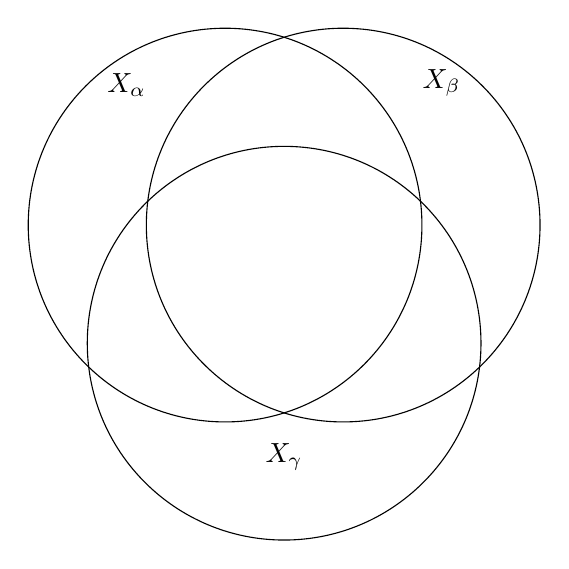
\begin{tikzpicture}[scale=0.25]
\node[draw,circle,minimum size=5cm,inner sep=0pt, label={[xshift=-1.25cm, yshift=-1.0cm] $X_\alpha$ }] at (-3,3) {};
\node[draw,circle,minimum size=5cm,inner sep=0pt, label={[xshift=1.25cm, yshift=-1.0cm] $X_\beta$ }] at (3,3) {};
\node[draw,circle,minimum size=5cm,inner sep=0pt, label={[yshift=-4.25cm] $X_\gamma$ }] at (0,-3) {};
\end{tikzpicture}
\end{center}

Then
\(\varphi_{\alpha\beta}: X_{\alpha\beta}\xrightarrow{\cong} X_{\beta\alpha}\)
must satisfy the \textbf{cocycle condition}:

\begin{definition}[Cocycle Condition]

Maps
\(\varphi_{\alpha\beta}: X_{\alpha\beta}\xrightarrow{\cong} X_{\beta\alpha}\)
satisfy the \textbf{cocycle condition} iff

\begin{enumerate}
\def\labelenumi{\arabic{enumi}.}
\item

  \begin{align*}\varphi_{\alpha\beta}^{-1}\qty{ X_{\beta\alpha} \cap X_{\beta\gamma} } = X_{\alpha\beta} \cap X_{\alpha \gamma},\end{align*}
  noting that the intersection is exactly the fiber product
  \(X_{\beta\alpha} \times_{X_\beta} X_{\beta \gamma}\).
\item
  The following diagram commutes:
\end{enumerate}

\begin{center}
\begin{tikzcd}
X_{\alpha\beta} \cap X_{\alpha\gamma} \arrow[rdd, "\varphi_{\alpha\beta}"'] \arrow[rr, "\varphi_{\alpha\gamma}"] && X_{\gamma\alpha} \cap X_{\gamma\beta} \\
&&                                             \\
& X_{\beta\alpha}\cap X_{\beta\gamma} \arrow[ruu, "\varphi_{\beta\gamma}"'] &
\end{tikzcd}
\end{center}

\end{definition}

Then there exists a scheme \(X_{/S}\) such that
\({\coprod}_{\alpha\beta} X_{\alpha\beta} \rightrightarrows {\coprod}X_\alpha \to X\)
is a coequalizer; this is the gluing.

Subfunctors satisfy a patching property because morphisms to schemes are
locally determined. Thus representable functors (e.g.~functors of
points) have to be (Zariski) sheaves.

\begin{definition}[Zariski Sheaf]

A functor
\(F: ({\operatorname{Sch}}_{/S})^{\operatorname{op}}\to {\operatorname{Set}}\)
is a \textbf{Zariski sheaf} iff for any scheme \(T_{/S}\) and any open
cover \(T_\alpha\), the following is an equalizer:
\begin{align*}
F(T) \to \prod F(T_\alpha) \rightrightarrows \prod_{\alpha\beta} F(T_{\alpha\beta})
\end{align*}
where the maps are given by restrictions.

\end{definition}

\begin{example}[?]

Any representable functor is a Zariski sheaf precisely because the
gluing is a coequalizer. Thus if you take the cover
\begin{align*}
{\coprod}_{\alpha\beta} T_{\alpha\beta} \to {\coprod}_{\alpha}T_\alpha \to T
,\end{align*}
since giving a local map to \(X\) that agrees on intersections if enough
to specify a map from \(T\to X\).

Thus any functor represented by a scheme automatically satisfies the
sheaf axioms.

\end{example}

\begin{definition}[Subfunctors and Open/Closed Functors]

Suppose we have a morphism \(F' \to F\) in the category
\({\operatorname{Fun}}({\operatorname{Sch}}_{/S}, {\operatorname{Set}})\).

\begin{itemize}
\item
  This is a \textbf{subfunctor} if \(\iota(T)\) is injective for all
  \(T_{/S}\).
\item
  \(\iota\) is \textbf{open/closed/locally closed} iff for any scheme
  \(T_{/S}\) and any section \(\xi \in F(T)\) over \(T\), then there is
  an open/closed/locally closed set \(U\subset T\) such that for all
  maps of schemes \(T' \xrightarrow{f} T\), we can take the pullback
  \(f^* \xi\) and \(f^*\xi \in F'(T')\) iff \(f\) factors through \(U\).
\end{itemize}

\end{definition}

\begin{remark}

This says that we can test if pullbacks are contained in a subfunctors
by checking factorization. This is the same as asking if the subfunctor
\(F'\), which maps to \(F\) (noting a section is the same as a map to
the functor of points), and since \(T\to F\) and \(F' \to F\), we can
form the fiber product \(F' \times_F T\):

\begin{center}
\begin{tikzcd}
F' \ar[r] & F \\
& \\
F' \times_F T \ar[r, "g"] \ar[uu] & T \ar[uu, "\xi" swap]
\end{tikzcd}
\end{center}

and \(F' \times_F T \cong U\). Note: this is almost tautological! Thus
\(F' \to F\) is open/closed/locally closed iff \(F' \times_F T\) is
representable and \(g\) is open/closed/locally closed. I.e. base change
is representable.

\end{remark}

\begin{exercise}[?]

\envlist

\begin{enumerate}
\def\labelenumi{\arabic{enumi}.}
\item
  If \(F' \to F\) is open/closed/locally closed and \(F\) is
  representable, then \(F'\) is representable as an open/closed/locally
  closed subscheme
\item
  If \(F\) is representable, then open/etc subschemes yield open/etc
  subfunctors
\end{enumerate}

\end{exercise}

\begin{slogan}

Treat functors as spaces.

\end{slogan}

We have a definition of open, so now we'll define coverings.

\begin{definition}[Open Covers]

A collection of open subfunctors \(F_\alpha \subset F\) is an
\textbf{open cover} iff for any \(T_{/S}\) and any section
\(\xi \in F(T)\), i.e.~\(\xi: T\to F\), the \(T_\alpha\) in the
following diagram are an open cover of \(T\):

\begin{center}
\begin{tikzcd}
F_\alpha \ar[r] & F \\
& \\
T_\alpha \ar[uu] \ar[r] & T \ar[uu, "\xi" swap]
\end{tikzcd}
\end{center}

\end{definition}

\begin{example}[?]

Given
\begin{align*}
F(s) = \left\{{{\mathcal{O}}_s^{n+1} \to L \to 0}\right\}
\end{align*}
and \(F_i(s)\) given by those where \(s_i \neq 0\) everywhere, the
\(F_i \to F\) are an open cover. Because the sections generate
everything, taking the \(T_i\) yields an open cover.

\end{example}

\hypertarget{results-about-zariski-sheaves}{%
\subsection{Results About Zariski
Sheaves}\label{results-about-zariski-sheaves}}

\begin{proposition}[?]

A Zariski sheaf
\(F: ({\operatorname{Sch}}_{/S})^{\operatorname{op}}\to {\operatorname{Set}}\)
with a representable open cover is representable.

\end{proposition}

\begin{proof}[?]

Let \(F_\alpha \subset F\) be an open cover, say each \(F_\alpha\) is
representable by \(x_\alpha\). Form the fiber product
\(F_{\alpha\beta} = F_\alpha \times_F F_\beta\). Then \(x_\beta\) yields
a section (plus some openness condition?), so
\(F_{\alpha\beta} = x_{\alpha\beta}\) representable. Because
\(F_\alpha \subset F\), the \(F_{\alpha\beta} \to F_\alpha\) have the
correct gluing maps.

This follows from Yoneda (schemes embed into functors), and we get maps
\(x_{\alpha\beta} \to x_\alpha\) satisfying the gluing conditions. Call
the gluing scheme \(x\); we'll show that \(x\) represents \(F\). First
produce a map \(x\to F\) from the sheaf axioms. We have a map
\(\xi \in \prod_\alpha F(x_\alpha)\), and because we can pullback, we
get a unique element \(\xi \in F(X)\) coming from the diagram
\begin{align*}
F(x) \to \prod F(x_\alpha) \rightrightarrows \prod_{\alpha\beta} F(x_{\alpha\beta})
.\end{align*}

\end{proof}

\begin{lemma}[?]

If \(E \to F\) is a map of functors and \(E, F\) are Zariski sheaves,
where there are open covers \(E_\alpha \to E, F_\alpha \to F\) with
commutative diagrams

\begin{center}
\begin{tikzcd}
E \ar[r] & F \\
  & \\
E_\alpha \ar[uu] \ar[r, "\cong"] & F_\alpha \ar[uu]
\end{tikzcd}
\end{center}

(i.e.~these are isomorphisms locally), then the map is an isomorphism.

\end{lemma}

With the following diagram, we're done by the lemma:

\begin{center}
\begin{tikzcd}
X \ar[r] & F \\
  & \\
X_\alpha \ar[uu] \ar[r, "\cong"] & F_\alpha \ar[uu]
\end{tikzcd}
\end{center}

\begin{example}[?]

For \(S\) and \(E\) a locally free coherent \({\mathcal{O}}_s\) module,
\begin{align*}
{\mathbb{P}}E(T) = \left\{{f^* E \to L \to 0}\right\} / \sim
\end{align*}
is a generalization of projectivization, then \(S\) admits a cover
\(U_i\) trivializing \(E\). Then the restriction
\(F_i \to {\mathbb{P}}E\) were \(F_i(T)\) is the above set if \(f\)
factors through \(U_i\) and empty otherwise. On \(U_i\),
\(E \cong {\mathcal{O}}_{U_i}^{n_i}\), so \(F_i\) is representable by
\({\mathbb{P}}_{U_i}^{n_i - 1}\) by the proposition. Note that this is
clearly a sheaf.

\end{example}

\begin{example}[?]

For \(E\) locally free over \(S\) of rank \(n\), take \(r<n\) and
consider the functor
\begin{align*}
{\operatorname{Gr}}(k, E)(T) = \left\{{f^*E \to Q \to 0}\right\} /\sim
\end{align*}
(a Grassmannian) where \(Q\) is locally free of rank \(k\).

\end{example}

\begin{exercise}[?]

\envlist

\begin{enumerate}
\def\labelenumi{\arabic{enumi}.}
\item
  Show that this is representable
\item
  For the Plucker embedding
  \begin{align*}
  {\operatorname{Gr}}(k, E) \to {\mathbb{P}}\wedge^k E
  ,\end{align*}
  a section over \(T\) is given by \(f^*E \to Q \to 0\) corresponding to
  \begin{align*}
  \wedge^k f^*E \to \wedge^k Q \to 0
  ,\end{align*}
  noting that the left-most term is \(f^* \wedge^k E\). Show that this
  is a closed subfunctor.
\end{enumerate}

\begin{quote}
That it's a functor is clear, that it's closed is not.
\end{quote}

\end{exercise}

Take \(S = \operatorname{Spec}k\), then \(E\) is a \(k{\hbox{-}}\)vector
space \(V\), then sections of the Grassmannian are quotients of
\(V \otimes{\mathcal{O}}\) that are free of rank \(n\). Take the
subfunctor \(G_w \subset {\operatorname{Gr}}(k, V)\) where
\begin{align*}
G_w(T) = \left\{{{\mathcal{O}}_T \otimes V \to Q \to 0}\right\} \text{ with } Q \cong {\mathcal{O}}_t\otimes W \subset {\mathcal{O}}_t \otimes V
.\end{align*}
If we have a splitting \(V = W \oplus U\), then
\(G_W = {\mathbb{A}}(\hom(U, W))\). If you show it's closed, it follows
that it's proper by the exercise at the beginning.

\begin{quote}
Thursday: Define the Hilbert functor, show it's representable. The
Hilbert scheme functor gives e.g.~for \({\mathbb{P}}^n\) of all flat
families of subschemes.
\end{quote}

\hypertarget{thursday-january-16th}{%
\section{Thursday January 16th}\label{thursday-january-16th}}

\hypertarget{subfunctors}{%
\subsection{Subfunctors}\label{subfunctors}}

\begin{definition}[Open Functors]

A functor
\(F' \subset F: ({\operatorname{Sch}}_{/S})^{\operatorname{op}}\to {\operatorname{Set}}\)
is \textbf{open} iff for all \(T \xrightarrow{\xi} F\) where \(T = h_T\)
and \(\xi \in F(T)\).

\end{definition}

We can take fiber products:

\begin{center}
\begin{tikzcd}
F' \ar[r] & F \\
 & \\
\parbox{3cm}{\centering $F' \times_F T$ \\ Representable} \ar[r, "\text{Open}"] \ar[uu] & T \ar[uu]
\end{tikzcd}
\end{center}

So we can think of ``inclusion in \(F\)'' as being an \emph{open
condition}: for all \(T_{/S}\) and \(\xi \in F(T)\), there exists an
open \(U \subset T\) such that for all covers \(f: T' \to T\), we have
\begin{align*}
F(f)(\xi) = f^*(\xi) \in F'(T')
\end{align*}
iff \(f\) factors through \(U\).

Suppose \(U \subset T\) in \({\operatorname{Sch}}/T\), we then have
\begin{align*}
h_{U/T}(T') = \begin{cases}
\emptyset & T' \to T \text{ doesn't factor } \\
{\{\operatorname{pt}\}}& \text{otherwise}
\end{cases}
.\end{align*}

which follows because the literal statement is
\(h_{U/T}(T') = \hom_T(T', U)\). By the definition of the fiber product,
\begin{align*}
(F' \times_F T)(T') = \left\{{ (a,b) \in F'(T) \times T(T) {~\mathrel{\Big|}~}\xi(b) = \iota(a) \text{ in  } F(T)}\right\}
,\end{align*}
where \(F' \xrightarrow{\iota} F\) and \(T \xrightarrow{\xi} F\). So
note that the RHS diagram here is exactly given by pullbacks, since we
identify sections of \(F/T'\) as sections of \(F\) over \(T/T'\) (?).

\begin{center}
\begin{tikzcd}
F' \ar[r, "\iota"] & F \\
 & & \\
F' \times_F T \ar[uu] \ar[r] & T\ar[uu, "\xi"] \\
 & & \\
& & T'
\ar[uuuul, "f\circ \xi", bend right]
\ar[uul, "f"]
\end{tikzcd}
\end{center}

We can thus identify
\begin{align*}
(F' \times_F T)(T') = h_{U_{/S}}(T')
,\end{align*}
and so for \(U \subset T\) in \({\operatorname{Sch}}_{/S}\) we have
\(h_{U_{/S}} \subset h_{T_{/S}}\) is the functor of maps that factor
through \(U\). We just identify \(h_{U_{/S}}(T') = \hom_S(T', U)\) and
\(h_{T_{/S}}(T') = \hom_S(T', T)\).

\begin{example}[?]

\({\mathbb{G}}_m, {\mathbb{G}}_a\). The scheme/functor
\({\mathbb{G}}_a\) represents giving a global function,
\({\mathbb{G}}_m\) represents giving an invertible function.

\begin{center}
\begin{tikzcd}
{\mathbb{G}}_m \ar[r] & {\mathbb{G}}_a \\
& \\
T'
\arrow[uur, phantom, "\scalebox{1.5}{$\llcorner$}" , very near start, color=black]
\ar[uu] \ar[r] & T \ar[uu, "f \in {\mathcal{O}}_T(T)", swap]
\end{tikzcd}
\end{center}

where \(T' = \left\{{f\neq 0}\right\}\) and \({\mathcal{O}}_T(T)\) are
global functions.

\end{example}

\hypertarget{actual-geometry-hilbert-schemes}{%
\subsection{Actual Geometry: Hilbert
Schemes}\label{actual-geometry-hilbert-schemes}}

\begin{quote}
The best moduli space!
\end{quote}

\begin{warnings}

Unless otherwise stated, assume all schemes are Noetherian.

\end{warnings}

We want to parameterize families of subschemes over a fixed object. Fix
\(k\) a field, \(X_{/k}\) a scheme; we'll parameterize subschemes of
\(X\).

\begin{definition}[The Hilbert Functor]

The \textbf{Hilbert functor} is given by
\begin{align*}
\operatorname{Hilb}_{X_{/S}}: ({\operatorname{Sch}}_{/S})^{op} \to {\operatorname{Set}}
\end{align*}
which sends \(T\) to closed subschemes \(Z \subset X \times_S T \to T\)
which are flat over \(T\).

\end{definition}

Here \textbf{flatness} will replace the Cartier condition:

\begin{definition}[Flatness]

For \(X \xrightarrow{f} Y\) and \({\mathbb{F}}\) a coherent sheaf on
\(X\), \(f\) is \textbf{flat} over \(Y\) iff for all \(x\in X\) the
stalk \(F_x\) is a flat \({\mathcal{O}}_{y, f(x)}{\hbox{-}}\)module.

\end{definition}

\begin{remark}

Note that \(f\) is flat if \({\mathcal{O}}_x\) is. Flatness corresponds
to varying continuously. Note that everything works out if we only play
with finite covers.

\end{remark}

\begin{remark}

If \(X_{/k}\) is projective, so \(X \subset {\mathbb{P}}^n_k\), we have
line bundles \({\mathcal{O}}_x(1) = {\mathcal{O}}(1)\). For any sheaf
\(F\) over \(X\), there is a Hilbert polynomial
\(P_F(n) = \chi(F(n)) \in {\mathbb{Z}}[n]\), i.e.~we twist by
\({\mathcal{O}}(1)\) \(n\) times. The cohomology of \(F\) isn't changed
by the pushforward into \({\mathbb{P}}_n\) since it's a closed
embedding, and so
\begin{align*}
\chi(X, F) = \chi({\mathbb{P}}^n, i_* F) = \sum (-1)^i \dim_k H^i({\mathbb{P}}^n, i_* F(n))
.\end{align*}

\end{remark}

\begin{fact}

For \(n \gg 0\), \(\dim_k H^0 = \dim M_n\), the \(n\)th graded piece of
\(M\), which is a graded module over the homogeneous coordinate ring
whose \(i_*F = \tilde M\).

\end{fact}

In general, for \(L\) ample of \(X\) and \(F\) coherent on \(X\), we can
define a \textbf{Hilbert polynomial},
\begin{align*}
P_F(n) = \chi(F\otimes L^n)
.\end{align*}

This is an invariant of a polarized projective variety, and in
particular subschemes. Over irreducible bases, flatness corresponds to
this invariant being constant.

\begin{proposition}[?]

For \(f:X\to S\) projective, i.e.~there is a factorization:

\begin{center}
\begin{tikzcd}
X \arrow[ddr, "f"] \arrow[rr, hook] & & {\mathbb{P}}^n \times S \ni {\mathcal{O}}(1) \ar[ddl] \\
& & \\
& S &
\end{tikzcd}
\end{center}

If \(S\) is reduced, irreducible, locally Noetherian, then \(f\) is flat
\(\iff\) \(P_{{\mathcal{O}}_{x_s}}\) is constant for all \(s\in S\).

\end{proposition}

\begin{remark}

To be more precise, look at the base change to \(X_1\), and the pullback
of the fiber? \({\mathcal{O}}\mathrel{\Big|}_{x_i}\)? Note that we're
not using the word ``integral'' here! \(S\) is flat \(\iff\) the Hilbert
polynomial over the fibers are constant.

\end{remark}

\begin{example}[?]

The zero-dimensional subschemes \(Z \in {\mathbb{P}}^n_k\), then \(P_Z\)
is the length of \(Z\), i.e.~\(\dim_k({\mathcal{O}}_Z)\), and
\begin{align*}
P_Z(n) = \chi({\mathcal{O}}_Z \otimes{\mathcal{O}}(n)) = \chi({\mathcal{O}}_Z) = \dim_k H^0(Z; {\mathcal{O}}_Z) = \dim_k {\mathcal{O}}_Z(Z)
.\end{align*}

For two closed points in \({\mathbb{P}}^2\), \(P_Z = 2\). Consider the
affine chart \({\mathbb{A}}^2 \subset {\mathbb{P}}^2\), which is given
by
\begin{align*}
\operatorname{Spec}k[x, y]/(y, x^2) \cong k[x]/(x^2)
\end{align*}
and \(P_Z = 2\). I.e. in flat families, it has to record how the tangent
directions come together.

\end{example}

\begin{example}[?]

Consider the flat family \(xy = 1\) (flat because it's an open
embedding) over \(k[x]\), here we have points running off to infinity.

\end{example}

\begin{proposition}[Modified Characterization of Flatness for Sheaves]

A sheaf \(F\) is flat iff \(P_{F_S}\) is constant.

\end{proposition}

\hypertarget{proof-that-flat-sheaves-have-constant-hilbert-polynomials}{%
\subsection{Proof That Flat Sheaves Have Constant Hilbert
Polynomials}\label{proof-that-flat-sheaves-have-constant-hilbert-polynomials}}

Assume \(S = \operatorname{Spec}A\) for \(A\) a local Noetherian domain.

\begin{lemma}[?]

For \(F\) a coherent sheaf on \(X_{/A}\) is flat, we can take the
cohomology via global sections \(H^0(X; F(n))\). This is an
\(A{\hbox{-}}\)module, and is a free \(A{\hbox{-}}\)module for
\(n\gg 0\).

\end{lemma}

\begin{proof}[of lemma]

Assumed \(X\) was projective, so just take \(X = {\mathbb{P}}_A^n\) and
let \(F\) be the pushforward. There is a correspondence sending \(F\) to
its ring of homogeneous sections constructed by taking the sheaf
associated to the graded module\\

\begin{align*}
\sum_{n\gg0} H^0( {\mathbb{P}}_A^m; F(n) )
=
\bigoplus_{n \gg 0} H^0({\mathbb{P}}_A^m; F(n))
\end{align*}
and taking the associated sheaf (\(Y \mapsto \tilde Y\), as per
Hartshorne's notation) which is free, and thus \(F\) is free.
\footnote{See tilde construction in Hartshorne, essentially amounts to
  localizing free tings.}

Conversely, take an affine cover \(U_i\) of \(X\). We can compute the
cohomology using Čech cohomology, i.e.~taking the Čech resolution. We
can also assume \(H^i({\mathbb{P}}^m; F(n)) = 0\) for \(n \gg 0\), and
the Čech complex vanishes in high enough degree. But then there is an
exact sequence
\begin{align*}
0 \to H^0({\mathbb{P}}^m; F(n)) \to \mathcal C^0( \underline{U}; F(n) ) \to \cdots \to C^m( \underline{U}; F(n) ) \to 0
.\end{align*}
Assuming \(F\) is flat, and using the fact that flatness is a 2 out of 3
property, the images of these maps are all flat by induction from the
right. Finally, local Noetherian and finitely generated flat implies
free.

\end{proof}

By the lemma, we want to show \(H^0({\mathbb{P}}^m; F(n))\) is free for
\(n\gg 0\) iff the Hilbert polynomials on the fibers \(P_{F_S}\) are all
constant.

\begin{claim}[1]

It suffices to show that for each point \(s\in \operatorname{Spec}A\),
we have
\begin{align*}
H^0(X_s; F_S(n)) = H^0(X; F(n)) \otimes k(S)
\end{align*}
for \(k(S)\) the residue field, for \(n\gg 0\).

\end{claim}

\begin{claim}[2]

\(P_{F_S}\) measures the rank of the LHS.

\end{claim}

\begin{proof}[of claim 2]

\(\implies\): The dimension of RHS is constant, whereas the LHS equals
\(P_{F_S}(n)\).

\(\impliedby\): If the dimension of the RHS is constant, so the LHS is
free.

\end{proof}

For a f.g. module over a local ring, testing if localization at closed
point and generic point have the same rank. For \(M\) a finitely
generated module over \(A\), we find that
\begin{align*}
0 \to A^n \to M \to Q
\end{align*}
is surjective after tensoring with \(\mathrm{Frac}(A)\), and tensoring
with \(k(S)\) for a closed point, if \(\dim A^n = \dim M\) then
\(Q = 0\).

\begin{proof}[of claim 1]

By localizing, we can assume \(s\) is a closed point. Since \(A\) is
Noetherian, its ideal is f.g. and we have
\begin{align*}
A^m \to A \to k(S) \to 0
.\end{align*}
We can tensor with \(F\) (viewed as restricting to fiber) to obtain
\begin{align*}
F(n)^m \to F(n) \to F_S(n) \to 0
.\end{align*}
Because \(F\) is flat, this is still exact. We can take
\(H^*(x, {\,\cdot\,})\), and for \(n\gg 0\) only \(H^0\) survives. This
is the same as tensoring with \(H^0(x, F(n))\).

\end{proof}

\begin{definition}[Hilbert Polynomial Subfunctor]

Given a polynomial \(P \in {\mathbb{Z}}[n]\) for \(X_{/S}\) projective,
we define a subfunctor by picking only those with Hilbert polynomial
\(p\) fiberwise as
\(\operatorname{Hilb}^P_{X_{/S}} \subset \operatorname{Hilb}_{X_{/S}}\).
This is given by \(Z \subset X \times_S T\) with \(P_{Z} = P\).

\end{definition}

\begin{theorem}[Grothendieck]

If \(S\) is Noetherian and \(X_{/S}\) projective, then
\(\operatorname{Hilb}_{X_{/S}}^P\) is representable by a projective
\(S{\hbox{-}}\)scheme.

\begin{quote}
See \textbf{cycle spaces} in analytic geometry.
\end{quote}

\end{theorem}

\hypertarget{hilbert-polynomials-thursday-january-23}{%
\section{Hilbert Polynomials (Thursday January
23)}\label{hilbert-polynomials-thursday-january-23}}

Some facts about the Hilbert polynomial:

\begin{enumerate}
\def\labelenumi{\arabic{enumi}.}
\item
  For a subscheme \(Z \subset {\mathbb{P}}_k^n\) with
  \(\deg P_z = \dim Z = n\), then
  \begin{align*}
    p_z(t) = \deg z \frac{t^n}{n!} + O(t^{n-1})
    .\end{align*}
\item
  We have \(p_z(t) = \chi({\mathcal{O}}_z(t))\), consider the sequence
  \begin{align*}
    0 \to I_z(t) \to {\mathcal{O}}_{{\mathbb{P}}^n}^{(t)} \to {\mathcal{O}}_z^{(t)} \to 0
    ,\end{align*}
  then \(\chi(I_z(t)) = \dim H^0( {\mathbb{P}}^n, J_z(t) )\) for
  \(t \gg 0\), and \(p_z(0)\) is the Euler characteristic of
  \({\mathcal{O}}_Z\).
\end{enumerate}

\begin{remark}

Keywords to look up here: Serre vanishing, Riemann-Roch, ideal sheaf.

\end{remark}

\begin{example}[The twisted cubic]

\begin{center}
\begin{tikzpicture}[x=0.75pt,y=0.75pt,yscale=-1,xscale=1, scale=0.6, every node/.style={scale=0.6}]

\node (myfirstpic) at (325,200) {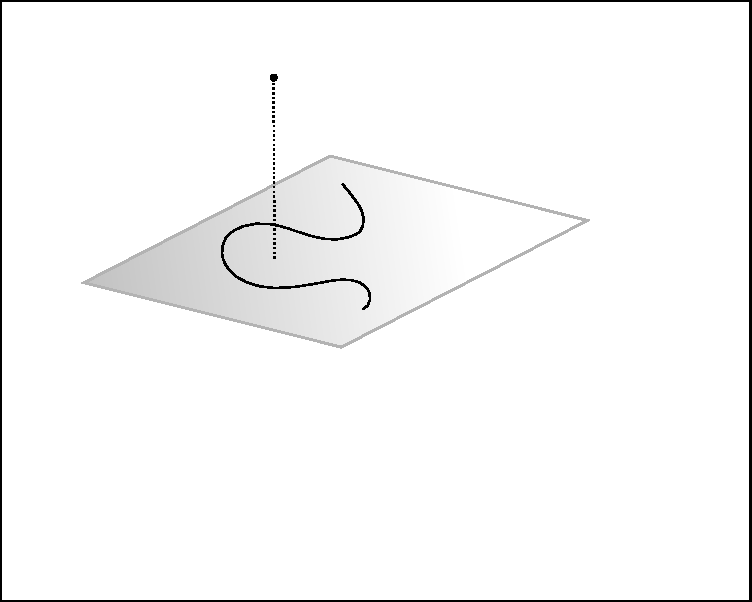
\includegraphics{/home/zack/SparkleShare/github.com/Notes/Class_Notes/2020/Spring/Moduli Spaces/sections/figures/2021-01-03_17-27}};
\node[scale=2.0] at (400, 180) {$C$};
\node[scale=2.0] at (200, 0) {${\mathbb{P}}^3$};


\draw[very thick, blue] (-50,400) -- (-50,100);
\draw[thick] (-50-20,400) -- (-50+20,400);
\draw[thick] (-50-20,100) -- (-50+20,100);
\node[scale=2.0] at (-25, 100-20) {${\mathbb{P}}^1$};

\draw [thick, right hook-latex ] (-50+20, 200) -- (150, 200);
\node[scale=2.0] at (50, 180) {$\iota$};

\end{tikzpicture}
\end{center}

Then
\begin{align*}
p_C(t) = (\deg C)t + \chi({\mathcal{O}}_{{\mathbb{P}}^1}) = 3t + 1
.\end{align*}

\end{example}

\hypertarget{hypersurfaces}{%
\subsubsection{Hypersurfaces}\label{hypersurfaces}}

Recall that length 2 subschemes of \({\mathbb{P}}^1\) are the same as
specifying quadratics that cut them out, each such
\(Z \subset {\mathbb{P}}^1\) satisfies \(Z = V(f)\) where \(\deg f = d\)
and \(f\) is homogeneous. So we'll be looking at
\({\mathbb{P}}H^0({\mathbb{P}}^n_k, {\mathcal{O}}(d))^\vee\), and the
guess would be that this is \(\operatorname{Hilb}_{{\mathbb{P}}^n_k}\)
Resolve the structure sheaf

\begin{align*}
0 \to {\mathcal{O}}_{{\mathbb{P}}^n}(-d) \to {\mathcal{O}}_{{\mathbb{P}}^n}(t) \to {\mathcal{O}}_D(t) \to 0
.\end{align*}
so we can twist to obtain
\begin{align*}
0 \to {\mathcal{O}}_{{\mathbb{P}}^n}(t-d) \to {\mathcal{O}}_{{\mathbb{P}}^n}(t) \to {\mathcal{O}}_D(t) \to 0
.\end{align*}
Then
\begin{align*}
\chi({\mathcal{O}}_D(t)) = \chi({\mathcal{O}}_{{\mathbb{P}}^n}(t)) - \chi({\mathcal{O}}_{{\mathbb{P}}^n}(t-d))
,\end{align*}
which is
\begin{align*}
{n+t \choose n} - {n+t-d \choose n} = \frac{dt^{n-1}}{(n-1)!} + O(t^{n-2})
.\end{align*}

\begin{lemma}[?]

Anything with the Hilbert polynomial of a degree \(d\) hypersurface is
in fact a degree \(d\) hypersurface.

\end{lemma}

We want to write a morphism of functors
\begin{align*}
\operatorname{Hilb}_{{\mathbb{P}}^n_k}^{P_{n, d}} \to {\mathbb{P}}H^0 ({\mathbb{P}}^n, {\mathcal{O}}(d) )^\vee
.\end{align*}
which sends flat families to families of equations cutting them out.
Want
\begin{align*}
Z \subset {\mathbb{P}}^n \times S \to {\mathcal{O}}_s \otimes H^0( {\mathbb{P}}^n, {\mathcal{O}}(d) )^\vee\to L \to 0
.\end{align*}
This happens iff
\begin{align*}
0 \to L^\vee\to {\mathcal{O}}_s \otimes H^0({\mathbb{P}}^n, {\mathcal{O}}(d))
\end{align*}
with torsion-free quotient. Note that we use \(L^\vee\) instead of
\({\mathcal{O}}_s\) because of scaling. We have
\begin{align*}
0 \to I_z &\to {\mathcal{O}}_{{\mathbb{P}}^n \times S} \to {\mathcal{O}}_z \to 0 \\
0 \to I_z(d) &\to {\mathcal{O}}_{{\mathbb{P}}^n \times S}(d) \to {\mathcal{O}}_z(d) \to 0 \quad\text{by twisting}
.\end{align*}
We then consider \(\pi_s: {\mathbb{P}}^n \times S \to S\), and apply the
pushforward to the above sequence. Notie that it is not right-exact:

\begin{center}
\begin{tikzcd}
  0 
  \ar[r]  
& \pi_{s*} I_z(d) 
  \ar[r] 
& \pi_{s*} {\mathcal{O}}_{{\mathbb{P}}^n \times S}(d) 
  \ar[r] 
& \pi_{s*} {\mathcal{O}}_z(d) 
  \ar[r] 
&  0 
\\
& & & & 
\\
  \ar[uu, equal]0 
  \ar[r] 
& {\mathcal{O}}_s \otimes H^0({\mathbb{P}}^n, {\mathcal{O}}(d)) 
  \ar[uu, equal]L^\vee= 
  \ar[uu, equal]
  \ar[r] 
& 
  \ar[uu, equal]\text{locally free} 
  \ar[r] 
& 0
\ar[uu, equal]
\end{tikzcd}
\end{center}

\todo[inline]{Note: above diagram may be off horizontally?}

This equality follows from flatness, cohomology, and base change. In
particular, we need the following:

\begin{fact}

The scheme-theoretic fibers, given by \(H^0({\mathbb{P}}^n, I_z(d))\)
and \(H^0({\mathbb{P}}^n, {\mathcal{O}}_z(d))\), are all the same
dimension.

\end{fact}

Using

\begin{enumerate}
\def\labelenumi{\arabic{enumi}.}
\item
  Cohomology and base change, i.e.~for \(X \xrightarrow{f} Y\) a map of
  Noetherian schemes (or just finite-type) and \(F\) a sheaf on \(X\)
  which is flat over \(Y\), there is a natural map (not usually an
  isomorphism)
  \begin{align*}
  R^i f_* f \otimes k(y) \to H^i(x_y,  {\left.{{F}} \right|_{{x_y}} } )
  ,\end{align*}
  but is an isomorphism if
  \(\dim H^i(x_y, {\left.{{F}} \right|_{{x_y}} } )\) is constant, in
  which case \(R^i f_* f\) is locally free.
\item
  If \(Z \subset {\mathbb{P}}^n_k\) is a degree \(d\) hypersurface, then
  independently we know
  \begin{align*}
    \dim H^0({\mathbb{P}}^n, I_z(d)) = 1 \text{ and } \dim H^0({\mathbb{P}}^n, {\mathcal{O}}_z(d)) = {d+n \choose n} - 1
    .\end{align*}
\end{enumerate}

To get a map going backwards, we take the universal degree 2 polynomial
and form
\begin{align*}
V(a_{00} x_0^2 + a_{11} x_1^2 + a_{12}x_2^2 + a_{01}x_0 x_1 + a_{02} x_0 x_2 + a_{12} x_1 x_2) \subset {\mathbb{P}}^2 \times{\mathbb{P}}^5
.\end{align*}

\hypertarget{example-twisted-cubics}{%
\subsubsection{Example: Twisted Cubics}\label{example-twisted-cubics}}

Consider a map \({\mathbb{P}}^1 \to {\mathbb{P}}^3\) obtained by taking
a basis of a homogeneous cubic polynomial. The canonical example is
\begin{align*}
(x, y) \to (x^3, x^2y, xy^2, y^3)
.\end{align*}
Then
\begin{align*}
P_C(t) = 3t + 1
\end{align*}
and \(\operatorname{Hilb}_{{\mathbb{P}}_k^3}^{3t+1}\) has a component
with generic point a twisted cubic, and another component with points a
curve disjoint union a point, and the overlap are nodal curves with a
``fat'' 3-dimensional point:

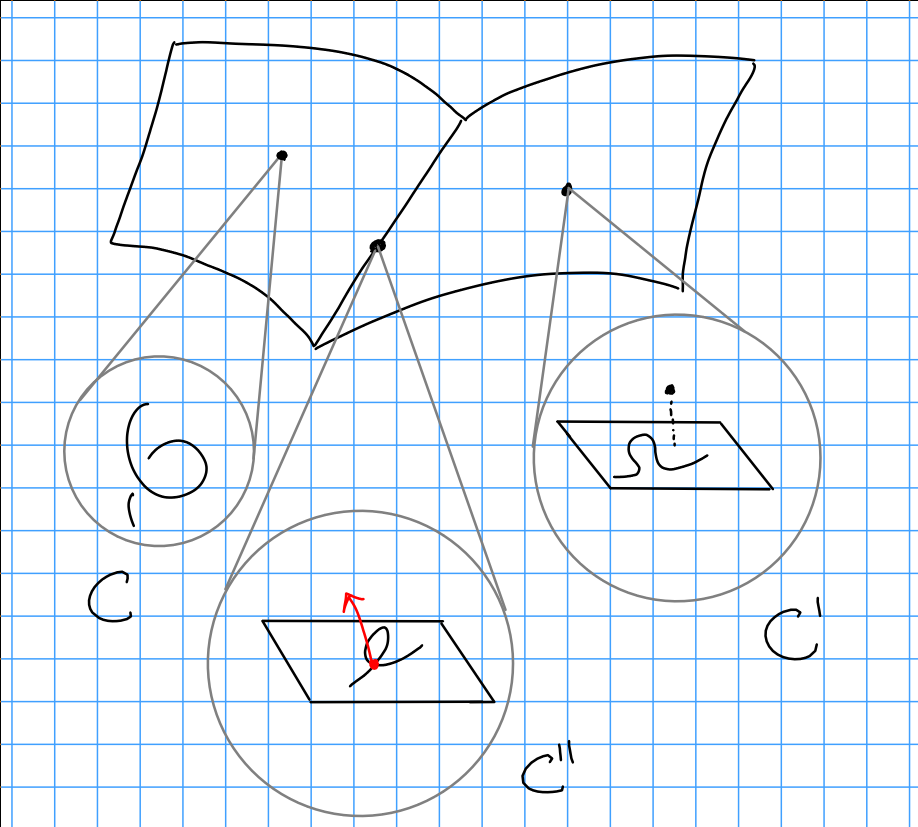
\includegraphics{figures/2020-01-23-13:20.png}\\

Then \(P_{C'} = 1 + \tilde P\), the Hilbert polynomial of just the base
without the disjoint point, so this equals
\(1 + P_{2, 3} = 1 + (3t + 0) = 3t +1\). For \(P_{C''}\), we take the
sequence
\begin{align*}
0 \to k \to {\mathcal{O}}_{C''} \to {\mathcal{O}}_{C'' \text{reduced}} \to 0
,\end{align*}
so
\begin{align*}
P_{C''} = 1 + P_{C'' \text{red}} = 3t+1
.\end{align*}

\begin{remark}

Note that flat families \emph{must} have the same (constant) Hilbert
polynomial.

\end{remark}

Note that we can get paths in this space from \(C\to C''\) and
\(C'\to C''\) by collapsing a twisted cubic onto a plane, and sending a
disjoint point crashing into the node on a nodal cubic. We're mapping
\({\mathbb{P}}^1 \to {\mathbb{P}}^3\), and there is a natural action of
\(\operatorname{PGL}(4) \curvearrowright{\mathbb{P}}^3\), so we get a
map
\begin{align*}
\operatorname{PGL}(4) \times{\mathbb{P}}^3 \to {\mathbb{P}}^3
.\end{align*}

Let \(c\in {\mathbb{P}}^3\) and let \({\mathcal{C}}\) be the preimage.
This induces (?) a map
\begin{align*}
\operatorname{PGL}(4) \to \operatorname{Hilb}_{{\mathbb{P}}^3}^{3t+1}
\end{align*}
where the fiber over \([C]\) in the latter is
\(\operatorname{PGL}(2) = {\operatorname{Aut}}({\mathbb{P}}^1)\). By
dimension counting, we find that the dimension of the twisted cubic
component is \(15 - 3 = 12\). The 15 in the other component comes from
3-dim choices of plane, 3-dim choices of a disjoint point, and
\begin{align*}
{\mathbb{P}}H^0({\mathbb{P}}^2, {\mathcal{O}}(3))^\vee\cong {\mathbb{P}}^9
,\end{align*}
yielding 15 dimensions. To show that these are actually different
components, we use Zariski tangent spaces. Let \(T_1\) be the tangent
space of the twisted cubic component, then
\begin{align*}
\dim T_1 \operatorname{Hilb}_{{\mathbb{P}}_k^3}^{3t+1} = 12
,\end{align*}
and similarly the dimension of the tangent space over the \(C'\)
component is 15.

\begin{fact}

Let \(A\) be Noetherian and local, then the dimension of the Zariski
tangent space, \(\dim {\mathfrak{m}}/{\mathfrak{m}}^2 \geq \dim A\), the
Krull dimension. If this is an equality, then \(A\) is regular.

\end{fact}

\begin{slogan}

Dimensions of tangent spaces give an upper bound.

\end{slogan}

\begin{proposition}[?]

If \(X_{/k}\) is projective and \(P\) is a Hilbert polynomial, then
\([Z] \in \operatorname{Hilb}_{X_{/k}}^P\), i.e.~a closed subscheme of
\(X\) with Hilbert polynomial \(p\) (note there's an ample bundle
floating around) then the tangent space is
\(\hom_{{\mathcal{O}}_x}(I_z, {\mathcal{O}}_z)\).

\end{proposition}

\hypertarget{hilbert-schemes-of-hypersurfaces-tuesday-january-28th}{%
\section{Hilbert Schemes of Hypersurfaces (Tuesday January
28th)}\label{hilbert-schemes-of-hypersurfaces-tuesday-january-28th}}

Last time: Twisted cubics, given by
\(\operatorname{Hilb}_{{\mathbb{P}}^3_k}^{3t+1}\).

\begin{center}
\begin{tikzpicture}
\node (node_one) at (0,0) {
  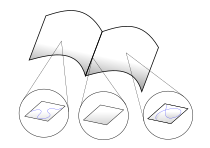
\includegraphics{/home/zack/SparkleShare/github.com/Notes/Class_Notes/2020/Spring/Moduli Spaces/sections/figures/2021-01-03_21-29}
  };

\node (a) at (0, -4) {$?$};

\node (a) at (-4.5, 3.9) {$A$};
\filldraw[blue](-4.45, 3.4) circle (0.1);

\node (a) at (2.44, 2.4) {$B$};
\filldraw[blue](2.04, 2.2) circle (0.1);

\node (a) at (-1.8, 1.85) {$C$};
\filldraw[red](-1.38, 1.85) circle (0.1);

\node (a) at (-4., 7) {$12$};
\node (a) at (3., 5.5) {$15$};
\end{tikzpicture}
\end{center}

\begin{quote}
Components of the Scheme of Cubic Curves.
\end{quote}

We got lower (?) bounds on the dimension by constructing families, but
want an exact dimension. The following will be a key fact:

\begin{proposition}[?]

Let \(Z\subset X\) be a closed \(k{\hbox{-}}\)dimensional subspace. For
\([z] \in \operatorname{Hilb}_{X_{_{/k}}}^P(k)\), we have an
identification of the Zariski tangent space
\begin{align*}
T_{[z]} \operatorname{Hilb}_{X_{_{/k}} }^P = \hom_{{\mathcal{O}}_X}(I_z, {\mathcal{O}}_Z)
\end{align*}

\end{proposition}

Say
\begin{align*}
F: ({\operatorname{Sch}}_{_{_{/k}}})^{\operatorname{op}}\to {\operatorname{Set}}
\end{align*}
is a functor and let \(x\in F(k)\). There is an inclusion
\(i: \operatorname{Spec}k \hookrightarrow\operatorname{Spec}k[\varepsilon]\)
and an induced map

\begin{align*}
F(\operatorname{Spec}k [\varepsilon]) &\xrightarrow{i^*} F(\operatorname{Spec}k) \\
T_x F \coloneqq(i^*)^{-1}(x) &\mapsto x
\end{align*}
So if \(F\) is represented by a scheme \(H_{/k}\), then\\
\begin{align*}
T_x h_J = T_x H = ({\mathfrak{m}}_x / {\mathfrak{m}}_x^2)^\vee\,\,\text{over } k
\end{align*}
Will need a criterion for flatness later, esp.~for Artinian thickenings.

\begin{lemma}[?]

Assume \(A'\) is a Noetherian ring and \(0 \to J \to A' \to A \to 0\)
with \(J^2 = 0\). Assume we have \(X'_{/ \operatorname{Spec}A'}\), and a
coherent sheaf \(F'\) on \(X'\), where \(X'\) is Noetherian. Then \(F'\)
is flat over \(A'\) iff

\begin{enumerate}
\def\labelenumi{\arabic{enumi}.}
\tightlist
\item
  \(F\) is flat
\item
  \(0 \to F\otimes_A J \to F'\) is exact.
\end{enumerate}

\begin{center}
\begin{tikzcd}
F 
&
F'
\\
X \coloneqq\operatorname{Spec}A' \times_{\operatorname{Spec}A} X
  \ar[r] 
  \ar[d]
& 
X'
  \ar[d] 
\\
\operatorname{Spec}A
  \arrow[ur, phantom, "\scalebox{1.5}{$\ulcorner$}" , very near start, color=black]
  \ar[r]
& 
\operatorname{Spec}A'
\end{tikzcd}
\end{center}

\end{lemma}

\hypertarget{sketch-proof-of-lemma}{%
\subsubsection{Sketch Proof of Lemma}\label{sketch-proof-of-lemma}}

Take the first exact sequence and tensor with \(F'\) (which is
right-exact), then \(J \otimes_{A'} F' = J \otimes_A\) canonically. This
follows because \(J = J \otimes_{A'} A\), and there is an isomorphism
\(J \otimes_{A'} A' \to J \otimes_{A'} A\). And
\(F = F' \otimes_{A'} A\) is a pullback of \(F'\). If flat, then
tensoring is exact. Note that both conditions in the lemma are necessary
since pullbacks of flats are flat by (1), and (2) gives the flatness
condition.

\begin{definition}[Flat Modules]

Recall that for a module over a Noetherian ring, \(M/A\), \(M\) is
\textbf{flat} over \(A\) iff
\begin{align*}
\operatorname{Tor}_1^A(M, A/p) = 0 && 
\text{ for all primes } p
.\end{align*}

\end{definition}

\begin{remark}

Reason: Tor commutes with direct limits, so \(M\) is flat iff

\begin{align*}
\operatorname{Tor}_1^A(M, N) = 0
&& \text{for all finitely generated } N
.\end{align*}

\end{remark}

Since \(A\) is Noetherian, \(N\) has a finite filtration \(N^\cdot\)
where \(N_i / N_{i+1} \cong A/p_i\). Use the fact that every ideal is
contained in a prime ideal. Take \(x\in N\), this yields a map
\(A\to N\) which factors through \(A/I\). If we make such a filtration
on \(A/I\), then we can quotient \(N\) by \(\operatorname{im}f\) where
\(f: A/I \to N\). Continuing inductively, the resulting filtration must
stabilize. So we can assume \(N = A/I\). Then \(I\) is contained in a
maximal.

\begin{exercise}[?]

Finish proof. See Aatiyah Macdonald.

\end{exercise}

\hypertarget{proof-of-proposition-1}{%
\subsubsection{Proof of Proposition}\label{proof-of-proposition-1}}

\begin{proof}[of proposition, given lemma]

So it's enough to show that \(\operatorname{Tor}_1^{A'}(F', A'/p') = 0\)
for all primes \(p' \subset A'\).

\begin{observation}

Since \(J\) is nilpotent, \(J \subset p'\).

\end{observation}

\hypertarget{consequences-of-proof}{%
\subsection{Consequences of Proof}\label{consequences-of-proof}}

Let \(p = p'/J\), this is a prime ideal. We have an exact diagram by
taking quotients:

\begin{center}
\begin{tikzcd}
             &  &              &  & 0 \arrow[dd]             &  & 0 \arrow[dd]            &  &   \\
             &  &              &  &                          &  &                         &  &   \\
0 \arrow[rr] &  & J \arrow[rr] &  & p' \arrow[rr] \arrow[dd] &  & p \arrow[rr] \arrow[dd] &  & 0 \\
             &  &              &  &                          &  &                         &  &   \\
0 \arrow[rr] &  & J \arrow[rr] &  & A' \arrow[rr] \arrow[dd] &  & A \arrow[rr] \arrow[dd] &  & 0 \\
             &  &              &  &                          &  &                         &  &   \\
             &  &              &  & A'/p' \arrow[dd]         &  & A/p \arrow[dd]          &  &   \\
             &  &              &  &                          &  &                         &  &   \\
             &  &              &  & 0                        &  & 0                       &  &
\end{tikzcd}
\end{center}

So we can tensor with \(F'\) everywhere, and get a map from kernels to
cokernels using the snake lemma:

\begin{center}
\begin{tikzcd}
             &  &                                                                  &  & 0 \arrow[dd]                                     &  & {\operatorname{Tor}(A, F) = 0} \arrow[dd]             &  &   \\
             &  &                                                                  &  &                                                  &  &                                         &  &   \\
             &  & 0 \arrow[rr, "\text{snake}"] \arrow[dd]                          &  & {\operatorname{Tor}_1^{A_1}(A'/p', F')} \arrow[dd]             &  & {\operatorname{Tor}_1^{A_1}(A/p, F')} \arrow[dd]      &  &   \\
             &  &                                                                  &  &                                                  &  &                                         &  &   \\
0 \arrow[rr] &  & J \otimes_{A'} F' \arrow[rr, "\text{by commuting square}", hook] &  & p' \otimes_{A'} F' \arrow[rr] \arrow[dd]         &  & p \otimes_{A'} F' \arrow[rr] \arrow[dd] &  & 0 \\
             &  &                                                                  &  &                                                  &  &                                         &  &   \\
0 \arrow[rr] &  & J \otimes_{A'} F' \arrow[rr, "\text{by (2)}"', hook]             &  & A' \otimes_{A'} F' \arrow[rr] \arrow[dd]         &  & A \otimes_{A'} F' \arrow[rr] \arrow[dd] &  & 0 \\
             &  &                                                                  &  &                                                  &  &                                         &  &   \\
             &  & 0 \arrow[rr, "\text{snake}"]                                     &  & A'/p' \otimes_{A'} F' \arrow[dd] \arrow[rr, "="] &  & A/p \otimes_{A'} F' \arrow[dd]          &  &   \\
             &  &                                                                  &  &                                                  &  &                                         &  &   \\
             &  &                                                                  &  & 0                                                &  & 0                                       &  &
\end{tikzcd}
\end{center}

Then by (1), we have
\begin{align*}
\operatorname{Tor}_1^{A'}(A'/p', F') = \operatorname{Tor}_1^{A'}(A/p, F') = 0
.\end{align*}

\end{proof}

We will just need this for \(A' = k[\varepsilon]\) and \(A=k\).

\begin{proposition}[?]

\begin{align*}
T_z \operatorname{Hilb}_{X_{_{/k}}} = \hom_{{\mathcal{O}}_x}(I_z, {\mathcal{O}}_z)
.\end{align*}

\end{proposition}

\begin{proof}[?]

Again we have
\(T_z \operatorname{Hilb}_{X_{_{/k}}} \subset \operatorname{Hilb}_{X_{_{/k}}}(k[\varepsilon])\),
and is given by
\begin{align*}
\left\{{Z' \subset X \times_{\operatorname{Spec}k} \operatorname{Spec}k[\varepsilon] 
{~\mathrel{\Big|}~}Z' \text{ is flat}_{/k[\varepsilon]},\,\, Z' \times_{\operatorname{Spec}k[\varepsilon]}\operatorname{Spec}k = Z}\right\}
.\end{align*}

We have an exact diagram:

\begin{center}
\begin{tikzcd}
              &  & 0 \arrow[r]  & I_{Z'} \arrow[r]           & {{\mathcal{O}}_{X[\varepsilon]}} \arrow[r]                               & {\mathcal{O}}_{Z'} \arrow[r]           & 0  \\
0 \arrow[d]         &  &              & {} \arrow[d]               & {} \arrow[d]                                            & {} \arrow[d]                 &    \\
k \arrow[d]         &  & {} \arrow[r] & I_Z \arrow[r] \arrow[d]    & {\mathcal{O}}_x \arrow[r] \arrow[d]                               & {\mathcal{O}}_z \arrow[r] \arrow[d]    & {} \\
{k[\varepsilon]} \arrow[d] &  & {} \arrow[r] & I_{Z'} \arrow[r] \arrow[d] & {{\mathcal{O}}_{x[\varepsilon]}} \arrow[r] \arrow[d]                     & {\mathcal{O}}_{Z'} \arrow[r] \arrow[d] & {} \\
k \arrow[d]         &  & {} \arrow[r] & I_Z \arrow[r] \arrow[d]    & {\mathcal{O}}_x \arrow[r] \arrow[d] \arrow[u, dotted, bend right] & {\mathcal{O}}_Z \arrow[r] \arrow[d]    & {} \\
0                   &  &              & {}                         & {}                                                      & {}                           &
\end{tikzcd}
\end{center}

Note the existence of a splitting above. Given
\(\phi \in \hom_{{\mathcal{O}}_x}(I_Z, {\mathcal{O}}_Z)\). We have
\begin{align*}
I_{Z'} = \left\{
f + \varepsilon g \,
\middle\vert
\,
\begin{array}{ll}
f,g &\in I_Z, \\
\phi(f) &= g\pmod I_Z, \\
\phi(f) &\in {\mathcal{O}}_Z, \\
g\pmod I_Z &\in {\mathcal{O}}_x/I_Z = {\mathcal{O}}_Z
\end{array}
\right\}
.\end{align*}

It's easy to see that \(Z' \subset x'\), and

\begin{enumerate}
\def\labelenumi{\arabic{enumi}.}
\tightlist
\item
  \(Z'\times k = Z\)
\item
  It's flat over \(k[\varepsilon]\), looking at
  \(0 \to k\otimes I_{Z'} \to I_{Z'}\).
\end{enumerate}

For the converse, take \(f\in I_Z\) and lift to
\(f' = f + \varepsilon g \in I_{Z'}\), then \(g\in {\mathcal{O}}_x\) is
well-defined wrt \(I_Z\). Then
\(g\in \hom_{{\mathcal{O}}_x}(I_z, {\mathcal{O}}_z)\).

\end{proof}

The main point here is that these hom sets are extremely computable.

\begin{example}[?]

Let \(Z\) be a twisted cubic in
\(\operatorname{Hilb}_{{\mathbb{P}}^3_{/k}}^{3t+1}(k)\).

\end{example}

\begin{observation}

\begin{align*}
\hom_{{\mathcal{O}}_x}(I_Z, {\mathcal{O}}_Z) = \hom_{{\mathcal{O}}_X}(I_Z/I_Z^2, {\mathcal{O}}_Z) = \hom_{{\mathcal{O}}_Z}(I_Z/I_Z^2, {\mathcal{O}}_Z)
\end{align*}

\end{observation}

If \(I_Z/I_Z^2\) is locally free, these are global sections of the dual,
i.e.~\(H^0((I_Z/I_Z^2)^\vee)\). In this case, \(Z\hookrightarrow X\) is
regularly embedded, and thus \((I_Z/I_Z^2)^\vee\) should be regarded as
the normal bundle. Sections of the normal bundle match up with
directions to take first-order deformations:

\begin{center}
\begin{tikzpicture}
\definecolor{arrow_color}{HTML}{ba0cff}
\node (node_one) at (0,0) {
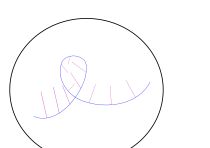
\includegraphics{/home/zack/SparkleShare/github.com/Notes/Class_Notes/2020/Spring/Moduli Spaces/sections/figures/2021-01-03_22-40}
};

\node (a) at (-7, 5) {\Huge ${\mathbb{P}}^3$};
\node[arrow_color] (a) at (1, -3) {\Huge Deformation};
\end{tikzpicture}
\end{center}

For \(i:C \hookrightarrow{\mathbb{P}}^3\), there is an exact sequence
\begin{align*}
0 \to I/I^2 \to &i^* \Omega_{{\mathbb{P}}^3} \to \Omega_\varepsilon\to 0 \\
&\Downarrow \quad \text{ taking duals } \\
0 \to T_C \to &i^* T_{{\mathbb{P}}^3} \to N_{C_{/{\mathbb{P}}^3} } \to 0
,\end{align*}
How do we compute \(T_{{\mathbb{P}}^3}\)? Fit into the exact sequence
\begin{align*}
0 \to {\mathcal{O}}\to i^* {\mathcal{O}}(1)^4 \to i^* T_{{\mathbb{P}}^3} \to 0
,\end{align*}
which we can restrict to \(C\).

We have
\(i^* {\mathcal{O}}(1) \cong {\mathcal{O}}_{{\mathbb{P}}^1}(3)\), so
\begin{align*}
0 \to H^0 {\mathcal{O}}_c \to &H^*({\mathcal{O}}(3)^4) \to H^0(i^* T_{{\mathbb{P}}^3}) \to 0 \\
&\Downarrow \\
0\to k \to &k^{16} \to k^{15} \to 0
.\end{align*}

This yields
\begin{align*}
0 \to H^0(T_c) \to &H^0(i^* T_{{\mathbb{P}}^3}) \to H^0(N_{C_{ /{\mathbb{P}}^3} }) \to H^1 T_c \\
&\Downarrow \\
0\to k^3 \to &k^{15} \to k^{12} \to 0
\end{align*}

\begin{example}[?]

\(\operatorname{Hilb}_{{\mathbb{P}}^n_k}^{P_?} \cong {\mathbb{P}}H^0({\mathbb{P}}^n, {\mathcal{O}}(d))^\vee\)
which has dimension \({n+1 \choose n} - 1\). Pick \(Z\) a \(k\) point in
this Hilbert scheme, then \(T_Z H = \hom(I_Z, {\mathcal{O}}_Z)\). Since
\(I_Z \cong {\mathcal{O}}_{{\mathbb{P}}}(-d)\) which fits into
\begin{align*}
0 \to {\mathcal{O}}_{{\mathbb{P}}^n}(-d) \to {\mathcal{O}}_{{\mathbb{P}}^n} \to {\mathcal{O}}_Z \to 0
.\end{align*}

We can identify
\begin{align*}
\hom(I_Z,{\mathcal{O}}_Z) = H^0( (I_Z/I_Z^2)^\vee) = H^0({\mathcal{O}}_Z(d))
.\end{align*}

\begin{center}
\begin{tikzcd}
0\ar[r] & {\mathcal{O}}_{{\mathbb{P}}^n}\ar[r]  & {\mathcal{O}}_{{\mathbb{P}}^n}(d)\ar[r]     & {\mathcal{O}}_Z(d)\ar[r]              & 0 \\
  &             &                   &                      &   \\
0\ar[r]  & H^0( {\mathcal{O}}_{{\mathbb{P}}^n}  ) \ar[r]  & H^0( {\mathcal{O}}_{{\mathbb{P}}^n}(d)  ) \ar[r]        & H^0({\mathcal{O}}_Z(d)  ) \ar[r]            & 0 \\
\text{dim:} & k           & k^{n+d \choose n} & k^{{n+d\choose n}-1} &
\end{tikzcd}
\end{center}

\end{example}

\begin{example}[?]

The tangent space of the following cubic:

\begin{center}
\begin{tikzpicture}
\node (node_one) at (0,0) {
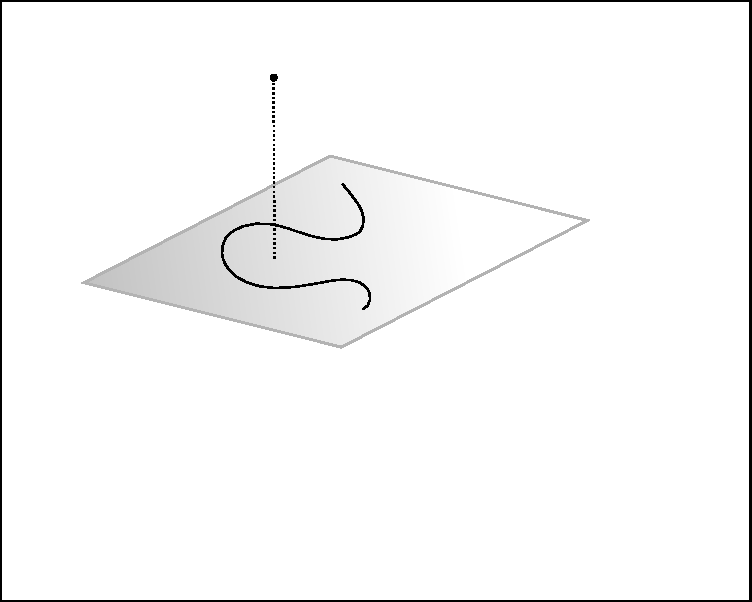
\includegraphics{/home/zack/SparkleShare/github.com/Notes/Class_Notes/2020/Spring/Moduli Spaces/sections/figures/2021-01-03_17-27}
};
\end{tikzpicture}
\end{center}

We can identify
\begin{align*}
\hom_{{\mathcal{O}}_k}(I_Z, {\mathcal{O}}_Z) = H^0((I_Z/I_Z^2)^\vee) = 3 + H^0((I_{Z_0}/I_{Z_0}^2)^\vee)
,\end{align*}

where the latter equals
\(H^0 \qty{ {\mathcal{O}}_1\mathrel{\Big|}_{z_0} \oplus {\mathcal{O}}(\zeta)\mathrel{\Big|}_{z_0} }\)
yielding
\begin{align*}
3+9 = 12
.\end{align*}

\end{example}

\hypertarget{uniform-vanishing-statements-thursday-january-30th}{%
\section{Uniform Vanishing Statements (Thursday January
30th)}\label{uniform-vanishing-statements-thursday-january-30th}}

Recall how we constructed the Hilbert scheme of hypersurfaces
\begin{align*}
\operatorname{Hilb}_{{\mathbb{P}}_k^n}^{P_{m, d}} = {\mathbb{P}}H^0({\mathbb{P}}^n; {\mathcal{O}}(d))^\vee
\end{align*}
A section \(\operatorname{Hilb}_{{\mathbb{P}}_k^n}^{P}(s)\) corresponds
to \(z\in {\mathbb{P}}^n_s\). We can look at the exact sequence

\begin{align*}
0 \to I_Z(m) \to {\mathcal{O}}_{{\mathbb{P}}_S^n} \xrightarrow{\text{restrict}} {\mathcal{O}}_z(m) \to 0
.\end{align*}

as \({\mathbb{P}}_s^n \xrightarrow{\pi_s} S\), so we can pushforward
along \(\pi\), which is left-exact, so

\begin{align*}
0 \to \pi_{s*} I_Z(m) \to \pi_{s*} {\mathcal{O}}_{{\mathbb{P}}_S^n}  = {\mathcal{O}}_S \otimes H^0({\mathbb{P}}^n; {\mathcal{O}}(m)) \to {\mathcal{O}}_z(m) \to R^1 \pi_{s*} I_Z(m) \to \cdots
.\end{align*}

\emph{Idea:} \(Z \subset {\mathbb{P}}_k^n\) will be determined (in
families!) by the space of degree \(d\) polynomials vanishing on \(Z\)
(?), i.e.
\begin{align*}
H^0({\mathbb{P}}^n, I_z(m)) \subset H^0({\mathbb{P}}^n, {\mathcal{O}}(m))
\end{align*}
for \(m\) very large. This would give a map of functors
\begin{align*}
\operatorname{Hilb}_{{\mathbb{P}}_k^n}^{P} \to {\operatorname{Gr}}(N, H^0({\mathbb{P}}^n, {\mathcal{O}}(m) ))
.\end{align*}
If this is a closed subfunctor, a closed subfunctor of a representable
functor is representable and we're done .

\begin{remark}

We need to get an \(m\) uniform in \(Z\), and more concretely:

\begin{enumerate}
\def\labelenumi{\arabic{enumi}.}
\item
  First need to make sense of what it means for \(Z\) to be determined
  by \(H^0({\mathbb{P}}^n, I_Z(m))\) for \(m\) only depending on \(P\).
\item
  This works point by point, but we need to do this in families. I.e.
  we'll use the previous exact sequence, and want the \(R^1\) to vanish.
\end{enumerate}

\end{remark}

\begin{slogan}

We need \emph{uniform} vanishing statements. There is a convenient way
to package the vanishing requirements needed here. From now on, take
\(k=\mkern 1.5mu\overline{\mkern-1.5muk\mkern-1.5mu}\mkern 1.5mu\) and
\({\mathbb{P}}^n = {\mathbb{P}}_k^n\).

\end{slogan}

\hypertarget{mhbox-regularity}{%
\subsection{\texorpdfstring{\(m{\hbox{-}}\)Regularity}{m\{\textbackslash hbox\{-\}\}Regularity}}\label{mhbox-regularity}}

\begin{definition}[m-Regularity of Coherent Sheaves]

A coherent sheaf \(F\) on \({\mathbb{P}}^n\) is
\textbf{\(m{\hbox{-}}\)regular} if \(H^i({\mathbb{P}}^n; F(m-i)) = 0\)
for all \(i> 0\).

\end{definition}

\begin{example}[?]

Consider \({\mathcal{O}}_{{\mathbb{P}}^n}\), this is
\(0{\hbox{-}}\)regular. Line bundles on \({\mathbb{P}}_n\) only have 0
and top cohomology. Just need to check that
\(H^n({\mathbb{P}}^n; {\mathcal{O}}(-n)) = 0\), but by Serre duality
this is
\begin{align*}
H^0({\mathbb{P}}^n; {\mathcal{O}}(n) \otimes\omega_{{\mathbb{P}}^n})^\vee= H^0({\mathbb{P}}^n; {\mathcal{O}}(-1))^\vee= 0
.\end{align*}

\end{example}

\begin{proposition}[?]

Assume \(F\) is \(m{\hbox{-}}\)regular. Then

\begin{enumerate}
\def\labelenumi{\arabic{enumi}.}
\item
  There is a natural multiplication map from linear forms on
  \({\mathbb{P}}^n\),
  \begin{align*}
    H^0({\mathbb{P}}^n; {\mathcal{O}}(1)) \otimes H^0({\mathbb{P}}^n; F(k)) \to H^0({\mathbb{P}}^n; F(k+1))
    ,\end{align*}
  which is surjective for \(k\geq n\).\footnote{Think of this as a
    graded module, this tells you the lowest number of small grade
    pieces needed to determine the entire thing.}
\item
  \(F\) is \(m'{\hbox{-}}\)regular for \(m' \geq m\).
\item
  \(F(k)\) is globally generated for \(k\geq m\), i.e.~the restriction
  \begin{align*}
    H^0({\mathbb{P}}^n; F(k)) \otimes{\mathcal{O}}_{{\mathbb{P}}^n} \to F(k) \to 0
    \end{align*}
  is exact (i.e.~surjective).
\end{enumerate}

\end{proposition}

\begin{example}[?]

\({\mathcal{O}}\) is \(m{\hbox{-}}\)regular for \(m \geq 0\) implies
\({\mathcal{O}}(k)\) is \(-k{\hbox{-}}\)regular and is also
\(m{\hbox{-}}\)regular for\(m\geq -k\).

\end{example}

\hypertarget{proof-of-2-and-3}{%
\subsubsection{Proof of 2 and 3}\label{proof-of-2-and-3}}

Induction on dimension of \(n\) in \({\mathbb{P}}^n\). Coherent sheaves
on \({\mathbb{P}}^0\) are vector spaces, so no higher cohomology.

\begin{proof}[Step 1]

Take a generic hyperplane \(H \subset {\mathbb{P}}^n\), there is an
exact sequence
\begin{align*}
0 \to {\mathcal{O}}(-1) \to {\mathcal{O}}\to {\mathcal{O}}_H \to 0
.\end{align*}

where \({\mathcal{O}}_H\) is the structure sheaf. Tensoring with \(H\)
remains exact, so we get
\begin{align*}
0 \to F(-1) \to F \to F_H \to 0
.\end{align*}

Why? \({\mathbb{A}}^n \subset {\mathbb{P}}^n\), let
\(A = {\mathcal{O}}_{{\mathbb{P}}^n}({\mathbb{A}}^n)\) be the polynomial
ring over \({\mathbb{A}}^n\). Then the restriction of the first sequence
to \({\mathbb{A}}^n\) yields
\begin{align*}
0 \to A \xrightarrow{f} A \to A/f \to 0
,\end{align*}
and thus we want
\begin{align*}
F \xrightarrow{f} F \to F/fF \to 0
\end{align*}
which results after restricting the second sequence to
\({\mathbb{A}}^n\). Thus we just want \(f\) to not be a zero divisor. If
we take \(f\) not vanishing on any associated point of \(F\), then this
will be exact. Associated points: generic points arising by supports of
sections of \(F\). \(F\) is coherent, so it has finitely many associated
points. If \(H\) does not contain any of the associated points of \(F\),
then the second sequence is indeed exact.

\end{proof}

\begin{proof}[Step 2]

Twist up by \(k\) to obtain
\begin{align*}
0 \to F(k-1) \to F(k) \to F_H(k) \to 0
.\end{align*}
Look at the LES in cohomology to get
\begin{align*}
H^i(F(m-i)) \to H^i(F_H(m-i)) \to H^{i+1}(F(m - (i+1)))
.\end{align*}
So \(F_H\) is \(m{\hbox{-}}\)regular. By induction, this proves
statements 1 and 2 for all \(F_H\). So take \(k = m+1-i\) and consider
\begin{align*}
H^i(F(m-i)) \to H^i(F(m+1-i)) \to H^i(F_H(m+1-i))
.\end{align*}
We know 2 is satisfied, so the RHS is zero, and we know the LHS is zero,
so the middle term is zero. Thus \(F\) itself is \(m+1\) regular, and by
inducting on \(m\) we get statement 2.

\end{proof}

By multiplication maps, we get a commutative diagram:

\begin{center}
\begin{tikzcd}
                                                        &  & H^0({\mathcal{O}}(1)) \otimes H^0(F(k)) \arrow[dd, "\beta"] \arrow[rrr] \arrow[rrrdd] &  &  & H^0({\mathcal{O}}(1))\otimes H^0(F_H(k)) \arrow[dd] \\
                                                        &  &                                                                             &  &  &                                           \\
H^0(F(k)) \arrow[rr, "H"] \arrow[rruu, "H \otimes\operatorname{id}"] &  & H^0(F(k+1)) \arrow[rrr, "\alpha", dashed]                                   &  &  & H^0(F_H(k+1))
\end{tikzcd}
\end{center}

We'd like to show the diagonal map is surjective.

\begin{observation}

\envlist

\begin{enumerate}
\def\labelenumi{\arabic{enumi}.}
\item
  The top map is a surjection, since
  \begin{align*}
  H^0(F(k)) \to H^0(F_H(k)) \to H^1(F(k-1)) = 0
  \end{align*}
  for \(k\geq m\) by (2).
\item
  The right-hand map is surjective for \(k\geq m\).
\item
  \(\ker(\alpha) \subset \operatorname{im}(\beta)\) by a small diagram
  chase, so \(\beta\) is surjective.
\end{enumerate}

This shows (1) and (2) completely.

\end{observation}

\begin{proof}[of 3]

We know \(F(k)\) is globally generated for \(k\gg 0\). Thus for all
\(k\geq m\), \(F(k)\) is globally generated by (1).

\end{proof}

\begin{theorem}[?]

Let \(P \in {\mathbb{Q}}[t]\) be a Hilbert polynomial. There exists an
\(m_0\) only depending on \(P\) such that for all subschemes
\(Z \subset {\mathbb{P}}^n_k\) with Hilbert polynomial \(P_Z = P\), the
ideal sheaf \(I_z\) is \(m_0{\hbox{-}}\)regular.

\end{theorem}

\hypertarget{proof-of-theorem}{%
\subsubsection{Proof of Theorem}\label{proof-of-theorem}}

Induct on \(n\). For \(n=0\), again clear because higher cohomology
vanishes and there are no nontrivial subschemes. For a fixed \(Z\), pick
\(H\) in \({\mathbb{P}}^n\) (and setting \(I \coloneqq I_z\) for
notation) such that
\begin{align*}
0 \to I(-1) \to I \to I_H \to 0
.\end{align*}
is exact. Note that the Hilbert polynomial
\(P_{I_H}(t) = P_I(t) - P_I(t-1)\) and
\(P_I = P_{{\mathcal{O}}_{{\mathbb{P}}^n}} - P_Z\). By induction, there
exists some \(m_1\) depending only on \(P\) such that \(I_H\) is
\(m_1{\hbox{-}}\)regular. We get
\begin{align*}
H^{i-1}(I_H(k)) \to H^i(I(k-1)) \to H^i(I(k)) \to H^i(I_H(k))
,\end{align*}
and for \(k\geq m_1 - i\) the LHS and RHS vanish so we get an
isomorphism in the middle. By Serre vanishing, for \(k \gg 0\) we have
\(H^i(I(k)) = 0\) and thus \(H^i(I(k)) = 0\) for \(k\geq m_i - i\). This
works for all \(i > 1\), we have \(H^i(I(m_i - i)) = 0\). We now need to
find \(m_0 \geq m_1\) such that \(H^1(I(m_0 - 1)) = 0\) (trickiest part
of the proof).

\begin{lemma}[?]

The sequence \(\qty{\dim H^1(I(k))}_{k\geq m_i - 1}\) is \emph{strictly}
decreasing.\footnote{Note: \(h^1 = \dim H^1\).}

\end{lemma}

\begin{remark}

Given the lemma, it's enough to take \(m_0 \geq m_1 + h^1(I(m_1 - 1))\).
Consider the LES we have a surjection
\begin{align*}
H^0({\mathcal{O}}_Z(m_1 - 1)) \to H^1(I(m_1 - 1)) \to 0
.\end{align*}
So the dimension of the LHS is equal to \(P_Z(m_1 - 1)\), using the fact
that terms vanish and make the Euler characteristic equal to \(P_Z\).
Thus we can take \(m_0 = m_1 + P(m_1 - 1)\).

\end{remark}

\begin{proof}[of Lemma]

Considering the LES
\begin{align*}
H^0(I(k+1)) \xrightarrow{\alpha_{k+1}} H^0(I_H(k+1)) \to H^1(I(k)) \to H^1(I(k+1)) \to 0
,\end{align*}
where the last term is zero because \(I_H\) is \(m_1{\hbox{-}}\)regular.
So the sequence \(h^1(I(k))\) is non-increasing.

\begin{observation}

If it does \emph{not} strictly decrease for some \(k\), then there is an
equality on the RHS, which makes \(\alpha_{k+1}\) surjective. This means
that \(\alpha_{k+2}\) is surjective, since
\begin{align*}
H^0({\mathcal{O}}(1)) \otimes H^0(I_H(k+1)) \twoheadrightarrow H^0(I_H(k+2))
.\end{align*}

\end{observation}

So if one is surjective, everything above it is surjective, but by Serre
vanishing we eventually get zeros. So \(\alpha_{k+i}\) is surjective for
all \(i\geq 1\), contradicting Serre vanishing, since the RHS are
isomorphisms for all \(k\).

\end{proof}

Thus for any \(Z\subset {\mathbb{P}}^n_k\) with \(P_Z = P\), we
uniformly know that \(I_Z\) is \(m_0{\hbox{-}}\)regular for some \(m_0\)
depending only on \(P\).

\begin{claim}

\(Z\) is determined by the degree \(m_0\) polynomials vanishing on
\(Z\), i.e.~\(H^0(I_z(m_0))\) as a subspace of all degree \(m_0\)
polynomials \(H^0({\mathcal{O}}(m_0))\) and has fixed dimension. We have
\(H^i(I_Z(m_0)) = 0\) for all \(i> 0\), and in particular
\(h^0(I_Z(m_0)) = P(m_0)\) is constant.

\end{claim}

It is determined by these polynomials because we have a sequence
\begin{align*}
0 \to I_Z(m_0) \to {\mathcal{O}}(m_0) \to {\mathcal{O}}_Z(m_0) \to 0
.\end{align*}

We can get a commuting diagram over it
\begin{align*}
0 \to H^0(I_Z(m_0)) \otimes{\mathcal{O}}_{{\mathbb{P}}^n} \to H^0({\mathcal{O}}(m_0)) \otimes{\mathcal{O}}_{{\mathbb{P}}^n} \to \cdots
\end{align*}
where the middle map down is just evaluation and.the first map down is a
surjection. Hence \(I_Z(m_0)\), hence \({\mathcal{O}}_Z\), hence \(Z\)
is determined by \(H^0(I_Z(m_0))\).

\begin{quote}
Next time: we'll show that this is a subfunctor that is locally closed.
\end{quote}

\hypertarget{thursday-february-6th}{%
\section{Thursday February 6th}\label{thursday-february-6th}}

\begin{quote}
Review base-change!
\end{quote}

For \(k=\mkern 1.5mu\overline{\mkern-1.5muk\mkern-1.5mu}\mkern 1.5mu\),
and \(C_{/k}\) a smooth projective curve, then
\(\operatorname{Hilb}_{C_{/k}}^n = \operatorname{Sym}^n C\).

\begin{definition}[The Hilbert-Chow Map]

For \(X_{_{/k}}\) a smooth projective \emph{surface},
\(\operatorname{Hilb}_{X_{_{/k}}}^n \neq \operatorname{Sym}^n X\), there
is a map (the Hilbert-Chow map)
\begin{align*}
\operatorname{Hilb}_{X_{_{/k}}}^n &\to \operatorname{Sym}^n X \\
Z &\mapsto {\operatorname{supp}}(Z) \\
U  = \text{reduced subschemes} &\mapsto U' = \text{ reduced multisets } \\
{\mathbb{P}}^1 &\mapsto (x, x)
.\end{align*}

\end{definition}

\begin{example}[?]

Consider \({\mathbb{A}}^2 \times{\mathbb{A}}^2\) under the
\({\mathbb{Z}}/2{\mathbb{Z}}\) action
\begin{align*}
( (x_1, y_1), (x_2, y_2)) \mapsto ((x_2, y_2), (x_1, y_1))
.\end{align*}

Then
\begin{align*}
({\mathbb{A}}^2)^2 / {\mathbb{Z}}/2{\mathbb{Z}}
&= \operatorname{Spec}k[x_1, y_1, x_2, y_2]^{{\mathbb{Z}}/2{\mathbb{Z}}} \\
&= \operatorname{Spec}k[x_1 x_2, y_1 y_2, x_1 + x_2, y_1 + y_2, x_1 y_2 + x_2 y_1, \cdots]
\end{align*}
with a bunch of symmetric polynomials adjoined.

\end{example}

\begin{example}[?]

Take \({\mathbb{A}}^2\) and consider
\(\operatorname{Hilb}_{{\mathbb{P}}^2}^3\). If \(I\) is a monomial ideal
in \({\mathbb{A}}^2\), there is a nice picture. We can identify the
tangent space
\begin{align*}
T_Z \operatorname{Hilb}_{{\mathbb{P}}^2}^n = \hom_{{\mathcal{O}}_{{\mathbb{P}}^2}} ( I_2, {\mathcal{O}}_Z) = \bigoplus \hom(I_{Z_i}, {\mathcal{O}}_{Z_i})
.\end{align*}
if \(Z = {\coprod}Z_i\). If \(I\) is supported at 0, then we can
identify the ideal with the generators it leaves out.

\end{example}

\begin{example}[?]

\(I = (x^2, xy, y^2)\):

\begin{figure}
\centering
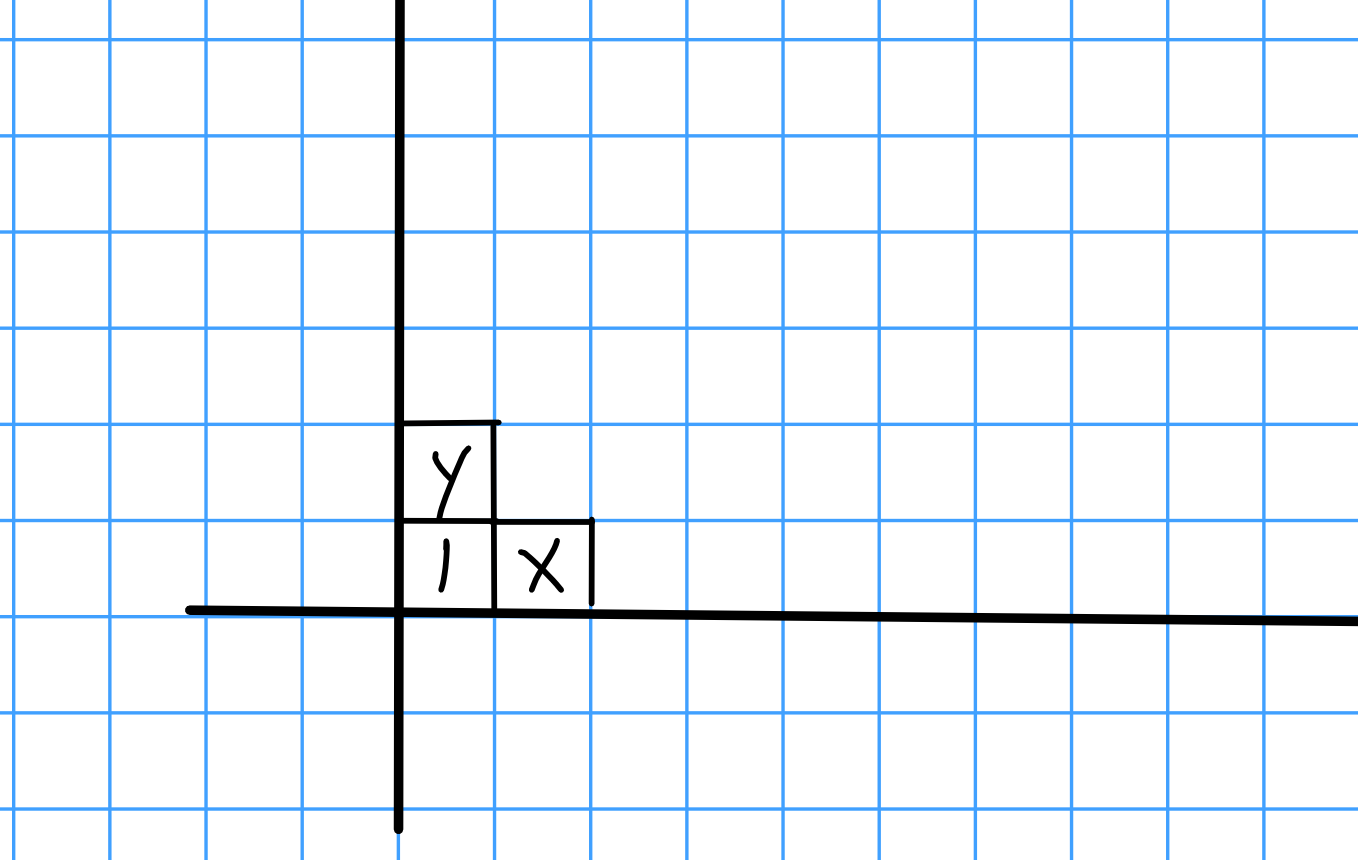
\includegraphics[width=3.64583in,height=\textheight]{figures/2020-02-06-12:48.png}
\caption{Image}
\end{figure}

\end{example}

\begin{example}[?]

\(I = (x^6, x^2y^2, xy^4, y^5)\):

\begin{figure}
\centering
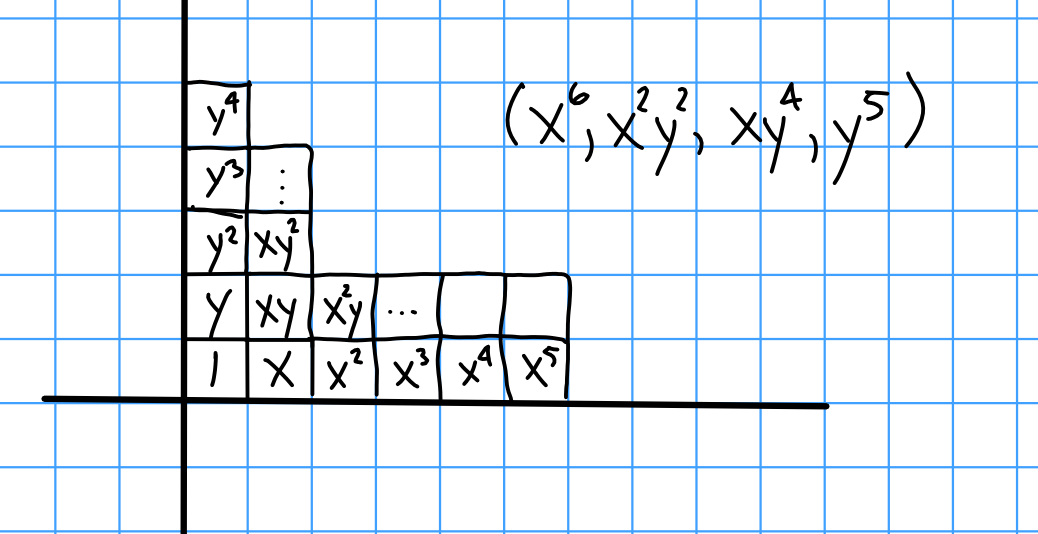
\includegraphics[width=3.64583in,height=\textheight]{figures/2020-02-06-12:49.png}
\caption{Image}
\end{figure}

\end{example}

\begin{example}[?]

\(I = (x^2, y)\). Let \(e=x^2, f = y\).

\begin{figure}
\centering
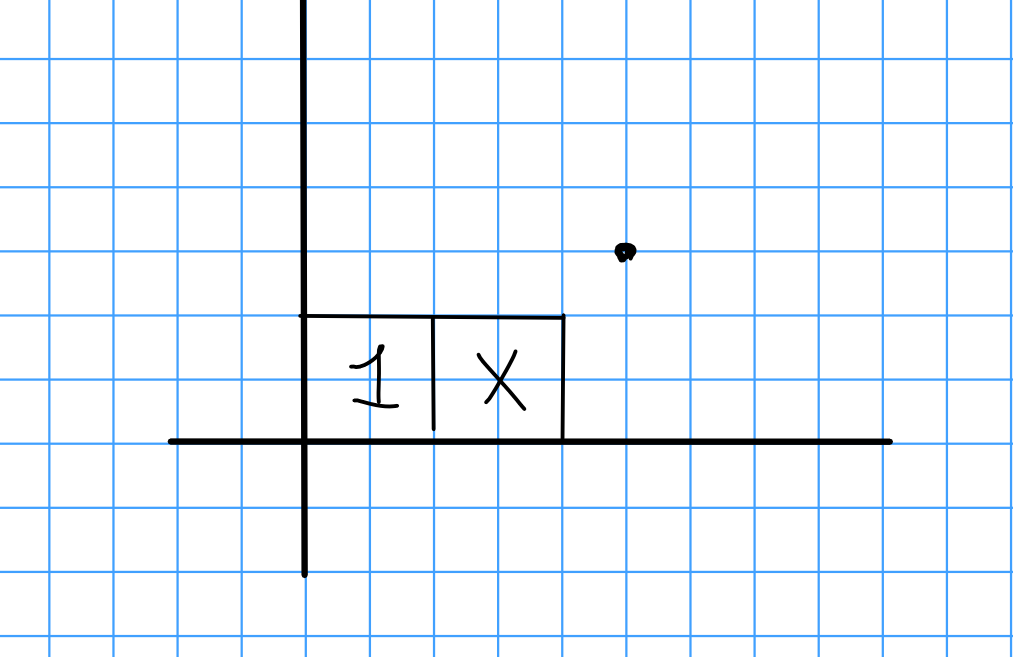
\includegraphics[width=3.64583in,height=\textheight]{figures/2020-02-06-12:54.png}
\caption{Image}
\end{figure}

By comparing rows to columns, we obtain a relation \(ye = x^2 f\). Write
\({\mathcal{O}}= \left\{{1, x}\right\}\), then note that this relation
is trivial in \({\mathcal{O}}\) since \(y=x^2=0\). Thus
\(\hom(I, {\mathcal{O}}) = \hom(k^2, k^2)\) is 4-dimensional.

\end{example}

\begin{remark}

Note that \(C_{_{/k}}\) for curves is an important case to know. Take
\(Z \subset C \times C^n\), then quotient by the symmetric group \(S^n\)
(need to show this can be done), then
\(Z/S^n \subset C \times\operatorname{Sym}^n C\) and composing with the
functor \(\operatorname{Hilb}\) represents yields a map
\(\operatorname{Sym}^n C \to \operatorname{Hilb}_{C_{/k}}^n\). This is
bijective on points, and a tangent space computation shows it's an
isomorphism.

\end{remark}

\begin{example}[?]

Consider the nodal cubic in \({\mathbb{P}}^2\):

\begin{figure}
\centering
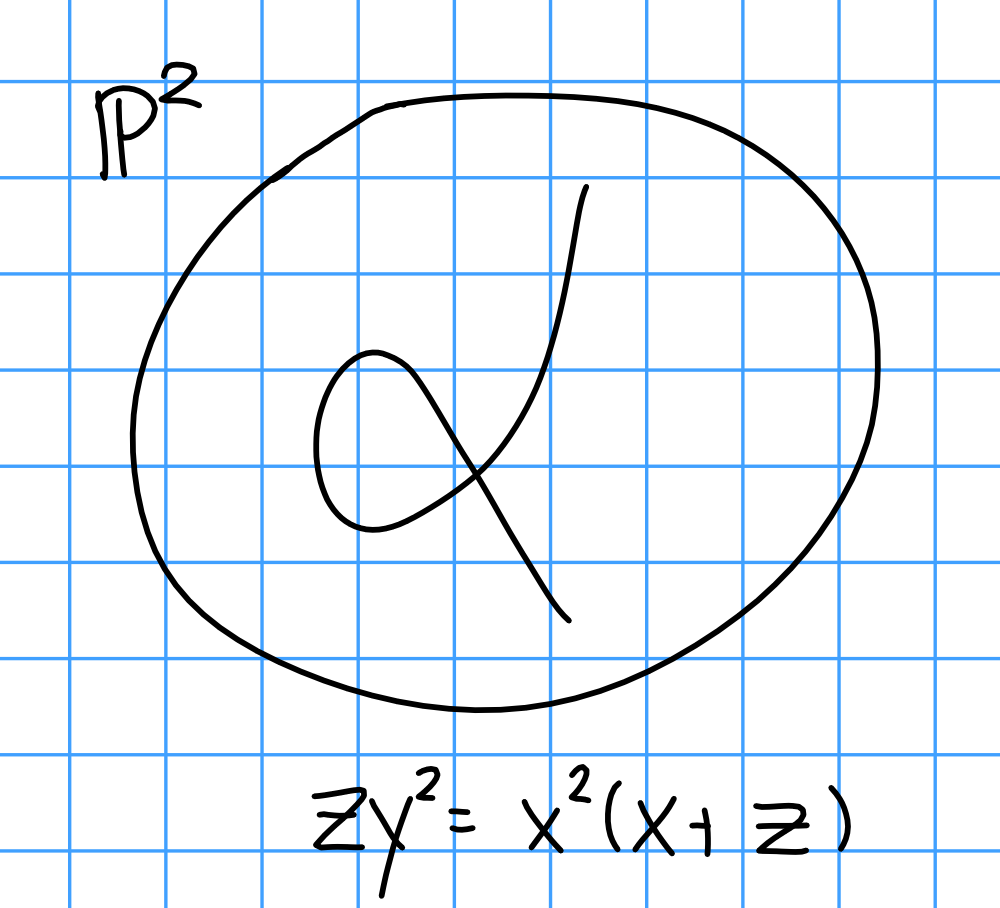
\includegraphics[width=3.64583in,height=\textheight]{figures/2020-02-06-13:01.png}
\caption{Nodal cubic}
\end{figure}

\begin{quote}
The nodal cubic \(zy^2 = x^2(x+z)\).
\end{quote}

Consider the open subscheme \(V \subset \operatorname{Hilb}_{C_{/k}}^2\)
of points \(z \subset U\) for \(U \subset C\) open. We can normalize:

\begin{figure}
\centering
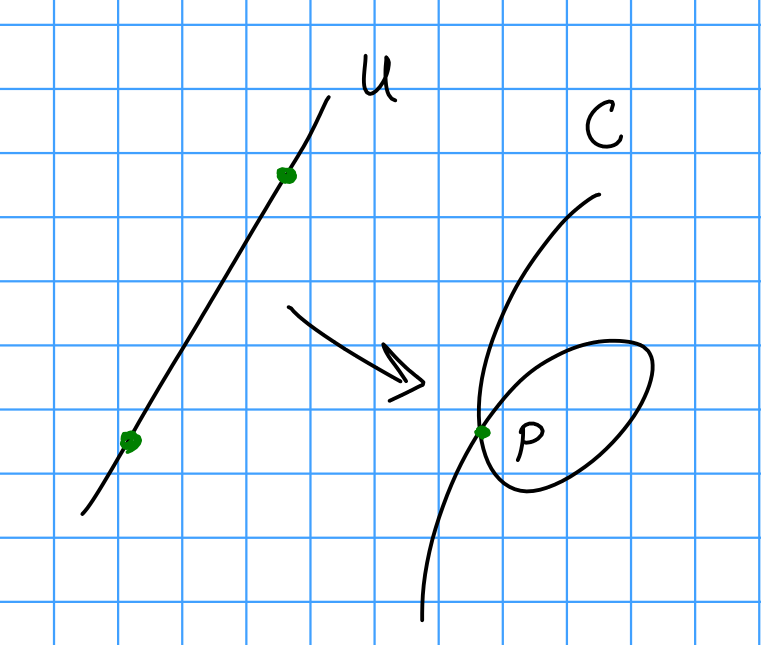
\includegraphics[width=3.64583in,height=\textheight]{figures/2020-02-06-13:03.png}
\caption{Normalized cubic}
\end{figure}

This yields a map fro \({\mathbb{P}}^1 \setminus\text{2 points}\). This
gives us a stratification, i.e.~a locally closed embedding
\begin{align*}
(\text{z supported on U}) {\coprod}(\text{1 point at p}) {\coprod}(\text{both points at p}) \to \operatorname{Hilb}_{C_{/k}}^2
.\end{align*}

The first locus is given by the complement of two lines:

\begin{figure}
\centering
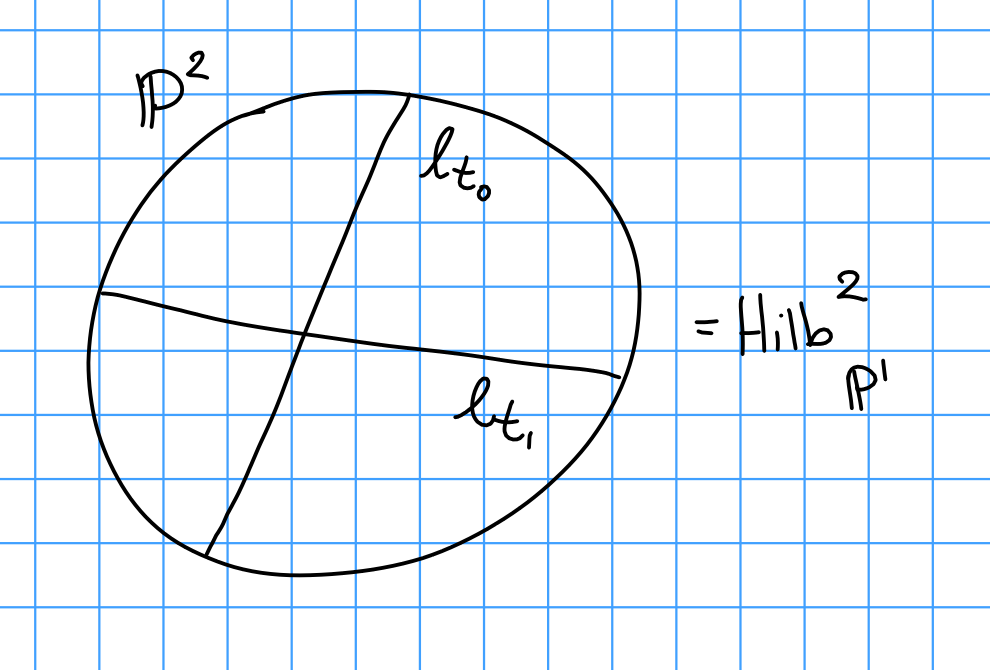
\includegraphics[width=3.64583in,height=\textheight]{figures/2020-02-06-13:08.png}
\caption{Locus 1}
\end{figure}

The third locus is given by arrows at \(p\) pointing in any direction,
which gives a copy of \({\mathbb{P}}^1\). The second is
\({\mathbb{P}}^1\) minus two points. Above each point is a nodal cubic
with two marked points, and moving the base point towards a line
correspond to moving one of the points toward the node:

\begin{figure}
\centering
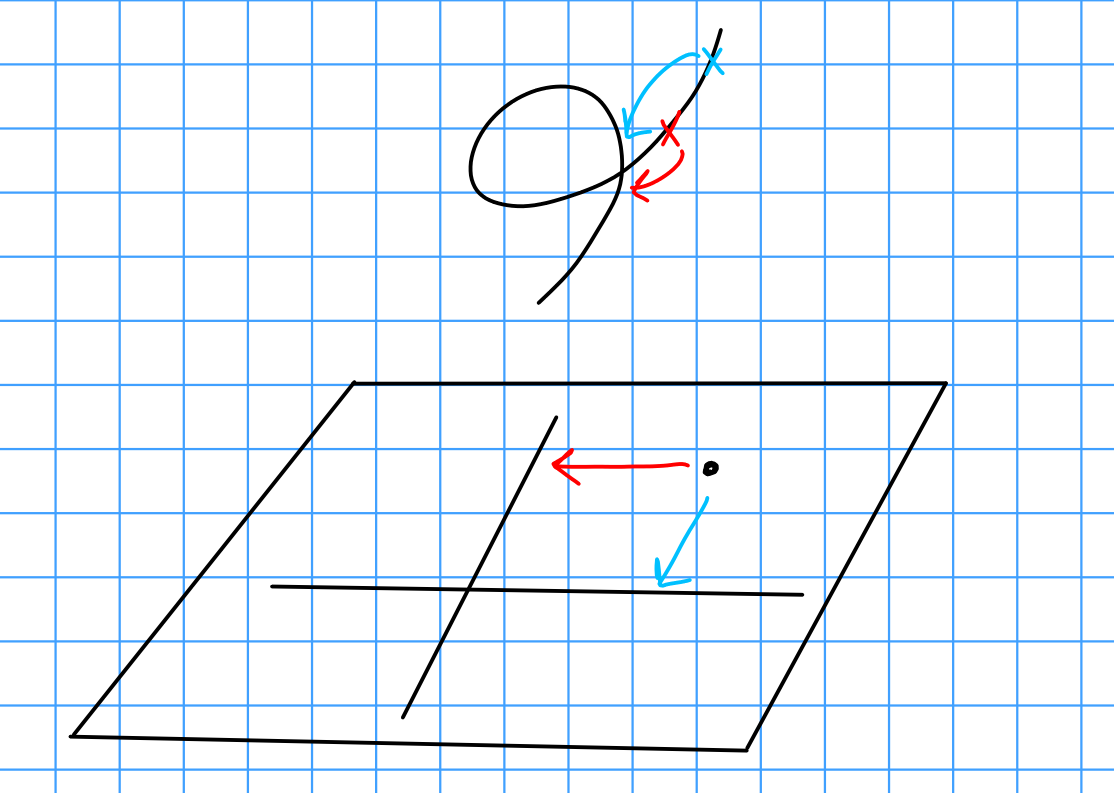
\includegraphics[width=3.64583in,height=\textheight]{figures/2020-02-06-13:11.png}
\caption{Moving base toward the point}
\end{figure}

More precisely, we're considering the cover
\({\mathbb{P}}^1 \setminus\text{2 points} \to C\) and thinking about
ways in which two points and approach the missing points. These give
specific tangent directions at the node on the cubic, depending on how
this approach happens -- either both points approach missing point \#1,
both approach missing point \#2, or each approach a separate missing
point.

\end{example}

\begin{remark}

Useful example to think about. Not normal, reduced, but glued in a weird
way. Possibly easier to think about: cuspidal cubic.

\end{remark}

\hypertarget{representability-1}{%
\subsection{Representability}\label{representability-1}}

Recall the following definition:

\begin{definition}[$m\dash$Regularity]

A coherent sheaf \(F\) on \({\mathbb{P}}_k^n\) for \(k\) a field is
\(m{\hbox{-}}\)regular iff \(H^i(F(m-i)) = 0\) for all \(i> 0\).

\end{definition}

\begin{proposition}[?]

For every Hilbert polynomial \(P\), there exists some \(m_0\) depending
on \(P\) such that any \(Z \subset {\mathbb{P}}^n_k\) with \(P_Z = P\)
satisfies \(I_Z\) is \(m{\hbox{-}}\)regular.

\end{proposition}

\begin{remark}[1]

\(F\) is \(m{\hbox{-}}\) regular iff
\(\mkern 1.5mu\overline{\mkern-1.5muF\mkern-1.5mu}\mkern 1.5mu = F \times_{\operatorname{Spec}k} \operatorname{Spec}\mkern 1.5mu\overline{\mkern-1.5muk\mkern-1.5mu}\mkern 1.5mu\)
is \(m{\hbox{-}}\)regular.

\end{remark}

\begin{remark}[2]

The \(m_0\) produced does not depend on \(k\).

\end{remark}

\begin{lemma}[?]

For \(m_0 = m_0(P)\) and \(N = N(P)\), we have an embedding as a
subfunctor
\begin{align*}
\operatorname{Hilb}_{{\mathbb{P}}^m_{\mathbb{Z}}}^P \to {\operatorname{Gr}}(N, H^0( {\mathbb{P}}^n_{\mathbb{Z}}, {\mathcal{O}}(m_0)  )^\vee)
.\end{align*}

\end{lemma}

For any \(Z \subset {\mathbb{P}}^n_S\) flat over \(S\) with
\(P_{Z_s} = P\) for all \(s\in S\) points, we want to send this to
\begin{align*}
0\to R^\vee\to {\mathcal{O}}_s \otimes H^0({\mathbb{P}}^n_{\mathbb{Z}}, {\mathcal{O}}(m_0))^\vee\to Q \to 0
\end{align*}
or equivalently
\begin{align*}
0 \to Q^\vee\to {\mathcal{O}}_s \otimes H^0({\mathbb{P}}^n_{\mathbb{Z}}, {\mathcal{O}}(m_0)) \to R \to 0
\end{align*}
with \(R\) locally free.

So instead of the quotient \(Q\) being locally free, we can ask for the
sub \(Q^\vee\) to be locally free instead, which is a weaker condition.

We thus send \(Z\) to
\begin{align*}
0 \to \pi_{s*} I_Z(m_0) \to \pi_{s*} {\mathcal{O}}_{{\mathbb{P}}^n_s}(m_0) = {\mathcal{O}}_s \otimes H^0({\mathbb{P}}^n, {\mathcal{O}}(m_0))
\end{align*}
which we obtain by taking the pushforward from this square:

\begin{center}
\begin{tikzcd}
{\mathbb{P}}^n_s \arrow[dd, "\pi_s"] \arrow[rr] &  & {\mathbb{P}}^n_Z \arrow[dd] \\
                                &  &                    \\
S \arrow[rr]                           &  & \operatorname{Spec}{\mathbb{Z}}
\end{tikzcd}
\end{center}

We have a sequence
\(0 \to I_Z(m_0) \to {\mathcal{O}}(m_0) \to {\mathcal{O}}_Z(m_0) \to 0\).
Thus we get a sequence

\begin{align*}
0 \to \pi_{s*}I_Z(m_0) \to \pi_{s*}{\mathcal{O}}(m_o) \to \pi_{s*} {\mathcal{O}}_Z(m_0) \to R^1 \pi_{s*}I_Z(m_0) \to \cdots
.\end{align*}

\hypertarget{step-1}{%
\subsubsection{Step 1}\label{step-1}}

\begin{align*}
R^1\pi_* I_Z(m_0) = 0
.\end{align*}

By base change, it's enough to show that \(H^1(Z_s, I_{Z_s}(m_0)) = 0\).
This follows by \(m_0{\hbox{-}}\)regularity.

\hypertarget{step-2}{%
\subsubsection{Step 2}\label{step-2}}

\(\pi_{s*}I_Z(m_0)\) and \(\pi_{s*} {\mathcal{O}}_Z(m_0)\) are locally
free. For all \(i>0\), we have

\begin{itemize}
\tightlist
\item
  \(R^i \pi_{s*} I_Z(m_0) = 0\) by \(m_0{\hbox{-}}\)regularity,
\item
  \(R^i \pi_{s*} {\mathcal{O}}(m_0) = 0\) by base change,
\item
  and thus \(R^i \pi_{s*} {\mathcal{O}}_Z(m_0) = 0\).
\end{itemize}

\hypertarget{step-3}{%
\subsubsection{Step 3}\label{step-3}}

\(\pi_{s*}I_Z(m_0)\) has rank \(N = N(P)\).

Again by base change, there is a map
\(\pi_* I_Z(m_0) \otimes k(s) \to H^0(Z_S, I_{Z_s}(m_0))\) which we know
is an isomorphism. Because \(h^i ( I_{Z_S}(m_0) ) = 0\) for \(i>0\) by
\(m{\hbox{-}}\)regularity and
\begin{align*}
h^0(I_{Z_S}(m_0)) = P_{\mathcal{O}}(m_0) - P_{{\mathcal{O}}_{Z_s}}(m_0) = P_{\mathcal{O}}(m_0) - P(m_0)
.\end{align*}

This yields a well-defined functor
\begin{align*}
\operatorname{Hilb}_{{\mathbb{P}}^n_{\mathbb{Z}}}^P \to {\operatorname{Gr}}(N, H^0({\mathbb{P}}^n, {\mathcal{O}}(m_0))^\vee)
.\end{align*}

\begin{remark}

Note that we've just said what happens to objects; strictly speaking we
should define what happens for morphisms, but they're always give by
pullback.

\end{remark}

We want to show injectivity, i.e.~that we can recover \(Z\) from the
data of a number f polynomials vanishing on it, which is the data
\(0 \to \pi_{s*} I_Z(m_0) \to {\mathcal{O}}_s \otimes H^0({\mathbb{P}}^n, {\mathcal{O}}(m_0))\).

Given
\begin{align*}
0 \to Q^\vee\to {\mathcal{O}}_s \otimes H^0({\mathbb{P}}^n, {\mathcal{O}}(m_0)) = \pi_{s*} {\mathcal{O}}_{{\mathbb{P}}^n_S}(m_0)
\end{align*}
we get a diagram

\begin{center}
\begin{tikzcd}
\pi_{s}^* Q^\vee\arrow[rrdd] \arrow[rrr] &  &                          & {\mathcal{O}}_{{\mathbb{P}}^n_s}(m_0) \\
                                  &  &                          &                    \\
                                  &  & I(m_0) \arrow[ruu, hook] &
\end{tikzcd}
\end{center}

where \(Q^\vee= \pi_{s*} I_Z(m_0)\), so we're looking at

\begin{center}
\begin{tikzcd}
Q^\vee= \pi_{s*}^* \pi_{s*} I_Z(m_0) 
  \arrow[rrdd, twoheadrightarrow] 
  \arrow[rrr] 
&  
&                          
& {\mathcal{O}}_{{\mathbb{P}}^n_s}(m_0) 
\\
&  
&                          
&                    
\\
&  
& I(m_0) 
  \arrow[ruu, hook] 
&
\end{tikzcd}
\end{center}

The surjectivity here follows from
\({\mathcal{O}}_{Z_s} \otimes H^0(I_{Z_s}(m_0)) \to I_{Z_s}(m_0)\) (?).
Given a universal family
\(G = {\operatorname{Gr}}( N, H^0({\mathcal{O}}(m_0))^\vee)\) and
\(Q^\vee\subset {\mathcal{O}}_G \otimes H^0({\mathcal{O}}(m_0))^\vee\),
we obtain \(I_W \subset {\mathcal{O}}_G\) and
\(W \subset {\mathbb{P}}^n_G\).

\hypertarget{tuesday-february-18th}{%
\section{Tuesday February 18th}\label{tuesday-february-18th}}

\begin{theorem}[?]

Let \(X/S\) be a projective subscheme (i.e.~\(X\subset {\mathbb{P}}^n\)
for some \(n\)). The Hilbert functor of flat families
\(\operatorname{Hilb}_{X/S}^p\) is representable by a projective
\(S{\hbox{-}}\)scheme.

\end{theorem}

\begin{remark}

Note that without a fixed \(P\), this is \emph{locally} of finite type
but not finite type. After fixing \(P\), it becomes finite type.

\end{remark}

\begin{example}[?]

For a curve of genus \(g\), there is a smooth family
\({\mathcal{C}}\xrightarrow{\pi} S\) with \(S\) finite-type over
\({\mathbb{Z}}\) where every genus \(g\) curve appears as a fiber. I.e.,
genus \(g\) curves form a \emph{bounded family} (here there are only
finitely many algebraic parameters to specify a curve). How did we
construct? Take the third power of the canonical bundle and show it's
very ample, so it embeds into some projective space and has a Hilbert
polynomial.

\end{example}

In fact, there is a finite type \emph{moduli stack}
\({\mathcal{M}}_g / {\mathbb{Z}}\) of genus \(g\) curves. There will be
a map \(S \twoheadrightarrow{\mathcal{M}}_g\), noting that
\({\mathcal{C}}\) is not a moduli space since it may have redundancy.
We'll use the fact that a finite-type scheme surjects onto
\({\mathcal{M}}_g\) to show it is finite type.

\begin{remark}

If \(X/S\) is proper, we can't talk about the Hilbert polynomial, but
the functor \(\operatorname{Hilb}_{X/S}\) is still representable by a
locally finite-type scheme with connected components which are proper
over \(S\).

\end{remark}

\begin{remark}

If \(X/S\) is \emph{quasiprojective} (so locally closed,
i.e.~\(X\hookrightarrow{\mathbb{P}}^n_S\)), then
\(\operatorname{Hilb}_{X/S}^P(T) \coloneqq\left\{{z\in X_T \text{ projective, flat over S with fiberwise Hilbert polynomial P }}\right\}\)
is still representable, but now by a quasiprojective scheme.

\end{remark}

\begin{example}[?]

Length \(Z\) subschemes of \({\mathbb{A}}^1\): representable by
\({\mathbb{A}}^2\).

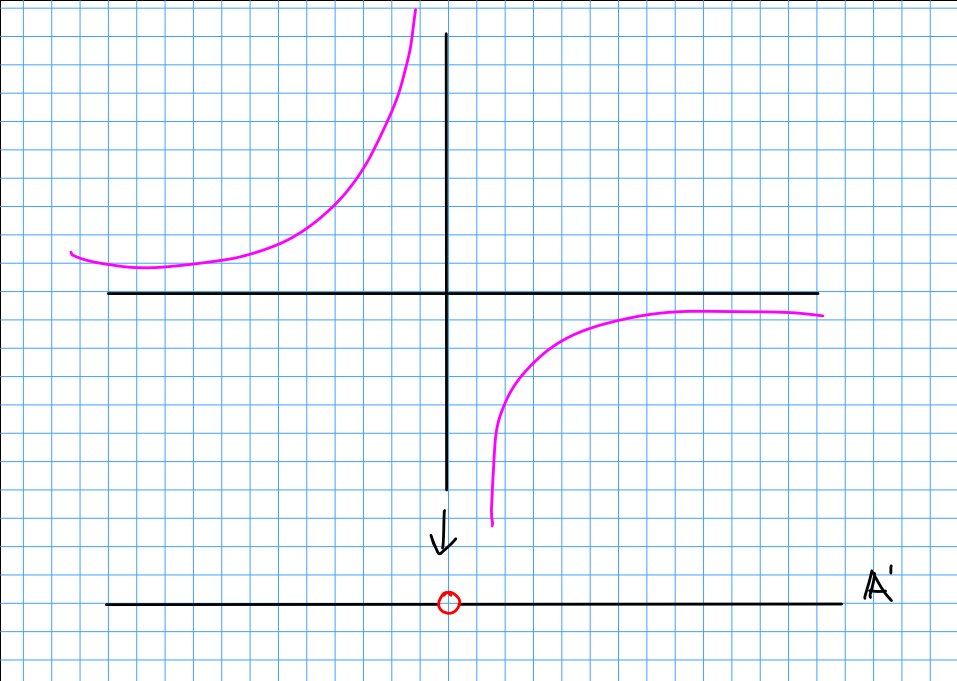
\includegraphics{figures/2020-02-18-12:46.png}\\

Upstairs: parametrizing length 1 subschemes, i.e.~points.

\end{example}

\begin{remark}

If \(X\subset {\mathbb{P}}_S^n\) and \(E\) is a coherent sheaf on \(X\),
then
\begin{align*}
\operatorname{Quot}_{E, X/S}^{P}(T) = \left\{{ j^*E \to F \to 0, \text{ over } X_T \to T,~F \text{ flat with fiberwise Hilbert polynomial  } P  }\right\}
\end{align*}
where \(T \xrightarrow{g} S\) is representable by an
\(S{\hbox{-}}\)projective scheme.

\end{remark}

\begin{example}[?]

Take \(E = {\mathcal{O}}_x\), \(X\) and \(S\) a point, and \(E\) is a
vector space, then
\(\operatorname{Quot}_{E/S}^P = {\operatorname{Gr}}(\operatorname{rank}, E)\).

\end{example}

\begin{warnings}

The Hilbert scheme of 2 points on a surface is more complicated than
just the symmetric product.

\end{warnings}

\begin{example}[?]

\begin{align*}
\qty{{\mathbb{A}}^2}^3 &\to \qty{{\mathbb{A}}^2}^2 \\
\supseteq \Delta\coloneqq\Delta_{01} \times\Delta_{02} &\to \qty{{\mathbb{A}}^2}^2
\end{align*}

where \(\Delta_{ij}\) denote the diagonals on the \(i, j\) factors. Here
all associate points of \(\Delta\) dominate the image, but it is not
flat. Note that if we take the complement of the diagonal in the image,
then the restriction \(\Delta' \to \qty{{\mathbb{A}}^2}^2\setminus D\)
is in fact flat.

\end{example}

\begin{example}[Mumford]

The Hilbert scheme may have nontrivial scheme structure, i.e.~this will
be a ``nice'' Hilbert scheme with is generally not reduced. We will find
a component \(H\) of a \(\operatorname{Hilb}_{{\mathbb{P}}^3_C}^P\)
whose generic point corresponds to a smooth irreducible
\(C\subset {\mathbb{P}}^3\) which is generically non-reduced.

\end{example}

\hypertarget{cubic-surfaces}{%
\subsection{Cubic Surfaces}\label{cubic-surfaces}}

\begin{quote}
See Hartshorne Chapter 5.
\end{quote}

Let \(X\subset {\mathbb{P}}^3\) be a smooth cubic surface, then
\({\mathcal{O}}(1)\) on \({\mathbb{P}}^3\) restricts to a divisor class
\(H\) of a hyperplane section, i.e.~the associated line bundle
\({\mathcal{O}}_x(H) = {\mathcal{O}}_x(1)\).

\begin{fact}[Important fact 1]

\(X\) is the blowup of \({\mathbb{P}}^2\) minus 6 points (replace each
point with a curve). There is thus a blowdown map
\(X \xrightarrow{\pi} {\mathbb{P}}^2\).

\begin{figure}
\centering
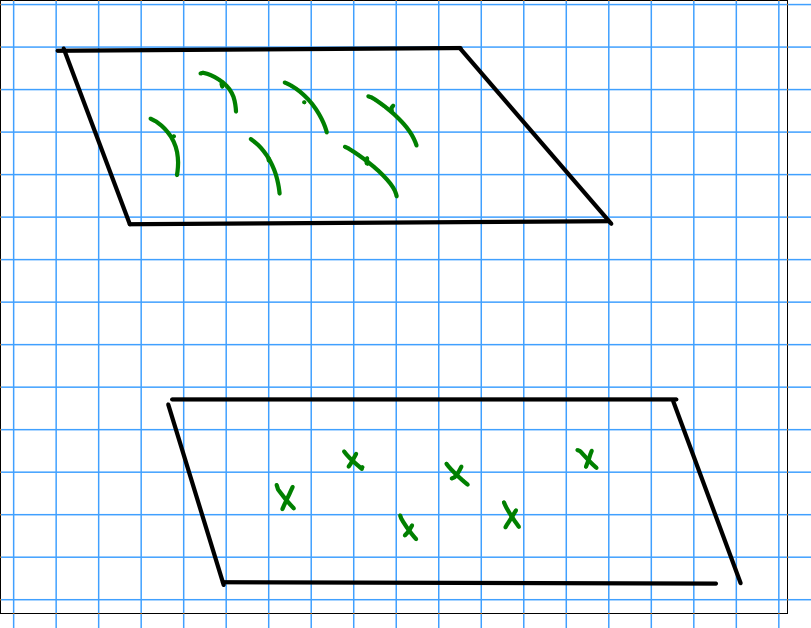
\includegraphics{figures/2020-02-18-13:07.png}
\caption{Image}
\end{figure}

Let \(\ell = \pi^*(\text{line})\), then a fact is that
\(3\ell - E_1 -\cdots - E_6\) (where \(E_i\) are the curves about the
\(p_i\)) is very ample and embeds \(X\) into \({\mathbb{P}}^3\) as a
cubic.

\end{fact}

\begin{fact}[Important fact 2]

Every smooth cubic surface \(X\) has \emph{precisely} 27 lines. Any 6
pairwise skew lines arise as \(E_1, \cdots, E_6\) as in the previous
construction.

\end{fact}

Take an \(X\) and a line \(L\subset X\). Consider any \(C\) in the
linear system \({\left\lvert {4H + 2L} \right\rvert}\). Fact:
\({\mathcal{O}}(4H + 2L)\) is very ample, so embeds into a big
projective space, and thus \(C\) is smooth and irreducible by Bertini.
Then the Hilbert polynomial of \(C\) is of the form \(at + b\) where
\(b = \chi({\mathcal{O}}_c)\), the Euler characteristic of the structure
sheaf of \(C\), and \(a = \deg C\). So we'll compute these. We have
\(\deg C = H \cdot C\) (intersection)
\(= H \cdot(4H + 2L) = 4H^2 + 2H\cdot L = 4\cdot 3 + 2 = 14\). The
intersections here correspond to taking hyperplane sections,
intersecting with \(X\) to get a curve, and counting intersection
points:

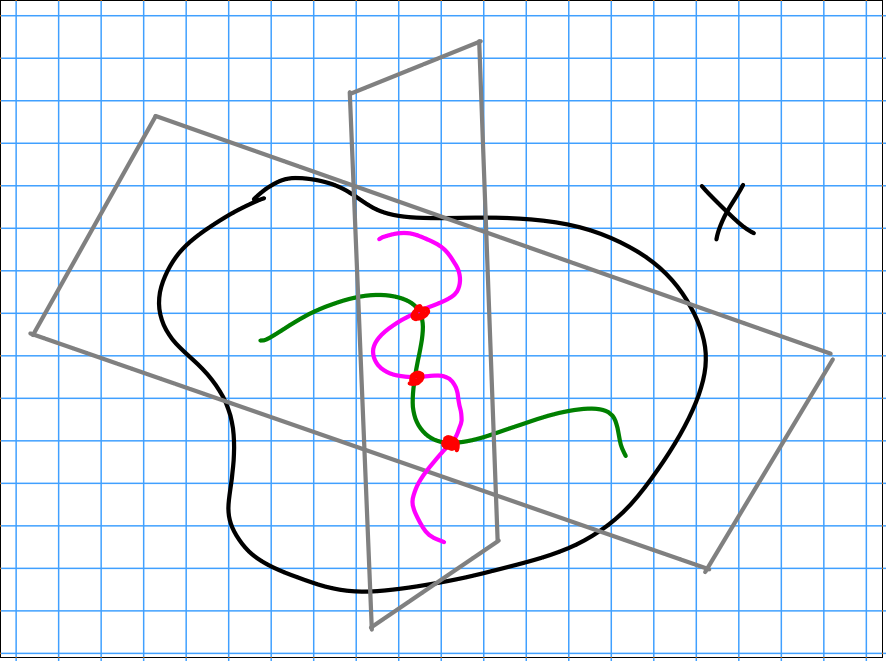
\includegraphics{figures/2020-02-18-13:14.png}\\

In general, for \(X\) a surface and \(C\subset X\) a smooth curve, then
\(\omega_C = \omega_X(C)\mathrel{\Big|}_C\). Since
\(X\subset {\mathbb{P}}^3\), we have
\begin{align*}
\omega_X 
&= \omega_{{\mathbb{P}}^3}(X) \mathrel{\Big|}_X \\
&= {\mathcal{O}}(-4) \oplus {\mathcal{O}}(3)\mathrel{\Big|}_X \\
&= {\mathcal{O}}_X(-1) \\
&= {\mathcal{O}}_X(-H)
.\end{align*}
We also have
\begin{align*}
\omega_C 
&= \omega_X(C)\mathrel{\Big|}_X  \\
&= { \left.{{ \qty{ {\mathcal{O}}_X(-H) \oplus {\mathcal{O}}_X(4H + 2L)}}} \right|_{{C}} } \\ \\
&\Downarrow \qquad \text{taking degrees} \\ \\
\deg \omega_C 
&= C\cdot(3H + 2L) \\
&= (4H+2L)(3H+2L) \\
&= 12H^2 + 14HL + 4L^2 \\
&= 36 + 14 + (-4) \\
&= 46
.\end{align*}
Since this equals \(2g(C) - 2\), we can conclude that the genus is given
by \(g(C) = 24\). Thus \(P\) is given by \(14t + (1-g) = 14t - 23\).

\begin{remark}

Good to know: moving a cubic surface moves the lines, you get a
monodromy action, and the Weyl group of \(E_6\) acts transitively so
lines look the same.

\end{remark}

\begin{claim}[1]

There is a flat family \(Z\subset {\mathbb{P}}^3_S\) with fiberwise
Hilbert polynomial \(P\) of cures of this form such that the image of
the map \(S \to \operatorname{Hilb}_{{\mathbb{P}}^3}^P\) has dimension
56.

\end{claim}

\begin{proof}[of claim]

We can compute the dimension of the space of smooth cubic surfaces,
since these live in
\({\mathbb{P}}H^0({\mathbb{P}}^3, {\mathcal{O}}(3))\), which has
dimension \({3+3\choose 3} -1 = 19\). Since there are 27 lines, the
dimension of the space of such cubics with a choices of a line is also
19. Choose a general \(C\) in the linear system
\({\left\lvert {4H + 2L} \right\rvert}\) will add
\(\dim {\left\lvert {4H + 2L} \right\rvert} = \dim {\mathbb{P}}H^0(x, {\mathcal{O}}_x(C))\).
We have an exact sequence
\begin{align*}
0 \to {\mathcal{O}}_X \to {\mathcal{O}}_X(C) \to {\mathcal{O}}_C(C) \to 0 \\
H^0\qty{ 0 \to {\mathcal{O}}_X \to {\mathcal{O}}_X(C) \to {\mathcal{O}}_C(C) \to 0 } \\
.\end{align*}

Since the first \(H^0\) vanishes (?) we get an isomorphism. By
Riemann-Roch, we have
\begin{align*}
\deg {\mathcal{O}}_C(C) = C^2 = (4H+2L)^2 = 16H^2 + 16 HL + 4L^2 = 64 - 4 = 60
.\end{align*}

We can also compute \(\chi({\mathcal{O}}_C(C)) = 60 - 23 = 37\). We have
\begin{align*}
h^0({\mathcal{O}}_C(C)) - h^1({\mathcal{O}}_C(C)) =  h^0({\mathcal{O}}_C(C)) - h^0(\omega_C(-C))) = 2(23) - 60 < 0
,\end{align*}
so there are no sections.

So \(\dim {\left\lvert {4H + 2L} \right\rvert} = 37\). Thus letting
\(S\) be the space of cubic surfaces \(X\), a line \(L\), and a general
\(C \in {\left\lvert {4H + 2L} \right\rvert}\), \(\dim S = 56\). We get
a map \(S \to \operatorname{Hilb}_{{\mathbb{P}}^3}^P\), and we need to
check that the fibers are 0-dimensional (so there are no redundancies).
We then just need that every such \(C\) lies on a unique cubic. Why does
this have to be the case? If \(C \subset X, X'\) then
\(C \subset X\cap X'\) is degree 14 curve sitting inside a degree 6
curve, which can't happen. Thus if \(H\) is a component of
\(\operatorname{Hilb}_{{\mathbb{P}}^3}^P\) containing the image of
\(S\), the \(\dim H \geq 56\).

\end{proof}

\begin{claim}[2]

For any \(C\) above, we have \(\dim T_C H = 57\).

\end{claim}

When the subscheme is smooth, we have an identification with sections of
the normal bundle \(T_C H = H^0(C, N_{C/{\mathbb{P}}^3})\). There's an
exact sequence

\begin{align*}
0 \to N_{C/X} = {\mathcal{O}}_C(C) \to N_{C/{\mathbb{P}}^3} \to N_{X/{\mathbb{P}}^3}\mathrel{\Big|}_C = {\mathcal{O}}_C(x)\mathrel{\Big|}_C = {\mathcal{O}}_C(3H)\mathrel{\Big|}_C \to 0
.\end{align*}

\begin{quote}
Note \(\omega_C = {\mathcal{O}}_C(3H + 2L)\).
\end{quote}

As we computed,
\begin{align*}
H^0({\mathcal{O}}_C(C)) &= 37 \\
H^1({\mathcal{O}}_C(C)) &= 0
.\end{align*}

So we need to understand the right-hand term
\(H^0({\mathcal{O}}_C(3H))\). By Serre duality, this equals
\(h^1(\omega_C(-3H)) = h^1({\mathcal{O}}_C(3L))\). We get an exact
sequence

\begin{align*}
0 \to {\mathcal{O}}_X(2L-C) \to {\mathcal{O}}_X(2L) \to {\mathcal{O}}_C(2L) \to 0
.\end{align*}

Taking homology, we have \(0\to 0 \to 1 \to 1 \to 0\) since
\(2L-C = -4H\). Computing degrees yields
\(h^0 ({\mathcal{O}}_C(3H)) = 20\). Thus the original exact sequence
yields
\begin{align*}
0 \to 37 \to ? \to 20 \to 0
,\end{align*}
so \(? = 57\) and thus \(\dim N_{C/{\mathbb{P}}^3} = 57\).

\begin{claim}[3]

\begin{align*}
\dim H = 56
.\end{align*}

\end{claim}

\hypertarget{proof-that-the-dimension-is-56}{%
\subsubsection{Proof That the Dimension is
56}\label{proof-that-the-dimension-is-56}}

Suppose otherwise. Then we have a family over \(H^\mathrm{red}\) of
\emph{smooth} curves, where \(f(S) \subset H^\mathrm{red}\), where the
generic element is not on a cubic or any lower degree surface. Let
\(C'\) be a generic fiber. Then \(C'\) lies on a pencil of quartics,
i.e.~2 linearly independent quartics. Let \(I = I_{C'}\) be the ideal of
this curve in \({\mathbb{P}}^3\), there is a SES
\begin{align*}
0\to I(4) \to {\mathcal{O}}(4) \to {\mathcal{O}}_C(4) \to 0
.\end{align*}
It can be shown that \(\dim H^0(I(4)) \geq 2\).

\begin{fact}

A generic quartic in this pencil is \emph{smooth} (can be argued because
of low degree and smoothness).

\end{fact}

We can compute the dimension of quartics, which is
\({4+3 \choose 3} - 1 = 35 - 1 = 34\). The dimension of \(C'\)s lying on
a fixed quartic is \(24\). But then the dimension of the image in the
Hilbert scheme is at most \(24 + 34 - 1 = 57\). It can be shown that the
picard rank of such a quartic is 1, generated by \({\mathcal{O}}(1)\),
so this is a \emph{strict} inequality, which is a contradiction since
\(\dim \operatorname{Hilb}= 56\). This proves the theorem.

\begin{remark}

Use the fact that these curves are \(K3\) surfaces? Get the fact about
the generator of the Picard group from Hodge theory. So we can deform
curves a bit, but not construct an algebraic family that escapes a
particular cubic.

\end{remark}

\hypertarget{obstruction-and-deformation-tuesday-february-25th}{%
\section{Obstruction and Deformation (Tuesday February
25th)}\label{obstruction-and-deformation-tuesday-february-25th}}

Let \(k\) be a field, \(X_{_{/k}}\) projective, then the
\(k{\hbox{-}}\)points \(\operatorname{Hilb}_{X_{_{/k}}}^P(k)\)
corresponds to closed subschemes \(Z\subset X\) with hilbert polynomial
\(P_z = P\). Given a \(P\), we want to understand the local structure of
\(\operatorname{Hilb}_{X_{_{/k}}}^p\), i.e.~diagrams of the form

\begin{center}
\begin{tikzcd}
                                        &  &                                               &  & \operatorname{Hilb}_{X_{_{/k}}}^P \arrow[dd] \\
                                        &  &                                               &  &                          \\
\operatorname{Spec}(k) \arrow[rrrruu, "p"] \arrow[rr] &  & \operatorname{Spec}(A) \arrow[rruu, "?", dashed] \arrow[rr] &  & \operatorname{Spec}(k)                 \\
                                        &  &                                               &  &                          \\
                                        &  & A_{/k} \text{ Artinian local} \arrow[uu]         &  &
\end{tikzcd}
\end{center}

\begin{example}[?]

For \(A = k[\varepsilon]\), the set of extensions is the Zariski tangent
space.

\end{example}

\begin{definition}[Category of Artinian Algebras]

Let \((\operatorname{Art}_{/k})\) be the category of local Artinian
\(k{\hbox{-}}\)algebras with local residue field \(k\).

\end{definition}

Note that these will be the types of algebras appearing in the above
diagrams.

\begin{remark}

This category has fiber coproducts, i.e.~there are pushouts:

\begin{center}
\begin{tikzcd}
C \arrow[dd] \arrow[rr] &  & A \arrow[dd, dashed] \\
                        &  &                      \\
B \arrow[rr, dashed]    &  & A \otimes_C B
\end{tikzcd}
\end{center}

There are also fibered products,

\begin{center}
\begin{tikzcd}
A \times_C B \arrow[rr, dashed] \arrow[dd, dashed] &  & B \arrow[dd] \\
                                                  &  &              \\
A \arrow[rr]                                       &  & C
\end{tikzcd}
\end{center}

Here,
\(A \times_C B \coloneqq\left\{{(a, b) {~\mathrel{\Big|}~}f(a) = g(b)}\right\} \subset A\times B\).

\end{remark}

\begin{example}[?]

If \(A = B = k[\varepsilon]/(\varepsilon^2)\) and \(C = k\), then
\(A\times_C B = k[\varepsilon_1, \varepsilon_2]/(\varepsilon_1, \varepsilon_2)^2\)

Note that on the \(\operatorname{Spec}\) side, these should be viewed as
\begin{align*}
\operatorname{Spec}(A) {\coprod}_{\operatorname{Spec}(C)} \operatorname{Spec}(B) = \operatorname{Spec}(A\times_C B)
.\end{align*}

\end{example}

\begin{definition}[Deformation Functor (Preliminary Definition)]

A \emph{deformation functor} is a functor
\(F: (\operatorname{Art}_{/k}) \to {\operatorname{Set}}\) such that
\(F(k) = {\{\operatorname{pt}\}}\) is a singleton.

\end{definition}

\begin{example}[?]

Let \(X_{_{/k}}\) be any scheme and let \(x\in X(k)\) be a
\(k{\hbox{-}}\)point. We can consider the deformation functor \(F\) such
that \(F(A)\) is the set of extensions \(f\) of the following form:

\begin{center}
\begin{tikzcd}
                                          &  &                                               &  & X \arrow[dd] \\
                                          &  &                                               &  &              \\
\operatorname{Spec}(k) \arrow[rrrruu, "x"] \arrow[rr, hook] &  & \operatorname{Spec}(A) \arrow[rruu, "f", dashed] \arrow[rr] &  & \operatorname{Spec}(k)
\end{tikzcd}
\end{center}

If \(A' \to A\) is a morphism, then we define \(F(A') \to F(A)\) is
defined because we can precompose to fill in the following diagram

\begin{center}
\begin{tikzcd}
                                    &  &                                                            &  &                                                       &  &  &  & X \arrow[ddd] \\
                                    &  &                                                            &  &                                                       &  &  &  &               \\
                                    &  &                                                            &  &                                                       &  &  &  &               \\
\operatorname{Spec}(k) \arrow[rrd] \arrow[rrrrrrrruuu] &  &                                                            &  &                                                       &  &  &  & \operatorname{Spec}(k)      \\
                                    &  & \operatorname{Spec}(A) \arrow[rr] \arrow[rrrrrruuuu, "\exists \tilde f"] &  & \operatorname{Spec}(A') \arrow[rrrru] \arrow[rrrruuuu, "f", dashed] &  &  &  &
\end{tikzcd}
\end{center}

So this is indeed a deformation functor.

\end{example}

\begin{example}[a motivating example]

The Zariski tangent space on the nodal cubic doesn't ``see'' the two
branches, so we allow ``second order'' tangent vectors.

\end{example}

We can consider parametrizing the functors above as \(F_{X, x}(A)\),
which is isomorphic to
\(F_{\operatorname{Spec}({\mathcal{O}}_x)_{X, x}}\) and further
isomorphic to
\(F_{\operatorname{Spec}\widehat{{\mathcal{O}}_x}_{x, X} }\). This is
because for Artinian algebras, we have maps
\begin{align*}
\operatorname{Spec}({\mathcal{O}}_{x, X})/{\mathfrak{m}}^N \to \operatorname{Spec}{\mathcal{O}}_{X, x} \to X
.\end{align*}

\begin{remark}

\(\widehat{ {\mathcal{O}}}_{X, x}\) will be determined by \(F_{X, x}\).

\end{remark}

\begin{example}[?]

Consider \(y^2 = x^2(x+1)\), and think about solving this over
\(k[t]/t^n\) with solutions equivalent to \((0, 0) \pmod t\).

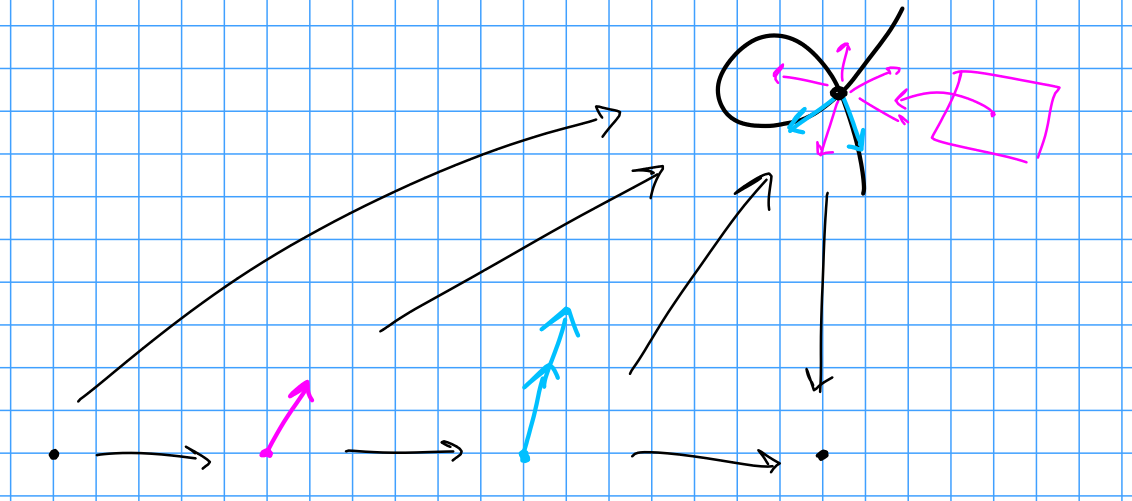
\includegraphics{figures/2020-02-25-13:20.png}\\

Note that the `second order' tangent vector comes from
\(\operatorname{Spec}k[t]/t^3\).

We can write \(F_{X, x}(A) = \pi^{-1}(x)\) where
\begin{align*}
\hom_{{\operatorname{Sch}}_{/k}}(\operatorname{Spec}k, X) \xrightarrow{\pi} \hom_{{\operatorname{Sch}}_{/k}}(\operatorname{Spec}k, x) \ni x
.\end{align*}
Thus
\begin{align*}
F_{X, x}(A) = \hom_{{\operatorname{Sch}}_{/k}}(\operatorname{Spec}A, \operatorname{Spec}{\mathcal{O}}_{x, X}) = \hom_{k{\hbox{-}}\mathrm{Alg}}(\widehat{{\mathcal{O}}}_{X, x}, A)
.\end{align*}

\end{example}

\begin{example}[?]

Given any local \(k{\hbox{-}}\)algebra \(R\), we can consider

\begin{align*}
h_R: (\operatorname{Art}_{/k}) &\to {\operatorname{Set}}\\
A &\mapsto \hom(R, A)
.\end{align*}

and

\begin{align*}
h_{\operatorname{Spec}R}: (\operatorname{Art}{\operatorname{Sch}}_{/k})^{\operatorname{op}}\to {\operatorname{Set}}\\
\operatorname{Spec}(A) &\mapsto \hom(\operatorname{Spec}A, \operatorname{Spec}R)
.\end{align*}

\end{example}

\begin{definition}[Representable Deformation]

A deformation \(F\) is \textbf{representable} if it is of the form
\(h_R\) as above for some \(R \in \operatorname{Art}_{/k}\).

\end{definition}

\begin{remark}

There is a Yoneda Lemma for \(A\in \operatorname{Art}_{/k}\),
\begin{align*}
\hom_{\mathrm{Fun}}(h_A, F) = F(A)
.\end{align*}

We are thus looking for things that are representable in a larger
category, which restrict.

\end{remark}

\begin{definition}[Pro-Representability]

A deformation functor is \emph{pro-representable} if it is of the form
\(h_R\) for \(R\) a complete local \(k{\hbox{-}}\)algebra (i.e.~a limit
of Artinian local \(k{\hbox{-}}\)algebras).

\end{definition}

\begin{remark}

We will see that there are simple criteria for a deformation functor to
be pro-representable. This will eventually give us the complete local
ring, which will give us the scheme representing the functor we want.

\end{remark}

\begin{remark}

It is difficult to understand even \(F_{X, x}(A)\) directly, but it's
easier to understand small extensions.

\end{remark}

\begin{definition}[Small Extensions]

A \emph{small extension} is a SES of Artinian \(k{\hbox{-}}\)algebras of
the form
\begin{align*}
0 \to J \to A' \to A \to 0
.\end{align*}
such that \(J\) is annihilated by the maximal ideal fo \(A'\).

\end{definition}

\begin{lemma}[?]

Given any quotient \(B\to A \to 0\) of Artinian \(k{\hbox{-}}\)algebras,
there is a sequence of small extensions (quotients):

\begin{center}
\begin{tikzcd}
0                                          &  &                  &  &        &  &                          \\
                                        &  &                  &  &        &  &                          \\
B_0 \arrow[uu]                             &  & B_1 \arrow[lluu] &  & \cdots &  & B_n = A \arrow[lllllluu] \\
                                        &  &                  &  &        &  &                          \\
B \arrow[uu] \arrow[rruu] \arrow[rrrrrruu] &  &                  &  &        &  &
\end{tikzcd}
\end{center}

This yields

\begin{center}
\begin{tikzcd}
\operatorname{Spec}A \arrow[rrrr, hook] \arrow[rrrrdddddd, Rightarrow] &  &  &  & \operatorname{Spec}B                    \\
                                                        &  &  &  &                            \\
                                                        &  &  &  & \operatorname{Spec}B_0 \arrow[uu, hook] \\
                                                        &  &  &  &                            \\
                                                        &  &  &  & \vdots \arrow[uu, hook]    \\
                                                        &  &  &  &                            \\
                                                        &  &  &  & \operatorname{Spec}B_n \arrow[uu, hook]
\end{tikzcd}
\end{center}

where the \(\operatorname{Spec}B_i\) are all small.

\end{lemma}

\begin{remark}

In most cases, extending deformations over small extensions is easy.

\end{remark}

\hypertarget{first-example-of-deformation-and-obstruction-spaces}{%
\subsection{First Example of Deformation and Obstruction
Spaces}\label{first-example-of-deformation-and-obstruction-spaces}}

Suppose
\(k=\mkern 1.5mu\overline{\mkern-1.5muk\mkern-1.5mu}\mkern 1.5mu\) and
let \(X_{_{/k}}\) be connected. We have a picard functor
\begin{align*}
{\operatorname{Pic}}_{X_{_{/k}}}: ({\operatorname{Sch}}_{/k})^{\operatorname{op}}&\to {\operatorname{Set}}\\
S &\mapsto {\operatorname{Pic}}(X_S) / {\operatorname{Pic}}(S)
.\end{align*}
If we take a point \(x\in {\operatorname{Pic}}_{X_{_{/k}}}(k)\), which
is equivalent to line bundles on \(X\) up to equivalence, we obtain a
deformation functor
\begin{align*}
F \coloneqq F_{{\operatorname{Pic}}_{ X_{_{/k}}, x  }} &\to {\operatorname{Set}}\\
A \mapsto \pi^{-1}(x)
\end{align*}
where
\begin{align*}
\pi: {\operatorname{Pic}}_{X_{_{/k}}}(\operatorname{Spec}A) &\to {\operatorname{Pic}}_{X_{_{/k}}} (\operatorname{Spec}k) \\
\pi^{-1}(x) &\mapsto x
.\end{align*}

This is given by taking a line bundle on the thickening and restricting
to a closed point. Thus the functor is given by sending \(A\) to the set
of line bundles on \(X_A\) which restrict to \(X_x\). That is,
\(F(A) \subset {\operatorname{Pic}}_{X_{_{/k}}}(\operatorname{Spec}A)\)
which restrict to \(x\). So just pick the subspace
\({\operatorname{Pic}}(X_A)\) (base changing to \(A\)) which restrict.
There is a natural identification of
\({\operatorname{Pic}}(X_A) = H^1(X_A, {\mathcal{O}}_{X_A}^*)\). If
\begin{align*}
0\to J \to A' \to A \to 0
.\end{align*}
is a thickening of Artinian \(k{\hbox{-}}\)algebras, there is a
restriction map of invertible functions
\begin{align*}
{\mathcal{O}}_{X_A}^* \to {\mathcal{O}}_{X_A'}^* \to 0
.\end{align*}
which is surjective since the map on structure sheaves is surjective and
its a nilpotent extension. The kernel is then just
\({\mathcal{O}}_{X_{A'}} \otimes J\). If this is a small extension, we
get a SES
\begin{align*}
0 \to {\mathcal{O}}_X \otimes J \to {\mathcal{O}}_{X_{A'}}^* \to {\mathcal{O}}_{x_A}^* \to 0
.\end{align*}
Taking the LES in cohomology, we obtain
\begin{align*}
H^1 {\mathcal{O}}_X \otimes J \to H^1 {\mathcal{O}}_{X_{A'}}^* \to H^1{\mathcal{O}}_{x_A}^* \to H^0 {\mathcal{O}}_X \otimes J
.\end{align*}
Thus there is an obstruction class in \(H^2\), and the ambiguity is
detected by \(H^1\). Thus \(H^1\) is referred to as the
\textbf{deformation space}, since it counts the extensions, and \(H^2\)
is the \textbf{obstruction space}.

\hypertarget{deformation-theory-thursday-february-27th}{%
\section{Deformation Theory (Thursday February
27th)}\label{deformation-theory-thursday-february-27th}}

Big picture idea: We have moduli functors, such as

\begin{align*}
F_{S'}: ({\operatorname{Sch}}_{/k})^{\operatorname{op}}&\to {\operatorname{Set}}\\
\operatorname{Hilb}: S &\to \text{flat subschemes of } X_S \\
{\operatorname{Pic}}: S &\to {\operatorname{Pic}}(X_S)/{\operatorname{Pic}}(S) \\
\mathrm{Def}: S &\to \text{flat families } / S,~ \text{smooth, finite, of genus } g
.\end{align*}

\begin{definition}[Deformation Theory]

Choose a point \(f\) the scheme representing \(F_{S'}\) with
\(\xi_0 \in F_{gl}(\operatorname{Spec}K)\). Define

\begin{align*}
F_{\text{loc}}: (\text{Artinian local schemes} / K)^{\operatorname{op}}\to {\operatorname{Set}}
.\end{align*}

\begin{center}
\begin{tikzcd}
\operatorname{Spec}(K) \arrow[rr, "i", hook] &  & \operatorname{Spec}(A) \arrow[rr] &  & F(i)^{-1}(\xi_0) \arrow[rr] &  & F_{gr}(\operatorname{Spec}K) \arrow[dd, "F(i)"] \\
                               &  &                     &  &                            &  &                                    \\
                               &  &                     &  &                            &  & F_{gl}(\operatorname{Spec}K)
\end{tikzcd}
\end{center}

\end{definition}

\begin{definition}[Deformation Functors]

Let \(F: (\operatorname{Art}_{/k}) \to {\operatorname{Set}}\) where
\(F(k)\) is a point. Denote \(\widehat{\operatorname{Art}}_{/k}\) the
set of complete local \(k{\hbox{-}}\)algebras. Since
\(\operatorname{Art}_{/k} \subset \widehat{\operatorname{Art}} / k\), we
can make extensions \(\widehat{F}\) by just taking limits:

\begin{center}
\begin{tikzcd}
                                & \operatorname{Art}_{/k} \arrow[rrr, "F"]                         &  &  & {\operatorname{Set}}\\
                                &                                                 &  &  &      \\
\lim_{\leftarrow} R/{\mathfrak{m}}_R^n = R \in & \widehat{\operatorname{Art}}_{/k} \arrow[uu] \arrow[rrruu, "\widehat{F}"] &  &  &
\end{tikzcd}
\end{center}

where we define
\begin{align*}
\widehat{F}(R) \coloneqq\varprojlim F(R/{\mathfrak{m}}_R^n)
.\end{align*}

\end{definition}

\begin{question}

When is \(F\) pro-representable, which happens iff \(\widehat{F}\) is
representable? In particular, we want
\(h_R \xrightarrow{\cong} \widehat{F}\) for
\(R\in \widehat{\operatorname{Art}}_{/k}\), so
\begin{align*}
h_R = \hom_{\widehat{\operatorname{Art}}_{/k}}(R, {\,\cdot\,}) = \hom_{?}({\,\cdot\,}, \operatorname{Spec}k)
.\end{align*}

\end{question}

\begin{example}[?]

Let \(F_{\text{gl}} = \operatorname{Hilb}_{X_{_{/k}}}^p\), which is
represented by \(H_{/k}\). Then .
\begin{align*}
\xi_0 = F_{\text{gl}}(k) = H(k) = \left\{{Z\subset X {~\mathrel{\Big|}~}P_z = f}\right\}
.\end{align*}
Then \(F_{\text{loc} }\) is representable by
\(\widehat{{\mathcal{O}}}_{H/\xi_0}\).

\end{example}

\begin{definition}[Thickening]

Given an Artinian \(k{\hbox{-}}\)algebra
\(A \in \operatorname{Art}_{/k}\), a \emph{thickening} is an
\(A' \in \operatorname{Art}_{/k}\) such that
\(0 \to J \to A' \to A \to 0\), so
\(\operatorname{Spec}A \hookrightarrow\operatorname{Spec}A'\).

\end{definition}

\begin{definition}[Small Thickening]

A \textbf{small thickening} is a thickening such that
\(0 = {\mathfrak{m}}_{A'} J\), so \(J\) becomes a module for the residue
field, and \(\dim_k J = 1\).

\end{definition}

\begin{lemma}[?]

Any thickening of \(A\), say \(B\to A\), fits into a diagram:

\begin{center}
\begin{tikzcd}
&  &                                      &  & 0                        &  &                                     &  &   \\
&  &                                      &  &                          &  &                                     &  &   \\
&  & J \arrow[rr]                         &  & A' \arrow[uu] \arrow[rr] &  & A \arrow[dd, Rightarrow] \arrow[rr] &  & 0 \\
&  &                                      &  &                          &  &                                     &  &   \\
0 \arrow[rr] &  & I \arrow[rr] \arrow[uu]              &  & B \arrow[uu] \arrow[rr]  &  & A \arrow[rr]                        &  & 0 \\
&  &                                      &  &                          &  &                                     &  &   \\
&  & I' \arrow[rr, Rightarrow] \arrow[uu] &  & I' \arrow[uu]            &  &                                     &  &   \\
&  &                                      &  &                          &  &                                     &  &   \\
&  & 0 \arrow[uu]                         &  & 0 \arrow[uu]             &  &                                     &  &
\end{tikzcd}
\end{center}

\end{lemma}

\begin{proof}[of lemma]

We just need \(I' \subset I\) with
\({\mathfrak{m}}_S I \subset J' \subset I \iff J {\mathfrak{m}}_B = 0\).
Choose \(J'\) to be a preimage of a codimension 1 vector space in
\(I/{\mathfrak{m}}_B I\). Thus \(J = I/I'\) is 1-dimensional.

\end{proof}

Thus any thickening \(A\) can be obtained by a sequence of small
thickenings. By the lemma, in principle \(F\) and thus \(\widehat{F}\)
are determined by their behavior under small extensions.

\hypertarget{example}{%
\subsubsection{Example}\label{example}}

Consider \({\operatorname{Pic}}\), fix \(X_{_{/k}}\), start with a line
bundle
\(L_0 \in {\operatorname{Pic}}(x) /{\operatorname{Pic}}(k) = {\operatorname{Pic}}(x)\)
and the deformation functor \(F(A)\) being the set of line bundles \(L\)
on \(X_A\)with \({\left.{{L}} \right|_{{x}} } \cong L_0\), modulo
isomorphism. Note that this yields a diagram

\begin{center}
\begin{tikzcd}
x \arrow[rr] \arrow[dd, hook] &  & k \arrow[dd, "\text{unique closed point}"] \\
                              &  &                                            \\
X_A \arrow[rr]                &  & \operatorname{Spec}A
\end{tikzcd}
\end{center}

This is equal to \((I_x)^{-1}(L_0)\), where
\({\operatorname{Pic}}(X_a) \xrightarrow{I_x} {\operatorname{Pic}}(x)\).
If
\begin{align*}
0 \to J \to A' \to A \to 0
.\end{align*}
is a small thickening, we can identify

\begin{center}
\begin{tikzcd}
0 \arrow[rr] &  & J \otimes_x {\mathcal{O}}_{x} \cong {\mathcal{O}}_x \arrow[rr] &  & {\mathcal{O}}_{X_{A'}} \arrow[rr]                    &  & {\mathcal{O}}_{X_{A}} \arrow[rr]   &  & 0 &  & \\
          &  &                                            &  &                                            &  &                          &  &   &  &\in\text{AbSheaves}                      \\
0 \arrow[rr] &  & {\mathcal{O}}_x \arrow[rr, "f\mapsto 1+f"]                           &  & {\mathcal{O}}_{X_{A'}}^* \arrow[rr] \arrow[uu, hook] &  & {\mathcal{O}}_{X_{A}}^* \arrow[rr] &  & 0 &  &
\end{tikzcd}
\end{center}

This yields a LES

\begin{center}
\begin{tikzcd}[column sep=tiny]
0 \arrow[rr]            &  & {H^0(X, {\mathcal{O}}_x) = k} \arrow[rr] &  & {H^0(X_{A'}, {\mathcal{O}}_{x_{A'}}^*) = {A'}^*} \arrow[rr]                                     &  & {H^0(X_{A'}, {\mathcal{O}}_{x_{A}}^*) = A^*} \arrow[lllldd] \arrow[rr]         &  & \therefore 0 \\
                        &  &                                &  &                                                                                       &  &                                                                      &  &              \\
\therefore 0 \arrow[rr] &  & {H^1(X, {\mathcal{O}}_{x})} \arrow[rr]   &  & {H^1(X_{A'}, {\mathcal{O}}_{x_{A'}}^*) = {\operatorname{Pic}}(X_{A'})} \arrow[rr, "\scriptsize\text{restriction to } X_A", outer sep=1em] &  & {H^1(X_{A}, {\mathcal{O}}_{x_{A}}^*) = {\operatorname{Pic}}(X_A)} \arrow[lllldd, "\text{obs}"] &  &              \\
                        &  &                                &  &                                                                                       &  &                                                                      &  &              \\
&  & {H^2(X, {\mathcal{O}}_x)} \ar[rr]                & &\cdots                                                                                        &  &                                                                      &  &
\end{tikzcd}
\end{center}

\begin{remark}

To understand \(F\) on small extensions, we're interested in

\begin{enumerate}
\def\labelenumi{\arabic{enumi}.}
\item
  Given \(L \in F_{\text{loc}}(A)\), i.e.~\(L\) on \(X_A\) restricting
  to \(L_0\), when does it extend to \(L' \in F_{\text{loc}}(A')\)?
  I.e., does there exist an \(L'\) on \(X_{A'}\) restricting to \(L\)?
\item
  Provided such an extension \(L'\) exists, how many are there, and what
  is the structure of the space of extensions?
\end{enumerate}

\end{remark}

\begin{question}

We have an \(L\in {\operatorname{Pic}}(X_A)\), when does it extend?

\end{question}

By exactness, \(L'\) exists iff
\(\text{obs}(L) = 0\in H^2(X, {\mathcal{O}}_x)\), which answers 1. To
answer 2, \((I_x)^{-1}(L)\) is the set of extensions of \(L\), which is
a torsor under \(H^1(x, {\mathcal{O}}_x)\). Note that these are fixed
\(k{\hbox{-}}\)vector spaces.

\begin{remark}

\(H^1(X, {\mathcal{O}}_x)\) is interpreted as the \textbf{tangent space}
of the functor \(F\), i.e.~\(F_{\text{loc}}(K[\varepsilon])\). Note that
if \(X\) is projective, line bundles can be unobstructed without the
group itself being zero.

\end{remark}

For (3), just play with \(A = k[\varepsilon]\), which yields
\(0 \to k \xrightarrow{\varepsilon} k[\varepsilon] \to k \to 0\), then

\begin{center}
\begin{tikzcd}
0 \arrow[rr] &  & {H^1(X, {\mathcal{O}}_x)} \arrow[rr] &  & {H^1(X_{k[\varepsilon]}, {\mathcal{O}}_{k[\varepsilon]}^*)} \arrow[rr, "I_x"] &  & {H^1(X, {\mathcal{O}}_x^*)} \arrow[ll, bend right=49] \\
             &  &                            &  & {(I_x)^{-1}(L_0) \in {\operatorname{Pic}}(X_{k[\varepsilon]})}                &  & L_0 \in {\operatorname{Pic}}(x)
\end{tikzcd}
\end{center}

i.e., there is a canonical trivial extension \(L_0[\varepsilon]\).

\begin{example}[?]

Let \(X \supset Z_0 \in \operatorname{Hilb}_{X_{_{/k}}}(k)\), we
computed
\begin{align*}
T_{Z_0} \operatorname{Hilb}_{X_{_{/k}}} =  \hom_{{\mathcal{O}}_x}(I_{Z_0}, {\mathcal{O}}_z)
.\end{align*}
We took \(Z_0 \subset X\) and extended to
\(Z' \subset X_{k[\varepsilon]}\) by base change. In this case,
\(F_{\text{loc}}(A)\) was the set of \(Z'\subset X_A\) which are flat
over \(A\), such that base-changing
\(Z' \times_{\operatorname{Spec}A} \operatorname{Spec}k \cong Z\). This
was the same as looking at the preimage restricted to the closed point,
\begin{align*}
\operatorname{Hilb}_{X_{_{/k}}}(A) \xrightarrow{i^*} \operatorname{Hilb}_{X_{_{/k}}}(k) \\
(i^*)^{-1}(z_0) \mapsfrom z_0
.\end{align*}
Recall how we did the thickening: we had \(0 \to J \to A' \to A \to 0\)
with \(J^2 = 0\), along with \(F\) on \(X_A\) which is flat over \(A\)
with \(X_{_{/k}}\) projective, and finally an \(F'\) on \(X_{A'}\)
restricting to \(F\). The criterion we had was \(F'\) was flat over
\(A'\) iff \(0 \to J\otimes_{A'} F' \to F'\), i.e.~this is injective.
Suppose \(z\in F_{\text{loc}}(A)\) and an extension
\(z' \in F_{\text{loc}}(A')\). By tensoring the two exact sequences
here, we get an exact grid:

\begin{center}
\begin{tikzcd}
0 \arrow[rr] \arrow[dd] &             & I_{Z'} \arrow[rr]             &  & {\mathcal{O}}_{X_{A'}} \arrow[rr]            &  & {\mathcal{O}}_{Z'} \arrow[rr]            &   & 0 \\
                      &             & 0 \arrow[d]                   &  & 0 \arrow[d]                        &  & 0 \arrow[d]                    &   &   \\
J \arrow[dd]            & 0 \arrow[r] & I_{Z_0} \arrow[dd] \arrow[rr] &  & {\mathcal{O}}_X \arrow[dd] \arrow[rr]        &  & {\mathcal{O}}_{Z_0} \arrow[dd] \arrow[r] & 0 &   \\
                      &             &                               &  &                                    &  &                                &   &   \\
A' \arrow[dd]           & 0 \arrow[r] & I_{Z'} \arrow[rr] \arrow[dd]  &  & {\mathcal{O}}_{X_{A'}} \arrow[rr] \arrow[dd] &  & {\mathcal{O}}_{Z'} \arrow[dd] \arrow[r]  & 0 &   \\
                      &             &                               &  &                                    &  &                                &   &   \\
A \arrow[dd]            & 0 \arrow[r] & I_Z \arrow[d] \arrow[rr]      &  & {\mathcal{O}}_{X_A} \arrow[rr] \arrow[d]     &  & {\mathcal{O}}_Z \arrow[d] \arrow[r]      & 0 &   \\
                      &             & 0                             &  & 0                                  &  & 0                              &   &   \\
0                       &             &                               &  &                                    &  &                                &   &
\end{tikzcd}
\end{center}

The space of extension should be a torsor under
\(\hom_{{\mathcal{O}}_X}(I_{Z_0}, {\mathcal{O}}_{Z_0})\), which we want
to think of as \(\hom_{{\mathcal{O}}_X}(I_{Z_0}, {\mathcal{O}}_{Z_0})\).
Picking a \(\phi\) in this hom space, we want to take an extension
\(I_{Z'} \xrightarrow{\phi} I_{Z''}\).

\end{example}

\begin{quote}
We'll cover how to make this extension next time.
\end{quote}

\hypertarget{tuesday-march-31st}{%
\section{Tuesday March 31st}\label{tuesday-march-31st}}

See notes on Ben's website. We'll review where we were.

\hypertarget{deformation-theory}{%
\subsection{Deformation Theory}\label{deformation-theory}}

We want to represent certain moduli functors by schemes. If we know a
functor is representable, it's easier to understand the deformation
theory of it and still retain a lot of geometric information. The
representability of deformation is much easier to show. We're
considering functors
\(F: \operatorname{Art}_{/k} \to {\operatorname{Set}}\).

\begin{example}[?]

The Hilbert functor
\begin{align*}
\operatorname{Hilb}_{X_{_{/k}}} ({\operatorname{Sch}}_{/k})^{\operatorname{op}}\to {\operatorname{Set}}\\
S \mapsto \left\{{ Z  \subset  X \times S \text{ flat over } S}\right\}
.\end{align*}

This yields
\begin{align*}
F: \operatorname{Art}_{/k} \to {\operatorname{Set}}\\
???
.\end{align*}

\end{example}

\begin{figure}
\centering
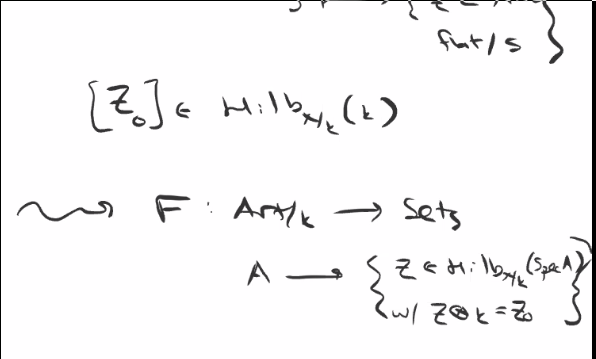
\includegraphics{figures/2020-03-31-12:44.png}
\caption{Image}
\end{figure}

Recall that we're interested in pro-representability, where
\(\widehat{F}(R) = \varprojlim F(R\mu_R^n)\) is given by a lift of the
form

\begin{center}
\begin{tikzcd}
\operatorname{Art}_{/k} 
  \ar[r, "F"] 
& {\operatorname{Set}}
\\
\widehat{\operatorname{Art}_{/k}}
  \ar[u, hook] 
  \ar[ur, "\widehat{F}"']
&
\end{tikzcd}
\end{center}

\begin{question}

Is \(\widehat{F}\) representable, i.e.~is \(F\) pro-representable?

\end{question}

\begin{example}[?]

The \(F\) in the previous example is pro-representable by
\(\widehat{F} = \hom({\mathcal{O}}_{\operatorname{Hilb}, z_0}, {\,\cdot\,})\).

\end{example}

\begin{definition}[Pro-Representable Hull]

\(F\) has a \emph{pro-representable hull} iff there is a formally smooth
map \(h_R \to F\).

\end{definition}

\begin{question}

Does \(F\) have a pro-representable hull?

\end{question}

Recall that a map of functors on artinian \(k{\hbox{-}}\)algebras is
\textbf{formally smooth} if it can be lifted through nilpotent
thickenings. That is, for
\(F, G: \operatorname{Art}_{/k} \to {\operatorname{Set}}\), \(F \to G\)
is \emph{formally smooth} if for any thickening
\(A' \twoheadrightarrow A\), we have

\begin{center}
\begin{tikzcd}
& 
& F 
  \ar[d] 
\\
h_{A} 
  \ar[rru] 
  \ar[r] 
& h_{A'} 
  \ar[ru, dotted] 
  \ar[r] 
& G
\\
  \operatorname{Spec}A 
  \ar[u, equal] 
  \ar[r] 
& \operatorname{Spec}A' 
  \ar[u, equal] 
  \ar[r] 
& G
  \ar[u, equal]
\end{tikzcd}
\end{center}

We proved for \(R, A\) finite type over \(k\),
\(\operatorname{Spec}R \to \operatorname{Spec}A\) smooth is formally
smooth. Given a complete local \(k{\hbox{-}}\)algebra \(R\) and a
section \(\xi \in \widehat{F}(R)\), we make the following definitions:

\begin{definition}[Versal, Miniversal, Universal]

The pair \((R, \xi)\) is

\begin{itemize}
\item
  \emph{Versal} for \(F\) iff \(h_R \xrightarrow{\xi} F\) is formally
  smooth.\footnote{Not a unique map, but still a pullback}
\item
  \emph{Miniversal} for \(F\) iff versal and an isomorphism on Zariski
  tangent spaces.
\item
  \emph{Universal} for \(F\) if \(h_R \xrightarrow{\cong} F\) is an
  isomorphism, i.e.~\(h_R\) pro-represents \(F\).

  \begin{itemize}
  \tightlist
  \item
    Pullback by a unique map
  \end{itemize}
\end{itemize}

\end{definition}

\begin{remark}

Note that \textbf{versal} means that any formal section \((s, \eta)\)
where \(\eta \in \widehat{F}(s)\) comes from pullback, i.e there exists
a map
\begin{align*}
R &\to S \\
\widehat{F}(R) &\to \widehat{F}(s) \\
\xi &\mapsto \eta
.\end{align*}

\textbf{Miniversal} means adds that the derivative is uniquely
determined, and universal means that \(R\to S\) is unique.

\end{remark}

\begin{definition}[Obstruction Theory]

An \textbf{obstruction theory} for \(F\) is the data of
\(\mathrm{def}(F), \mathrm{obs}(F)\) which are finite-dimensional
\(k{\hbox{-}}\)vector spaces, along with a functorial assignment of the
following form:
\begin{align*}
(A' \twoheadrightarrow A) \quad \text{a small thickening } \mapsto \\
\mathrm{def}(F) {\circlearrowleft}F(A') \to F(A) \xrightarrow{\mathrm{obs}} \mathrm{obs}(F)
\end{align*}
that is exact\footnote{Recall that right-exactness was a transitive
  action.} and if \(A=k\), it is exact on the left (so the action was
faithful on nonempty fibers).

\end{definition}

\begin{example}[?]

We have
\begin{align*}
{\operatorname{Pic}}_{X_{/k}} : ({\operatorname{Sch}}_{/k})^{\operatorname{op}}&\to {\operatorname{Set}}\\
S &\mapsto {\operatorname{Pic}}(X\times X) / {\operatorname{Pic}}(S)
.\end{align*}

This yields
\begin{align*}
F: \operatorname{Art}_{/k} \to {\operatorname{Set}}\\
A \mapsto L\in {\operatorname{Pic}}(X_A),~ L\otimes k \cong L_0
\end{align*}
where \(X_{_{/k}}\) is proper and irreducible. Then \(F\) has an
obstruction theory with \(\mathrm{def}(F) = H^1({\mathcal{O}}_x)\) and
\(\mathrm{obs}(F) = H^2({\mathcal{O}}_x)\). The key was to look at the
LES of
\begin{align*}
0 \to {\mathcal{O}}_x \to {\mathcal{O}}_{X_{A'}}^* \to {\mathcal{O}}_{X_A}^* \to 0
.\end{align*}

for \(0 \to k \to A' \to A \to 0\) small.

\end{example}

\begin{remark}[Summary]

In both cases, the obstruction theory is exact on the left for any small
thickening. We will prove the following:

\begin{itemize}
\item
  \(F\) has an obstruction \(\iff\) it has a pro-representable hull,
  i.e.~a versal family
\item
  \(F\) has an obstruction theory which is always exact at the left
  \(\iff\) it has a universal family.
\end{itemize}

\end{remark}

\hypertarget{schlessingers-criterion}{%
\subsection{Schlessinger's Criterion}\label{schlessingers-criterion}}

Let \(F: \operatorname{Art}_{/k} \to {\operatorname{Set}}\) be a
deformation functor (and it only makes sense to talk about deformation
functors when \(F(k) = {\{\operatorname{pt}\}}\)). This theorem will
tell us when a miniversal and a universal family exists.

\begin{theorem}[Schlessinger]

\(F\) has a miniversal family iff

\begin{enumerate}
\def\labelenumi{\arabic{enumi}.}
\item
  Gluing along common subspaces: ror any small \(A' \to A\) and
  \(A'' \to A\) any other thickening, the map
  \begin{align*}
  F(A' \times_A A'') \to F(A') \times_{F(A)} F(A'')
  \end{align*}
  is surjective.
\item
  Unique gluing: if \((A' \to A) = (k[\varepsilon] \to k)\), then the
  above map is bijective.
\item
  \(t_F = F(k[\varepsilon])\) is a finite dimensional
  \(k{\hbox{-}}\)vector space, i.e.
  \begin{align*}
  F(k[\varepsilon] \times_k k[\varepsilon]) \xrightarrow{\cong} F(k[\varepsilon]) \times F(k[\varepsilon])
  .\end{align*}
\item
  For \(A' \to A\) small,
\end{enumerate}

\begin{center}
\begin{tikzcd}
F(A') 
  \ar[r, "f"] 
& F(A) 
\\
t_f\, {\circlearrowleft}f^{-1}(\eta) 
  \ar[u, hook, "\subseteq"] 
& \eta 
  \ar[u, "\in"]
\end{tikzcd}
\end{center}

where the action is simply transitive.

\(F\) has a miniversal family iff (1)-(3) hold, and universal iff all 4
hold.

\end{theorem}

\begin{exercise}[?]

Show that the existence of an obstruction theory which is exact on the
left implies (1)-(4).

\end{exercise}

The following diagram commutes:

\begin{center}
\begin{tikzcd}
\mathrm{def} {\circlearrowleft}F(A' \times_A A'') \ni \eta 
  \ar[r]
  \ar[d] 
& F(A'') \ni \xi'' 
  \ar[r, "\mathrm{obs}"]
  \ar[d] 
& \mathrm{obs} 
\\
\mathrm{def} {\circlearrowleft}F(A')\ni \eta'm \xi' 
  \ar[r] 
& F(A')\ni \xi 
  \ar[r, "\mathrm{obs}"] 
& \mathrm{obs} \\
\end{tikzcd}
\end{center}

So we have a map
\(F(A' \times_A A'') \to F(A') \times_{F(A)} F(A'') \ni (\xi',\xi'')\).
Using transitivity of the \(\mathrm{def}\) action, we can get
\(\xi' = \eta' + \theta\) and thus \(\eta + \theta\) is the lift.

\hypertarget{abstract-deformation-theory}{%
\subsection{Abstract Deformation
Theory}\label{abstract-deformation-theory}}

\begin{example}[?]

We start with \(\qty{X_0}_{/k}\) and define the functor \(F\) sending
\(A\) to \(X/A\) flat families over \(A\) with
\(X_0 \hookrightarrow^i X\) such that \(i \otimes k\) is an isomorphism.
The punchline is that \(F\) has an obstruction theory if \(X_0\) is
smooth with

\begin{itemize}
\tightlist
\item
  \(\mathrm{def}(F) = H^1(T_{X_0})\)
\item
  \(\mathrm{obs}(F) = H^2(T_{X_0})\)
\end{itemize}

\end{example}

\begin{remark}

\envlist

\begin{enumerate}
\def\labelenumi{\arabic{enumi}.}
\item
  If \(X\) is a deformation of \(X_0\) over \(A\) and we have a small
  extension \(k \to A'\to A\) with \(X'\) over \(A'\) a lift of \(X\).
  Then there is an exact sequence
  \begin{align*}
  0 \to \text{Der}_R({\mathcal{O}}_{X_0}) \to\operatorname{Aut}_{A'}(X') \to \operatorname{Aut}_A(X)
  .\end{align*}
\item
  If \(\qty{X_0}_{/k}\) is smooth and \emph{affine}, then any
  deformation \(X\) over \(A\) (a flat family restricting to \(X_0\)) is
  trivial, i.e.~\(X \cong X_0 \times_k \operatorname{Spec}(A)\).
\end{enumerate}

\begin{center}
\begin{tikzcd}
&
&
X_0 \times\operatorname{Spec}(A) 
  \ar[d]
\\
X_0 
  \ar[r, hook] 
&
X 
  \ar[r]
  \ar[ru, "f", dotted] 
& \operatorname{Spec}(A)
\end{tikzcd}
\end{center}

Thus \(X_0 \hookrightarrow X\) has a section \(X\to X_0\), and the claim
is that this forces \(X\) to be trivial.

\end{remark}

We have

\begin{center}
\begin{tikzcd}
0 
  \ar[r] 
& J \otimes{\mathcal{O}}_X 
  \ar[r] 
& {\mathcal{O}}_x 
  \ar[r] 
& {\mathcal{O}}_{X_0} 
  \ar[r] 
  \ar[l, bend right] 
& 0
\end{tikzcd}
\end{center}

yielding
\begin{align*}
0 \to K \to {\mathcal{O}}_{X_0} \otimes A \to {\mathcal{O}}_X \to 0 \\
({\,\cdot\,}\otimes k) \\
1 \to k\otimes k = 0 \to {\mathcal{O}}_{X_0} \xrightarrow{\cong} {\mathcal{O}}_{X_0} \to 0
.\end{align*}

\begin{remark}

Why does this involve cohomology of the tangent bundle? For \(X_0\)
smooth,
\(\operatorname{Der}_k({\mathcal{O}}_{X_0}) = \mathcal{H}(T_{X_0})\),
but the LHS is equal to
\(\hom( \Omega_{ \qty{X_0}_{/k}}, {\mathcal{O}}_{X_0}) = H^0 (T_{X_0})\).

\end{remark}

\begin{quote}
Upcoming: proof of Schlessinger so we can use it!
\end{quote}

\hypertarget{thursday-april-2nd}{%
\section{Thursday April 2nd}\label{thursday-april-2nd}}

\hypertarget{abstract-deformations}{%
\subsection{Abstract Deformations}\label{abstract-deformations}}

Let \(X_0\) be smooth and consider the deformation functor
\begin{align*}
F : \operatorname{Art}_{_{/k}} &\to {\operatorname{Set}}\\
A &\mapsto (X_{/A} , \iota)
\end{align*}
where \(X\) is flat (and thus smooth) and \(i\) is a closed embedding
\(i: X_0 \hookrightarrow X\) with \(i\otimes k\) an isomorphism.

Then \(F\) has an obstruction theory with

\begin{itemize}
\tightlist
\item
  \(\mathrm{def}(F) = H^1(X_0, T_0)\) of the tangent bundle
\item
  \(\mathrm{obs}(F) = H^2(X_0, T_0)\).
\end{itemize}

Additionally assume \(X_0\) is smooth and projective, which will force
the above cohomology groups to be finite-dimensional over \(k\).

\begin{remark}[Key points]

\envlist

\begin{itemize}
\tightlist
\item
  All deformations of smooth affine schemes are trivial
\item
  Automorphisms of a deformation \(X/A\) which are the identity on
  \(X_0\) are \(\operatorname{id}+ \delta\) for \(\delta\) a derivation
  in
  \(\operatorname{Der}_k({\mathcal{O}}_{X_0}) = \hom_{{\mathcal{O}}_{X_0}}(\Omega_{\qty{X_0}_{_{/k}}}, {\mathcal{O}}_{X_0})\).
\end{itemize}

\begin{quote}
See screenshot.
\end{quote}

\end{remark}

Suppose we have a small thickening
\(k \to {\mathbb{A}}^1 \to {\mathbb{A}}\) and \(X/{\mathbb{A}}\) with an
affine cover \(X_\alpha\) of \(X\). This comes with gluing information
\(\phi_{\alpha\beta}: X_{\alpha\beta} \to X_{\beta\alpha} = X_\alpha \cap X_\beta\).
These maps satisfy a cocycle condition:

\begin{center}
\begin{tikzcd}
X_{\alpha\beta} \cap X_{\alpha\gamma} 
  \ar[rr]
  \ar[rd] 
& 
& X_{\gamma\alpha} \cap X_{\gamma\beta}
  \ar[ld] 
\\
& X_{\beta\alpha} \cap X_{\beta\gamma} 
&
\end{tikzcd}
\end{center}

\begin{question}

Can we extend this to \(X'/{\mathbb{A}}\)?

\end{question}

We have \(X_\alpha \cong X_\alpha^\mathrm{red} \times{\mathbb{A}}\)?
Choose \(\phi'_{\alpha\beta}\) such that

\begin{center}
\begin{tikzcd}
X'_{\alpha\beta} 
  \ar[r, "\phi'_{\alpha\beta}"] 
& X'_{\beta\alpha} = X_{\beta\alpha}^\mathrm{red} \times{\mathbb{A}}
\\
X_{\alpha\beta}\ar[u, hook] 
  \ar[r, "\phi_{\alpha\beta}"] 
& X_{\beta\alpha} 
  \ar[u, hook]
\end{tikzcd}
\end{center}

We need \(\phi'_{\alpha\beta}\) to satisfy the cocycle condition in
order to glue. We want the following map to be the identity:
\((\phi'_{\alpha\gamma})^{-1}\phi'_{\beta\gamma} \phi'_{\alpha\beta}\).
This is an automorphism of \(X'_{\alpha\beta} \cap X'_{\alpha\beta}\)
and is thus the identity in
\(\operatorname{Aut}(X_{\alpha\beta} \cap X_{\alpha\gamma})\). So it
makes sense to talk about
\begin{align*}
\delta_{\alpha\beta\gamma} 
\coloneqq
(\phi'_{\alpha\gamma})^{-1}
\phi'_{\beta\gamma} 
\phi'_{\alpha\beta} - 
\operatorname{id}\in 
M^0(T_{X^\mathrm{red}_{\alpha\beta\gamma}})
.\end{align*}

\begin{exercise}[?]

In parts,

\begin{enumerate}
\def\labelenumi{\arabic{enumi}.}
\item
  \(\delta_{\alpha\beta\gamma}\) is a \(2{\hbox{-}}\)cocycle for
  \(T_{X_0}\), so it has trivial boundary in terms of Cech cocycles.
  Thus \([\delta_{\alpha\beta\gamma}] \in H^2(T_{X_0})\).
\item
  The class \([\delta_{\alpha\beta\gamma}]\) is independent of choice of
  \(\phi'_{\alpha\beta}\),
  i.e.~\(\phi'_{\alpha\beta} - \phi_{\alpha\beta}'' \in H^0((T_X)_{\alpha\beta})\)
  gives a coboundary \(\eta\) and thus \(\delta = \delta' + \eta\). This
  yields \(\mathrm{obs}(X) \in H^2(T_{X_0})\).
\item
  \(\mathrm{obs}(X) = 0 \iff X\) lifts to some \(X'\) (i.e.~a lift
  exists)
\end{enumerate}

\end{exercise}

\begin{remark}

For the sufficiency, we have
\(\delta_{\alpha\beta\gamma} = {{\partial}}\eta_{\alpha\beta} \in H^0(T_{X_{\alpha\beta}})\).
Let \(\phi_{\alpha\beta}'' = \phi_{\alpha\beta}' - \eta_{\alpha\beta}\),
the claim is that \(\phi_{\alpha\beta}''\) satisfies the gluing
condition. This covers the obstruction, so now we need to show that the
set of lifts is a torsor for the action of the deformation space
\(\mathrm{def}(F) = H^1(T_{X_0})\). From an \(X'\), we obtain
\(X_{\alpha\beta}' \xrightarrow{\phi_{\alpha\beta}'} X_{\beta\alpha}'\)
where the LHS is isomorphic to
\((X_{\alpha\beta}')^\mathrm{red} \times{\mathbb{A}}^r\)? Given
\(\eta_{\alpha\beta} \in H^0(T_{X_{\alpha\beta}})\), then
\(\phi'_{\alpha\beta} + \eta_{\alpha\beta} = \phi_{\alpha\beta}''\) is
another such identification.

\end{remark}

\begin{exercise}[?]

In parts

\begin{enumerate}
\def\labelenumi{\arabic{enumi}.}
\tightlist
\item
  \({{\partial}}\eta_{\alpha\beta} = 0\).
\item
  Given an \(X'\) and 1-coboundary \(\eta\), we get a new lift
  \(X'' = X' + \eta\). If \([\eta] = [\eta'] \in H^1(T_{X_0})\), then
  \(X' + \eta \cong X' + \eta'\).
\end{enumerate}

By construction, \((X' + \eta)_\alpha \cong (X' + \eta')_\alpha\), but
these may not patch together. However, if \([\eta] = [\eta']\) then this
isomorphism can be modified by by \(\varepsilon\) defined by
\(\eta-\eta' = {{\partial}}\varepsilon\), and it patches.

\end{exercise}

\begin{remark}

This kind of patching is ubiquitous -- essentially patching together
local obstructions to get a global one. In general, there is a
local-to-global spectral sequence that computes the obstruction space

\end{remark}

\hypertarget{proving-schlessinger}{%
\subsection{Proving Schlessinger}\label{proving-schlessinger}}

\hypertarget{the-schlessinger-axioms}{%
\subsubsection{The Schlessinger Axioms}\label{the-schlessinger-axioms}}

\hypertarget{h1}{%
\paragraph{H1}\label{h1}}

For any two small thickenings
\begin{align*}
A' &\to A \\
A'' &\to A
\end{align*}

we have a natural map
\begin{align*}
F(A' \times_A A'') \to F(A') \times_{F(A)} F(A'')
\end{align*}
and we require that this map is surjective. So deformations agreeing on
the sub glue together.

\hypertarget{h2}{%
\paragraph{H2}\label{h2}}

When \((A' \to A) = (k[\varepsilon] \to k)\) is the trivial extension,
the map in H1 is an isomorphism.

\begin{quote}
Doing things to first order is especially simple.
\end{quote}

\hypertarget{h3}{%
\paragraph{H3}\label{h3}}

The tangent space of \(F\) is given by \(t_F = F(k[\varepsilon])\), and
we require that \(\dim_k t_F < \infty\), which makes sense due to H2.

\hypertarget{h4}{%
\paragraph{H4}\label{h4}}

If we have two equal small thickenings \((A' \to A) = (A'' \to A)\),
then the map in H1 is an isomorphism.

\hypertarget{h4-1}{%
\paragraph{H4'}\label{h4-1}}

For \(A' \to A\) small,
\begin{align*}
t_F {\circlearrowleft}F(A') \to F(A)
\end{align*}
is exact in the middle and left.

\begin{remark}

Note that the existence of this action uses H2.

\end{remark}

\begin{warnings}

For \((R, \xi)\) a complete local ring and \(\xi \in \widehat{F}(R)\) a
formal family, this is a hull \(\iff\) miniversal, i.e.~for
\(h_R \xrightarrow{\xi} F\), this is smooth an isomorphism on tangent
spaces.

\end{warnings}

\begin{theorem}[1, Schlessinger]

\envlist

\begin{enumerate}
\def\labelenumi{\alph{enumi}.}
\tightlist
\item
  \(F\) has a miniversal family \((R, \xi)\) with \(\dim t_R < \infty\),
  noting that \(t_R = {\mathfrak{m}}_R / {\mathfrak{m}}_R^2\), iff H1-H3
  hold.
\item
  \(F\) has a universal family \((R, \xi)\) with \(\dim t_R < \infty\)
  iff h1-H4 hold.
\end{enumerate}

\end{theorem}

\begin{theorem}[2]

\envlist

\begin{enumerate}
\def\labelenumi{\alph{enumi}.}
\tightlist
\item
  \(F\) having an obstruction theory implies H1-H3.
\item
  \(F\) having a strong obstruction theory (exact on the left) is
  equivalent to H1-H4.
\end{enumerate}

\end{theorem}

Some preliminary observations:

\begin{exercise}[Easy, fun, diagram chase]

If \(F\) has an obstruction theory, then H1-H3 hold.

\end{exercise}

\begin{exercise}[?]

An obstruction theory being exact on the left implies H4.

\end{exercise}

\hypertarget{example-1}{%
\subsubsection{Example}\label{example-1}}

\begin{exercise}[?]

For \(R\) a complete local \(k{\hbox{-}}\)algebra with \(t_R\) finite
dimensional has a strong obstruction theory.

\end{exercise}

Can always find a surjection from a power series ring:
\begin{align*}
S \coloneqq k[[t_R^\vee]] \twoheadrightarrow R
\end{align*}
which yields an obstruction theory

\begin{itemize}
\tightlist
\item
  \(\mathrm{def} = t_R\)
\item
  \(\mathrm{obs} = I/{\mathfrak{m}}_S I\)
\end{itemize}

i.e., if \(F\) is pro-representable, then it has a strong obstruction
theory. Suppose that \((R, \xi)\) is versal for \(F\), this implies H1.
We get
\(F(A' \times_A A'') \twoheadrightarrow F(A') \times_{F(A)} F(A'')\) For
versal, if we have \(h_R \xrightarrow{\xi} F\) smooth, we have

\begin{center}
\begin{tikzcd}
& 
& 
&  h_r 
\ar[d] 
\\
h_k 
  \ar[r] 
  \ar[rrru] 
& h_A 
  \ar[r]
  \ar[rru, dotted] 
  \ar[rr, bend right, "\eta"] 
& h_{A'} 
  \ar[ur, dotted]
  \ar[r] 
& F
\end{tikzcd}
\end{center}

and we can find a lift from \(h_{A''}\) as well, so we get a diagram

\begin{center}
\begin{tikzcd}
& 
& 
F
\\
h_{A''} 
  \ar[r] 
& h_R 
\ar[ru] 
\\
h_A 
  \ar[u] 
  \ar[r] 
& h_{A'} 
  \ar[u]
\end{tikzcd}
\end{center}

and thus

\begin{center}
\begin{tikzcd}
  {A''} \ar[r] 
& R 
\\
A 
  \ar[u] 
  \ar[r] 
& {A'} 
  \ar[u]
\end{tikzcd}
\end{center}

So we get the left \(\tilde \eta\) of \((\eta', \eta'')\) we want from

\begin{center}
\begin{tikzcd}
h_{A' \times_A A''} 
  \ar[r, "f"] 
  \ar[rr, "\tilde\eta", bend right] 
& h_R 
  \ar[r] 
& F
\end{tikzcd}
\end{center}

If \((R, \xi)\) is miniversal, then H2 holds. We want to show that the
map
\begin{align*}
F(A'' \times_K k[\varepsilon]) \xrightarrow{\sim} ??
\end{align*}
is a bijection.

Suppose we have two maps

\begin{center}
\begin{tikzcd}
&  
& h_R 
\\
h_{A''} 
  \ar[rru, bend left] 
  \ar[r] 
& h_{A'' \times k[\varepsilon]} 
  \ar[ru, shift left=0.75ex] 
  \ar[ru, shift right=0.75ex] 
  \ar[r, shift left=0.75ex] 
  \ar[r, shift right=0.75ex] 
& F 
\\
& h_{k[\varepsilon]} 
  \ar[ur, bend right] 
&
\end{tikzcd}
\end{center}

Then the two lifts are in fact equal, and

\begin{center}
\begin{tikzcd}
R 
  \ar[r, shift left=0.75ex] 
  \ar[r, shift right=0.75ex] 
& A'' \times k[\varepsilon]
  \ar[r]
  \ar[d] 
& k[\varepsilon] 
\\
& A'' 
&
\end{tikzcd}
\end{center}

If \((R, \xi)\) is miniversal with \(t_R\) finite dimensional, then H3
holds immediately. If \((R, \xi)\) is universal, then H4 holds.

\begin{question}

Why are H4 and H4' connected?

\end{question}

\begin{answer}

Let \(A' \to A\) be small, then
\begin{align*}
A' \times_A A' &= A' \times_k k[\varepsilon] \\
(x, y) &\mapsto ??
.\end{align*}

Using H2, we can identify \(F(A; \times_A A') \cong t_F \times F(A')\).
We can thus define an action
\begin{align*}
(\theta, \xi) &\mapsto (\theta + \xi, \xi)
.\end{align*}

If this is an isomorphism, then this action is simply transitive. The
map \(\theta \mapsto \theta + \xi\) gives an isomorphism on the fiber of
\(F(A') \to F(A)\).

\end{answer}

\begin{quote}
Next time we'll show the interesting part of the sufficiency proof.
\end{quote}

\hypertarget{tuesday-april-7th}{%
\section{Tuesday April 7th}\label{tuesday-april-7th}}

\begin{quote}
(Missing first few minutes.)
\end{quote}

Take \(I_{q+1}\) to be the minimal \(I\) such that
\({\mathfrak{m}}_q I_q \subset I \subset I_1\) and \(\xi_q\) lifts to
\(S/I\).

\begin{claim}

Such a minimal \(I\) exists, i.e.~if \(I, I'\) satisfy the two
conditions then \(I \cap I'\) does as well. So \(I, I'\) are determined
by their images \(v, v'\) in the vector space \(I_q \otimes k\).

\end{claim}

So enlarge either \(v\) or \(v'\) such that \(v + v' = I_q \otimes k\)
but \(v \cap v'\) is the same. We can thus assume that \(I + I' = I_q\),
and so
\begin{align*}
S / I \cap I' = S/I \times_{S/I_q} S/I'
\end{align*}
which by H1 yields a map
\begin{align*}
F(S/I\cap I') &\to F(S/I) \times_{F(S/I_q)} F(S/I')
\end{align*}

So \(I\cap I'\) satisfies both conditions and thus a minimal \(I_{q+1}\)
exists. Let \(\xi_{q+1}\) be a lift of \(\xi_q\) over \(S/I_{q+1}\)
(noting that there may be many lifts).

\hypertarget{showing-miniversality}{%
\subsection{Showing Miniversality}\label{showing-miniversality}}

\begin{claim}

Define \(R = \varinjlim R_q\) and \(\xi = \varinjlim\xi_q\), the claim
is that \((R, \xi)\) is miniversal.

\end{claim}

We already have \(h_R \xrightarrow{\xi} F\) and thus
\(t_R \xrightarrow{\cong}t_F\) is fulfilled. We need to show formal
smoothness, i.e.~for \(A' \to A\) a small thickening, suppose we have a
lift

\begin{center}
\begin{tikzcd}
&
& h_R 
  \ar[d, "\xi"] 
\\
h_a 
  \ar[rru, "n"] 
  \ar[rr, bend right] 
  \ar[r] 
& h_{A'} 
  \ar[r] 
& F
\end{tikzcd}
\end{center}

If we have a \(u'\) such that commutativity in square 1 holds (?) then
we can form a lift \(u'\) satisfying commutativity in both squares 1 and
2. We can restrict sections to get a map \(F(A') \to F(A)\) and using
representability obtain \(h_R(A') \to h_R(A)\). Combining H1 and H2, we
know \(t_F\) acts transitively on fibers, yielding

\begin{center}
\begin{tikzcd}
t_R {\circlearrowleft}\ar[d, "\cong"] & u'\in h_R(A') \ar[r] \ar[d] \ar[r] & u\in h_R(A) \ar[d]\\
t_F {\circlearrowleft}& \eta' \in F(A') \ar[r] \ar[r] & \eta \in F(A) \\
\end{tikzcd}
\end{center}

Then \(u' \mapsto u\) is equivalent to (1), and \(u' \mapsto \eta'\) is
equivalent to (2). Let \(\eta_0\) be the image of \(u'\) and define
\(\eta' = \eta_0 + \theta, \theta \in t_F\) then
\(u' = u' + \theta, \theta \in t_R\). So we can modify the lift to make
these agree. Thus it suffices to show

\begin{center}
\begin{tikzcd}
A' \ar[r] & A & R_q \ar[l] \\
S \ar[u, "v"] \ar[r] & \ar[lu, dotted, "\exists_? u'"] \ar[u, "u"] \ar[ur] &
\end{tikzcd}
\end{center}

We get a diagram of the form

\begin{center}
\begin{tikzcd}
S 
  \ar[d] 
  \ar[r, "w"] 
& A' \times_A R_1 
  \ar[r]
  \ar[d, "{ \pi_2, \text{small} }"] 
& A' 
  \ar[d, "{ \text{small} }"]
\\
R 
  \ar[r] 
& R_q 
  \ar[r] 
& A
\end{tikzcd}
\end{center}

\begin{observation}

\envlist

\begin{itemize}
\item
  \(S \to R_q\) is surjective.
\item
  \(\operatorname{im}(w) \subset A' \times_A R_1\) is a subring, so
  either

  \begin{itemize}
  \item
    \(\operatorname{im}(w) \xrightarrow{\cong} R_q\) if it doesn't meet
    the kernel, or
  \item
    \(\operatorname{im}(w) = A' \times_A R_q\)
  \end{itemize}
\end{itemize}

In case (a), this yields a section of the middle map and we'd get a map
\(R_q \to A'\) and thus the original map we were after \(R \to A\).

\end{observation}

So assume \(w\) is surjective and consider

\begin{center}
\begin{tikzcd}
0 \ar[r] & I \ar[r] & S \ar[r] & A' \times_A R_q \ar[r]\ar[d, "\text{small}"] & 0  \\
 & & & R_q &
\end{tikzcd}
\end{center}

and we have \({\mathfrak{m}}_S I_1 \subset I \subset I_q\) where the
second containment is because \(I\) a quotient of \(R_q\) factors
through \(S/I\) and the first is because \(S/I\) is a small thickening
of \(R_q\). But \(\xi_q\) lifts of \(S/I\), and we have
\begin{align*}
\xi \in F(S/I) \twoheadrightarrow\xi = \xi' \times\xi_q ?
.\end{align*}
Therefore \(I_{q+1} \subset I\) and we have a factorization

\begin{center}
\begin{tikzcd}
S \ar[rr] \ar[dr, dotted] & & S/I \\
& R_{q+1}\ar[ur, dotted] &
\end{tikzcd}
\end{center}

Recall that we had

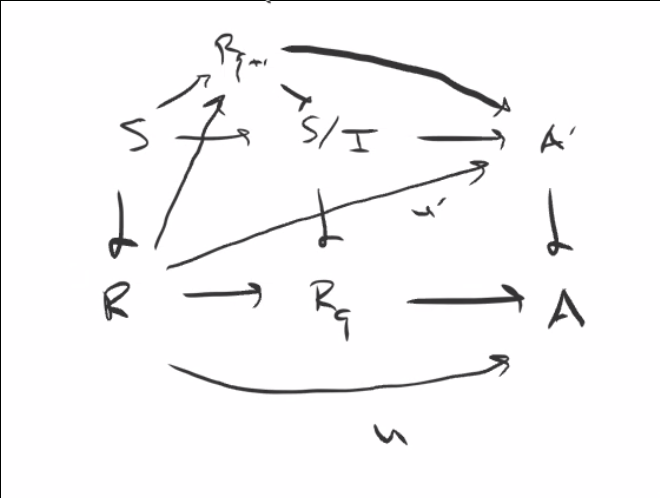
\includegraphics{figures/image_2020-04-07-13-17-11.png}

\todo[inline]{Image to diagram}

where the diagonal map \(u'\) gives us the desired lift, and thus

\begin{center}
\begin{tikzcd}
R \ar[r] \ar[rr, bend left] & R_{q+1} \ar[r] & A'
\end{tikzcd}
\end{center}

exists. This concludes showing miniversality.

\hypertarget{part-of-proof}{%
\subsection{Part of Proof}\label{part-of-proof}}

To finish, we want to show that H4 implies that the map on sections
\(h_R \xrightarrow{\xi} F\) is bijective.

\begin{center}
\begin{tikzcd}
&
&
& h_R 
  \ar[d, "\xi"]
\\
& h_A 
  \ar[rr, bend right, "\eta"] 
  \ar[rru, bend left, "u"] 
& h_{A'} 
  \ar[r, "\eta'"] 
  \ar[ru, "\exists ! u'"] 
& F
\end{tikzcd}
\end{center}

where the map \(\xi\) is ``formal etale'', which will necessarily imply
that it's a bijection over all artinian rings. So we just need to show
formal étaleness. We have a diagram

\begin{center}
\begin{tikzcd}
t_R {\circlearrowleft}u'\in h_R(A') \ar[r] \ar[d] & u\in h_R(A) \ar[d] \\
t_F {\circlearrowleft}\eta' \in h_R(A') \ar[r] & \eta \in h_R(A)
\end{tikzcd}
\end{center}

where \(u'\) exists by smoothness.

Assume that are two \(u', u''\), then \(u' = u'' + \theta\) and
\(\operatorname{im}(u') = \operatorname{im}(u'') + \theta \implies \theta = 0\)
and thus \(u' = u''\).

\hypertarget{revisiting-goals}{%
\subsection{Revisiting Goals}\label{revisiting-goals}}

We originally had two goals:

\begin{enumerate}
\def\labelenumi{\arabic{enumi}.}
\item
  Given a representable moduli functor (such as the Hilbert functor), we
  wanted to understand the local structure by analyzing the deformation
  functor at a given point.
\item
  We want to use representability of the deformation functors to get
  global representability of the original functor.
\end{enumerate}

\begin{question}

What can we now deduce about the local structure of functors using their
deformation theory?

\end{question}

\begin{fact}[1]

Any two hulls \(h_R \to F\) are isomorphic but not canonically. We can
lift maps at every finite level and induct up, which is an isomorphism
on tangent spaces and thus an isomorphism. The sketch: use smoothness to
get the map, and the tangent space condition will imply the full
isomorphism.

\end{fact}

\begin{fact}[3]

Suppose that \(F\) has an obstruction theory (not necessarily strong).
This implies there exists a hull \(h_R \xrightarrow{\xi }F\). The
obstruction theory of \(F\) \emph{gives} an obstruction theory of
\(h_R\): given \(A' \to A\) a small thickening, we need a functorial
assignment
\begin{align*}
t_R = \mathrm{def} {\circlearrowleft}h_R(A') \to h_R(A) \xrightarrow{\mathrm{obs}} \mathrm{obs} \\
\mathrm{def} {\circlearrowleft}F(A') \to F(A) \xrightarrow{\mathrm{obs}} \mathrm{obs}
\end{align*}
where there are vertical maps with equality on the edges.

\begin{figure}
\centering
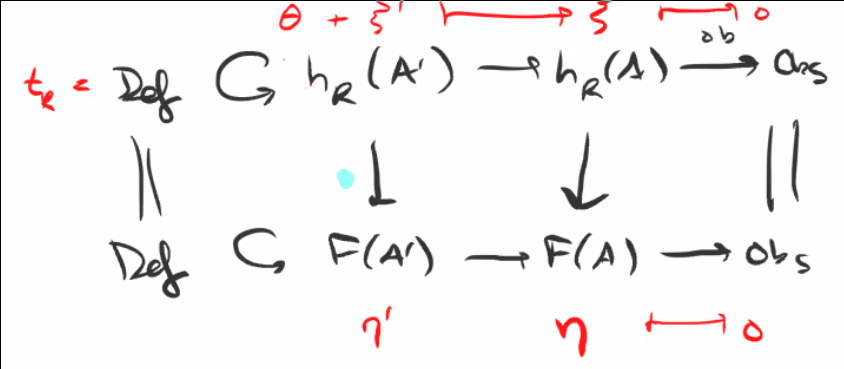
\includegraphics{figures/image_2020-04-07-13-35-00.png}
\caption{Vertical maps}
\end{figure}

By formal smoothness, \(\eta'\) lifts to some \(\xi'\), but using the
transitivity of the action of the tangent space can fix this. We already
had an obstruction theory of \(R\), since we can always find a quotient
\begin{align*}
I \to S = k[[t_R^\vee]] \twoheadrightarrow R
\end{align*}
and \(h_K\) has an obstruction theory

\begin{itemize}
\tightlist
\item
  \(\mathrm{def} = t_R = \qty{{\mathfrak{m}}_R/{\mathfrak{m}}_R^2}^\vee\)
\item
  \(\mathrm{obs} = \qty{I/{\mathfrak{m}}_S I}^\vee\)
\end{itemize}

\end{fact}

\begin{fact}[proof can be found in FGA]

Any other obstruction theory \((\mathrm{def}', \mathrm{obs}')\) of
\(h_R\) admits an injection
\(\qty{I/{\mathfrak{m}}_S I}^\vee\hookrightarrow\mathrm{obs}'\).

\end{fact}

Combining these three facts, we conclude the following: If \(F\) has an
obstruction theory \(\mathrm{def}(F), \mathrm{obs}(F)\), then \(F\) has
a miniversal family \(h_R \xrightarrow{\xi }F\) with \(R = S/ I\) a
quotient of the formal power series ring over some ideal, where
\(S = k[[t_F^\vee]]\). It follows that
\(\dim(I/{\mathfrak{m}}_S I) \leq \dim \mathrm{obs}(F)\), and thus the
minimal number of generators of \(I\) (equal to the LHS by Nakayama) is
bounded by the RHS. Thus
\begin{align*}
\dim_k \mathrm{def}(F) \geq \dim R \geq \dim \mathrm{def}(F) - \dim \mathrm{obs}(F)
.\end{align*}

In particular, if
\(\dim(R) = \dim \mathrm{def}(F) - \dim \mathrm{obs}(F)\), then \(R\) is
a complete intersection. If \(\dim(R) = \dim \mathrm{def}(R)\), the
ideal doesn't have any generators, and \(R \cong S\). In particular, if
\(\mathrm{obs}(F) = 0\), then \(R \cong S\) is isomorphic to this power
series ring.

Finally, if \(F\) is the deformation functor for a global representable
functor, then \(R = \widehat{{\mathcal{O}}}_{{\mathfrak{m}}, p}\) is the
completion of this local ring and the same things hold for this
completion. Thus regularity can be checked on the completion. So if you
have a representable functor with an obstruction theory (e.g.~the
Hilbert Scheme) with zero obstruction, then we have smoothness at that
point. If we know something about the dimension at a point relative to
the obstruction, we can deduce information about being a local
intersection. So the deformation tells you the dimension of a minimal
smooth embedding, and the obstruction is the maximal number of equations
needed to cut it out locally.

\begin{remark}

The content here: see Hartshorne's \emph{Deformation Theory}. The
section in FGA is in less generality but has many good examples. See
``Fundamental Algebraic Geometry''. See also representability of the
Picard scheme.

\end{remark}

\hypertarget{thursday-april-9th}{%
\section{Thursday April 9th}\label{thursday-april-9th}}

Let \(F: \operatorname{Art}_{/k} \to {\operatorname{Set}}\) be a
deformation functor with an obstruction theory. Then H1-H3 imply the
existence of a miniversal family, and gives us some control on the hull
\(h_{R} \to F\), namely
\begin{align*}
\dim \mathrm{def}(F) \geq \dim R \geq \dim \mathrm{def}(F) - \dim \mathrm{obs}(F)
.\end{align*}
In particular, if \(\mathrm{obs}(F) = 0\), then
\(R \cong k[[\mathrm{def}(F)^\vee]] = k[[ t_{F}^\vee]]\).

\begin{example}[?]

Let \(M = \operatorname{Hilb}_{{\mathbb{P}}^n_{/k}}^{dt + (1-g)}\) where
\(k=\mkern 1.5mu\overline{\mkern-1.5muk\mkern-1.5mu}\mkern 1.5mu\), and
suppose \([Z] \in M\) is a smooth point. Then
\begin{align*}
\mathrm{def} = \hom_{ {{ {\mathcal{O}}_{x} }{\hbox{-}}\operatorname{mod}} }(I_{Z}, {\mathcal{O}}_{Z}) = \hom_{Z}(I_{Z}/I_{Z}^2, {\mathcal{O}}_{Z}) = H^0(N_{Z/X})
.\end{align*}
the normal bundle \(N_{Z/X} = (I/I^2)^\vee\) of the regular embedding,
and \(\mathrm{obs} = H^1(N_{Z/X})\).

\begin{claim}

If \(H^1({\mathcal{O}}_{Z}(1)) = 0\) (e.g.~if \(d > 2g-2)\) then \(M\)
is smooth.

\end{claim}

\begin{proof}[of claim]

The tangent bundle of \({\mathbb{P}}^n\) sits in the Euler sequence
\begin{align*}
0 \to {\mathcal{O}}\to {\mathcal{O}}(1)^{n+1} \to T_{{\mathbb{P}}^n} \to 0
.\end{align*}

And the normal bundles satisfies
\begin{align*}
0 \to T_{Z} &\to T_{{\mathbb{P}}^n}\mathrel{\Big|}_{Z} \to N_{Z/{\mathbb{P}}^n} \to 0 \\ \\
&\Downarrow \text{ is the dual of }\\ \\
0 \to I/I^2 &\to \Omega \mathrel{\Big|}_{Z} \to \Omega \to 0
.\end{align*}

There is another SES:
\begin{align*}
?????
.\end{align*}

Taking the LES in cohomology yields
\begin{align*}
H^1({\mathcal{O}}_{Z}(1)^{n+1})=0 \to H^1(N_{Z/{\mathbb{P}}^n}) =0 \to 0
\end{align*}
and thus \(M\) is smooth at \([Z]\). We can compute the dimension using
Riemann-Roch:
\begin{align*}
\dim_{[Z]} M 
&= \dim H^0(N_{Z/{\mathbb{P}}^n}) \\
&= \chi(N_{Z/{\mathbb{P}}^n}) \\
&= \deg N + {\operatorname{rank}}N(1-g) \\
&= \deg T_{{\mathbb{P}}^n} \mathrel{\Big|}_Z - \deg T_{Z} + (n-1)(1-g) \\
&= d(n+1) + (2-2g) + (n-1)(1-g)
.\end{align*}

\end{proof}

\end{example}

\begin{remark}

This is one of the key outputs of obstruction theory: being able to
compute these dimensions.

\end{remark}

\begin{example}[?]

Let \(X \subset {\mathbb{P}}^5\) be a smooth cubic hypersurface and let
\(H = \operatorname{Hilb}_{X_{/k}}^{\text{lines} = t+1} \subset \operatorname{Hilb}_{{\mathbb{P}}^5/k}^{t+1} = {\operatorname{Gr}}(1, {\mathbb{P}}^5)\),
the usual Grassmannian.

\begin{claim}

Let \([\ell] \in H\), then the claim is that \(H\) is smooth at
\([\ell]\) of dimension 4.

\end{claim}

\begin{proof}[of claim]

We have

\begin{itemize}
\tightlist
\item
  \(\mathrm{def} = H^0(N_{\ell/X})\)
\item
  \(\mathrm{obs} = H^1(N_{\ell/X})\)
\end{itemize}

We have an exact sequence
\begin{align*}
0 \to N_{\ell/X} \to N_{\ell/{\mathbb{P}}} \to N_{X/{\mathbb{P}}}\mathrel{\Big|}_\ell \to 0 \\
.\end{align*}

There are surjections from \({\mathcal{O}}_\ell(1)^6\) onto the last two
terms.

\begin{claim}[Subclaim]

For \(N = N_{\ell/{\mathbb{P}}}\) or
\(N_{X/{\mathbb{P}}}\mathrel{\Big|}_\ell\), we have \(H^1(N) = 0\) and
\({\mathcal{O}}(1)^6 \twoheadrightarrow N\) is surjective on global
sections.

\end{claim}

\begin{proof}[of subclaim]

Because \(\ell\) is a line, \({\mathcal{O}}_\ell(1) = {\mathcal{O}}(1)\)
and \(H^1({\mathcal{O}}_\ell(1)) = 0\) and the previous proof applies,
so \(H^1(N) = 0\).

\end{proof}

We thus have a diagram:

\begin{figure}
\centering
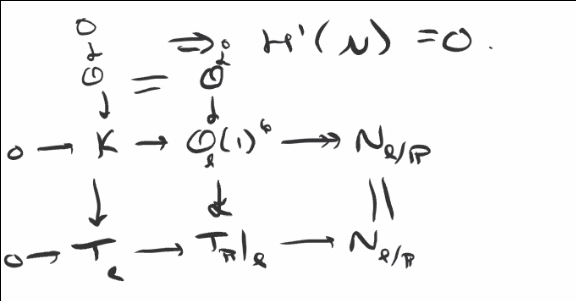
\includegraphics{figures/image_2020-04-09-12-51-51.png}
\caption{Image}
\end{figure}

In particular, \(T_\ell = {\mathcal{O}}(2)\), and the LES for
\(0 \to {\mathcal{O}}\to K \to T_\ell\) shows \(H^1(K) = 0\). Looking at
the horizontal SES
\(0 \to K \to {\mathcal{O}}_\ell(1)^6 \twoheadrightarrow N_{\ell/{\mathbb{P}}}\)
yields the surjection claim. We have

\begin{figure}
\centering
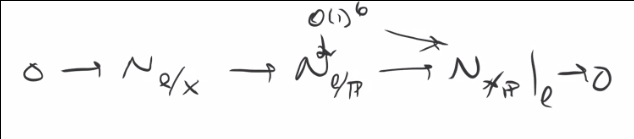
\includegraphics{figures/a.png}
\caption{Diagram}
\end{figure}

and taking the LES in cohomology yields

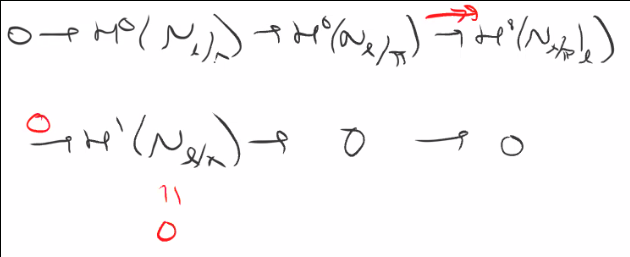
\includegraphics{figures/image_2020-04-09-12-55-01.png}\\

Therefore \(H\) is smooth at \(\ell\) and
\begin{align*}
\dim_\ell H
&= \chi(N_{\ell/X}) \\
&= \deg T_{X} - \deg T_\ell + 3 \\
&= \deg T_{\mathbb{P}}- \deg N_{X/{\mathbb{P}}} - \deg T_\ell + 3 \\
&= 6 - 3 - 2 + 3 = 4
.\end{align*}

\end{proof}

\end{example}

\begin{remark}

It turns out that the Hilbert scheme of lines on a cubic has some
geometry: the Hilbert scheme of two points on a K3 surface.

\end{remark}

\hypertarget{abstract-deformations-revisited}{%
\subsection{Abstract Deformations
Revisited}\label{abstract-deformations-revisited}}

Take \(X_{0} / k\) some scheme and consider the deformation functor
\(F(A)\) taking \(A\) to \(X/A\) flat with an embedding
\(\iota: X_{0} \hookrightarrow X\) with \(\iota \otimes k\) an
isomorphism. Start with H1, the gluing axiom (regarding small
thickenings \(A' \to A\) and a thickening \(A'' \to A\)). Suppose
\begin{align*}
X_{0} \hookrightarrow X' \in F(A') \to F(A)
.\end{align*}
which restricts to \(X_{0} \hookrightarrow X\). Then in \(F(A)\), we
have \(X_{0} \hookrightarrow X' \otimes_{A'} A\), and we obtain a
commutative diagram where \(X' \otimes A \hookrightarrow X'\) is a
closed immersion:

\begin{figure}
\centering
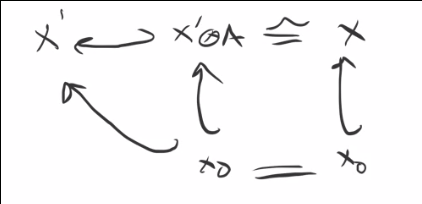
\includegraphics[width=3.64583in,height=\textheight]{figures/abcdefg.png}
\caption{???}
\end{figure}

The restriction \(X' \to X\) means that there exists a diagram

\begin{center}
\begin{tikzcd}
X' 
&  
& X
  \ar[ll, dotted, "\exists"] 
\\
& 
X
  \ar[ur, hook] 
  \ar[ul, hook]
\end{tikzcd}
\end{center}

Note that this is not necessarily unique. We have

\begin{figure}
\centering
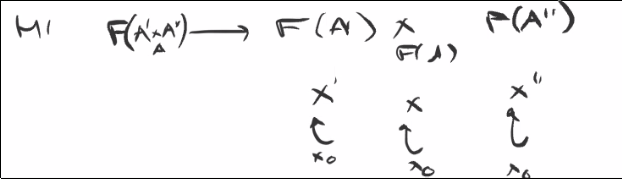
\includegraphics[width=3.64583in,height=\textheight]{figures/image_2020-04-09-13-06-40.png}
\caption{Diagram?}
\end{figure}

This means that we can find embeddings such that

\begin{center}
\begin{tikzcd}
X'' & \ar[l, "\exists", hook] X \ar[r, "\exists", hook] & X' \\
& X_{0} \ar[ul, hook] \ar[u, hook] \ar[ur, hook]
\end{tikzcd}
\end{center}

\begin{figure}
\centering
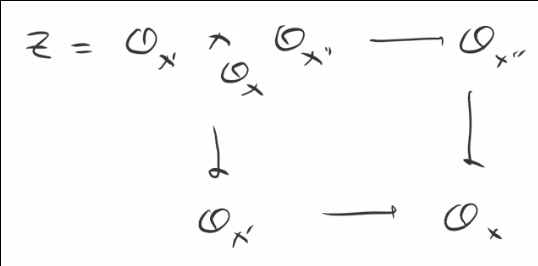
\includegraphics[width=3.64583in,height=\textheight]{figures/image_2020-04-09-13-08-19.png}
\caption{Diagram}
\end{figure}

And thus if we have

\begin{figure}
\centering
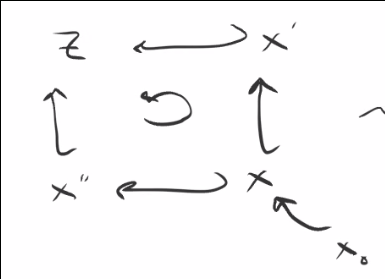
\includegraphics[width=3.64583in,height=\textheight]{figures/image_2020-04-09-13-08-42.png}
\caption{Diagram}
\end{figure}

then \(X_{0} \hookrightarrow Z\) is \textbf{a} required lift (again not
unique).

\begin{question}

When is such a lift unique?

\end{question}

Suppose \(X_{0} \hookrightarrow W\) is another lift, then it restricts
to both \(X, X'\) and we can fill in the following diagrams:

\begin{figure}
\centering
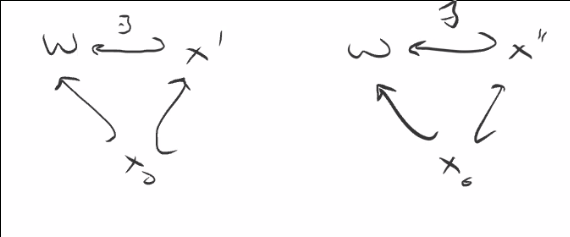
\includegraphics[width=3.64583in,height=\textheight]{figures/image_2020-04-09-13-10-44.png}
\caption{Diagram}
\end{figure}

Using the universal property of \(Z\), which is the coproduct of this
diagram:

\begin{figure}
\centering
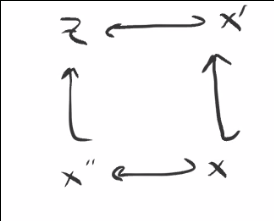
\includegraphics[width=3.64583in,height=\textheight]{figures/image_2020-04-09-13-11-13.png}
\caption{Diagram}
\end{figure}

However, there may be no such way to fill in the following diagram:

\begin{figure}
\centering
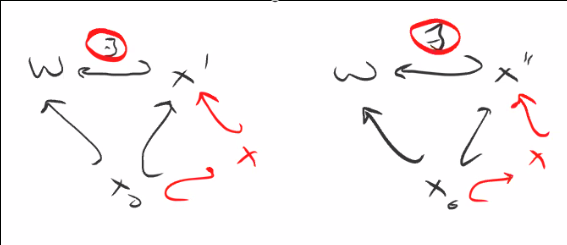
\includegraphics[width=3.64583in,height=\textheight]{figures/image_2020-04-09-13-11-58.png}
\caption{Diagram}
\end{figure}

But if there exists a map making this diagram commute:

\begin{figure}
\centering
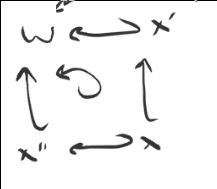
\includegraphics[width=3.64583in,height=\textheight]{figures/image_2020-04-09-13-12-25.png}
\caption{Diagram}
\end{figure}

Then there is a map \(Z\to W\) which is flat after tensoring with \(k\),
which is thus an isomorphism.\footnote{Recall that by Nakayama, a
  nonzero module tensor \(k\) can not be zero.}

\begin{remark}

Thus the lift is unique if

\begin{itemize}
\item
  \(X = X_{0}\), then the following diagrams commute by taking the
  identity and the embedding you have. Note that in particular, this
  implies H2.

  \begin{figure}
  \centering
  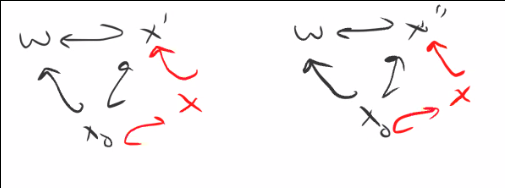
\includegraphics[width=3.64583in,height=\textheight]{figures/image_2020-04-09-13-15-09.png}
  \caption{Diagram}
  \end{figure}
\item
  Generally, these diagrams can be completed (and thus the gluing maps
  are bijective) if the map
  \begin{align*}
  \operatorname{Aut}(X_{0}\hookrightarrow X') \to \operatorname{Aut}(X_{0} \hookrightarrow X)
  .\end{align*}
  of automorphisms of \(X'\) commuting with \(X_{0} \hookrightarrow X\)
  is surjective.
\end{itemize}

\end{remark}

So in this situation, there is only \emph{one} way to fill in this
diagram up to isomorphism:

\begin{figure}
\centering
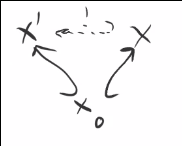
\includegraphics[width=3.64583in,height=\textheight]{figures/image_2020-04-09-13-18-59.png}
\caption{Diagram}
\end{figure}

If we had two ways of filling it in, we obtain bridging maps:

\begin{figure}
\centering
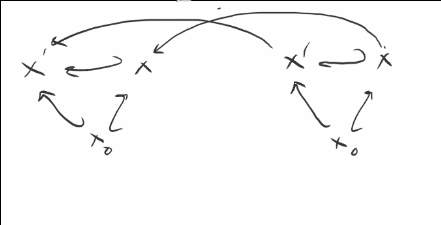
\includegraphics[width=3.64583in,height=\textheight]{figures/image_2020-04-09-13-20-07.png}
\caption{Diagram}
\end{figure}

\begin{lemma}[?]

If \(H^0(X_{0}, T_{X_{0}}) = 0\) (where the tangent bundle always makes
sense as the dual of the sheaf of Kahler differentials) which we can
identify as derivations
\(D_{{\mathcal{O}}_{k}}({\mathcal{O}}_{X_{0}}, {\mathcal{O}}_{X_{0}})\),
then the gluing map is bijective.

\end{lemma}

\begin{proof}[?]

The claim is that \(\operatorname{Aut}(X_{0} \hookrightarrow X) = 1\)
are always trivial. This would imply that all random choices lead to
triangles that commute. Proceeding by induction, for the base case
\(\operatorname{Aut}(X_{0} \hookrightarrow X_{0}) = 1\) trivially.
Assume \(X_{0} \hookrightarrow X_{i}\) lifts
\(X_{0} \hookrightarrow X\), then there's an exact sequence
\begin{align*}
0 
\to 
\operatorname{Der}_{k}({\mathcal{O}}_{X_{0}}, {\mathcal{O}}_{X_{0}}) 
\to  
{\operatorname{Aut}}(X_{0} \hookrightarrow X_0') 
\to 
{\operatorname{Aut}}(X_{0} \hookrightarrow X)
.\end{align*}

\end{proof}

Thus \(F\) always satisfies H1 and H2, and \(H^0(T_{X_{0}}) = 0\) (so no
``infinitesimal automorphism'') implies H4. Recall that the dimension of
deformations of \(F\) over \(k[\varepsilon]\) is finite,
i.e.~\(\dim t_{F} < \infty\) This is where some assumptions are needed.

If \(X_{/K}\) is either

\begin{itemize}
\tightlist
\item
  Projective, or
\item
  Affine with isolated singularities,
\end{itemize}

this is enough to imply H3. Thus by Schlessinger, under these conditions
\(F\) has a miniversal family.

Moreover, if \(H^0(T_{X_{0}}) = 0\) then \(F\) is pro-representable.

\begin{example}[?]

If \(X_{0}\) is a smooth projective genus \(g\geq 2\) curve, then

\begin{itemize}
\tightlist
\item
  Obstruction theory gives the existence of a miniversal family
\item
  We have \(\mathrm{obs} = H^2(T_{X_{0}}) = 0\), and thus the base of
  the miniversal family is smooth of dimension
  \(\mathrm{def}(F) \dim H^1(T_{X_{0}})\),
\item
  \(H^0(T_{X_{0}}) = 0\) and \(\deg T_{X_{0}} = 2-2g < 0\), which
  implies that the miniversal family is universal.
\end{itemize}

We can conclude
\begin{align*}
\dim H^1(T_{X_{0}}) = -\chi(T_{X_{0}}) =  -\deg T_{X_{0}} + g-1 =  3(g-1)
.\end{align*}

\end{example}

\begin{remark}

Note that the global deformation functor is not representable by a
scheme, and instead requires a stack. However, the same fact shows
smoothness in that setting.

\end{remark}

\hypertarget{hypersurface-singularities}{%
\subsection{Hypersurface
Singularities}\label{hypersurface-singularities}}

Consider \(X(f) \subset {\mathbb{A}}^n\), and for simplicity,
\((f=0) \subset {\mathbb{A}}^2\), and let

\begin{itemize}
\item
  \(S = {\mathbb{C}}[x, y]\).
\item
  \(B = {\mathbb{C}}[x, y] / (f)\)
\end{itemize}

\begin{question}

What are the deformations over \(A \coloneqq k[\varepsilon]\)?

\end{question}

This means we have a ring \(B'\) flat over \(k\) and tensors to an
isomorphism, so tensoring \(k\to A\to k\) yields the following:

\begin{center}
\begin{tikzcd}
0 
    \ar[r] 
& B 
    \ar[r] 
& B'
     \ar[r] 
& B 
    \ar[r] 
& 0 
\\
0
    \ar[r]
& S 
    \ar[u] 
    \ar[r] 
& S[\varepsilon] 
    \ar[u, "\exists", twoheadrightarrow] 
    \ar[r] 
& S 
    \ar[r] 
    \ar[u] 
& 0
\\
0 
    \ar[r]
& S \cong I 
    \ar[u] 
    \ar[r] 
& I'= \left\langle{f'}\right\rangle
    \ar[u]
    \ar[r] 
& I = \left\langle{f}\right\rangle 
    \ar[u, "\cong"] 
    \ar[r]
& S
\end{tikzcd}
\end{center}

Thus any such \(B'\) is the quotient of \(S[\varepsilon]\) by an ideal,
and we have \(f' = f + \varepsilon g\).

\begin{question}

When do two \(f'\)s give the same \(B'\)?

\end{question}

We have \(\varepsilon f' = \varepsilon f\), so
\(\varepsilon f \in (f')\) and we can modify \(g\) by any \(cf\) where
\(c\in S\), where only the equivalence class \(g\in S/(f)\) matters. Now
consider \(\operatorname{Aut}(B \hookrightarrow B')\), i.e.~maps of the
form
\begin{align*}
x &\mapsto x + \varepsilon a \\
y &\mapsto y + cb
\end{align*}
for \(a, b\in S\). Under this map,
\begin{align*}
f_0' 
= f + \varepsilon g \mapsto & f(x + \varepsilon a, y + \varepsilon b) + \varepsilon g(x ,y) \\ \\
&\Downarrow \quad\text{implies} \\ \\
f(x, y) &= \varepsilon a {\frac{\partial }{\partial x}\,} f + \varepsilon b {\frac{\partial }{\partial y}\,} f + \varepsilon g(x ,y)
,\end{align*}
so in fact only the class of
\(g\in S/(f, {\partial}_{x} f, {\partial}_{y} f)\). This is the ideal of
the singular locus, and will be Artinian (and thus finite-dimensional)
if the singularities are isolated, which implies H3. We can in fact
exhibit the miniversal family explicitly by taking \(g_{i} \in S\),
yielding a basis of the above quotient. The hull will be given by
setting \(R = {\mathbb{C}}[[t_{1}, \cdots, t_{m} ]]\) and taking the
locus \(V(f + \sum t_{i} g_{i}) \subset {\mathbb{A}}_{R}^2\).

\begin{example}[simple]

For \(f = xy\), then the ideal is \(I = (xy, y, x) = (x, y)\) and
\(C/I\) is 1-dimensional, so the miniversal family is given by
\(V(xy + t) \subset {\mathbb{C}}[[t_{1}]][x, y]\). The greater
generality is needed because there are deformation functors with a hull
but no universal families.

\end{example}

\hypertarget{tuesday-april-14th}{%
\section{Tuesday April 14th}\label{tuesday-april-14th}}

Recall that we are looking at \((X_{0})_{/k}\) and
\(F: \operatorname{Art}_{/k} \to {\operatorname{Set}}\) where \(A\) is
sent to \(X_{/A}\) flat with \(i: X_{0} \hookrightarrow X\) where
\(i\otimes k\) is an isomorphism. The second condition is equivalent to
a cartesian diagram

\begin{center}
\begin{tikzcd}
  X_{0} 
  \ar[r, hook]
  \ar[d] 
  \arrow[dr, phantom, "\scalebox{1.5}{$\ulcorner$}" , very near start, color=black]
& X 
  \ar[d] 
\\
  \operatorname{Spec}k 
  \ar[r, hook] 
& \operatorname{Spec}A
\end{tikzcd}
\end{center}

We showed we always have H1 and H2, and H3 if \(X_{0}/k\) is projective
or \(X_{0}\) is affine with isolated singularities. In this situation we
have a miniversal family. This occurs iff for \(A' \to A\) a small
thickening and \((X_{0} \hookrightarrow X) \in F(A)\), we have a
surjection
\begin{align*}
{\operatorname{Aut}}_{A'}(X_{0} \hookrightarrow X') \twoheadrightarrow{\operatorname{Aut}}_{A}(X_{0} \hookrightarrow X)
.\end{align*}

where the RHS are automorphisms of \(X_{/A}\), i.e.~those which commute
with the identity on \(A\) and \(X_{0}\). We had a naive functor
\(F_{n}\) where we don't include the inclusion
\(X_{0} \hookrightarrow X\). When \(F\) has a hull then the naive
functor has a versal family, since there is a forgetful map that is
formally smooth. If it's the case that for all \(A' \to A\) small and
\(F_{\text{n}} \to F_{n}(A)\) we have
\({\operatorname{Aut}}_{A'}(X') \twoheadrightarrow{\operatorname{Aut}}_{A} (X)\),
then \(F = F_{n}\) and both are pro-representable. The forgetful map is
smooth because given \(X_{/A}\) in \(F_{n}(A)\), we have some inclusion
\(X_{0} \hookrightarrow X\), so one gives surjectivity. Using the
surjectivity on automorphisms, we get

\begin{center}
\begin{tikzcd}
X_{0}\ar[rd, hook] \ar[rr, hook] & & X\ar[ld, dotted] \\
& X & 
\end{tikzcd}
\end{center}

Deformation theory is better at answering when the following diagrams
exist:

\begin{center}
\begin{tikzcd}
X 
  \ar[r, dotted, hook, "\exists?"] 
  \ar[d]
  \arrow[dr, phantom, "\scalebox{1.5}{$\ulcorner$}" , shift right=0.4em, very near start, color=black]
& 
X'
  \ar[d, dotted, "\exists?"] 
\\
\operatorname{Spec}A
  \ar[r]
& 
\operatorname{Spec}A' 
\end{tikzcd}
\end{center}

i.e., the existence of an extension of \(X\) to \(A'\). This is
different than understanding diagrams of the following type, where we're
considering isomorphism classes of the squares, and deformation theory
helps understand the blue one:

\begin{center}
\begin{tikzpicture}
[
    greenbox/.style={
        draw=green, fill=green!3,  thick, rounded corners, rectangle
    },
    redbox/.style={
        draw=red, fill=red!3,  thick, rounded corners, rectangle
    },
]

\node[
    greenbox,   
    minimum height=0.9cm,
    minimum width=1.2cm 
] 
at (-0.1, 1.3) {};

\node[
    redbox, 
    minimum height=0.9cm,
    minimum width=1.2cm 
] 
at (2.35, 1.3) {};

\node[
    greenbox, 
    minimum height=2.4cm,
    minimum width=8.2cm 
] 
at (0, -0.5) {};

\node[
    draw=red,  thick, rectangle,
    minimum height=0.8cm,
    minimum width=1.2cm 
] 
at (-1.2, -0.6) {};

\node[
    draw=blue,  thick, rectangle, dotted,
    minimum height=0.8cm,
    minimum width=1.2cm 
] 
at (1.2, -0.6) {};

\node at (0, 0) {%
\begin{tikzcd}
& F(A')
    \ar[r]
& F(A)
\\
X_0
    \ar[r, hook]
    \ar[d]
& X
    \ar[r, hook]
    \ar[d]
& X'
    \ar[d]
\\
\operatorname{Spec}k
    \ar[r]
& \operatorname{Spec}A
    \ar[r]
& \operatorname{Spec}A'
\end{tikzcd}
};

\end{tikzpicture}
\end{center}

\begin{example}[Hypersurface Singularities]

Take \(S = k[x, y]\) and \(B = S/(f)\), then deformations of
\(\operatorname{Spec}B\) to ? Given \(k \to k[\varepsilon] \to k\) we
can tensor\footnote{For flat maps, tensoring up to an isomorphism
  implies isomorphism.} to obtain

\begin{center}
\begin{tikzcd}
    {0} & {B} & {B'} & {B} & {0} \\
    {0} & {S} & {S[\varepsilon]} & {S} & {0} \\
    {0} & {I} & {I'} & {I} & {0} \\
    && {\tiny \left\langle{f'}\right\rangle} & {\tiny \left\langle{f}\right\rangle}
    \arrow[from=3-1, to=3-2]
    \arrow[from=3-2, to=3-3]
    \arrow[from=3-3, to=3-4]
    \arrow[from=3-4, to=3-5]
    \arrow[from=1-1, to=1-2]
    \arrow[from=1-2, to=1-3]
    \arrow[from=1-3, to=1-4]
    \arrow[from=1-4, to=1-5]
    \arrow[from=2-1, to=2-2]
    \arrow[from=2-2, to=2-3]
    \arrow[from=2-3, to=2-4]
    \arrow[from=2-4, to=2-5]
    \arrow[from=3-2, to=2-2]
    \arrow["{\pi}", from=2-2, to=1-2]
    \arrow[from=3-3, to=2-3]
    \arrow["{\pi'}", from=2-3, to=1-3]
    \arrow[from=3-4, to=2-4]
    \arrow["{\pi}", from=2-4, to=1-4]
    \arrow["{\subseteq}" description, from=4-3, to=3-3, no head]
    \arrow["{\subseteq}" description, from=4-4, to=3-4, no head]
\end{tikzcd}
\end{center}

\begin{quote}
\href{https://q.uiver.app/?q=WzAsMTcsWzAsMCwiMCJdLFsxLDAsIkIiXSxbMiwwLCJCJyJdLFszLDAsIkIiXSxbNCwwLCIwIl0sWzAsMSwiMCJdLFsxLDEsIlMiXSxbMiwxLCJTW1xcZXBzXSJdLFs0LDEsIjAiXSxbNCwyLCIwIl0sWzAsMiwiMCJdLFszLDEsIlMiXSxbMSwyLCJJIl0sWzMsMiwiSSJdLFsyLDIsIkknIl0sWzIsMywiXFxnZW5ze2YnfSJdLFszLDMsIlxcZ2Vuc3tmfSJdLFsxMCwxMl0sWzEyLDE0XSxbMTQsMTNdLFsxMyw5XSxbMCwxXSxbMSwyXSxbMiwzXSxbMyw0XSxbNSw2XSxbNiw3XSxbNywxMV0sWzExLDhdLFsxMiw2XSxbNiwxLCJcXHBpIl0sWzE0LDddLFs3LDIsIlxccGknIl0sWzEzLDExXSxbMTEsMywiXFxwaSJdLFsxNSwxNCwiXFxzdWJzZXRlcSIsMSx7InN0eWxlIjp7ImhlYWQiOnsibmFtZSI6Im5vbmUifX19XSxbMTYsMTMsIlxcc3Vic2V0ZXEiLDEseyJzdHlsZSI6eyJoZWFkIjp7Im5hbWUiOiJub25lIn19fV1d}{Link
to diagram.}
\end{quote}

\begin{figure}
\centering
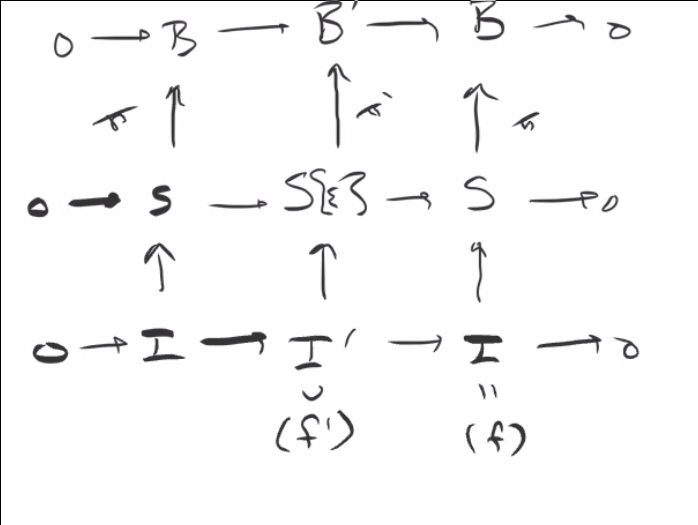
\includegraphics[width=3.64583in,height=\textheight]{figures/image_2020-04-14-12-55-58.png}
\caption{Diagram}
\end{figure}

We want to understand \(F(k[\varepsilon])\). We know
\(f' = f + \varepsilon g\) for some \(g\in S\).

\begin{observation}

\envlist

\begin{enumerate}
\def\labelenumi{\arabic{enumi}.}
\tightlist
\item
  \(g\in B\) and \(f'' = f + \varepsilon(g + cf)\) generates the same
  ideal.
\item
  We're free to reparameterize, i.e.~\(x \mapsto x + \varepsilon a\) and
  \(y \mapsto y + \varepsilon b\) and thus\\
  \begin{align*}
  g \mapsto g + a f_{x} + b f_{y}
  \end{align*}
  , i.e.~the partial derivatives.
\end{enumerate}

\end{observation}

Thus isomorphism classes of \(B'\) in deformations \(B' \to B\) only
depend on the isomorphism classes \(g\in B/(f_{x}, f_{y}) B\). When the
singularities are isolated, this quotient is finite-dimensional as a
\(k{\hbox{-}}\)vector space.

\end{example}

\begin{example}[?]

\(F(k[\varepsilon]) = B/(f_{x}, f_{y})B\). Thus H3 holds and there is a
miniversal family \(h_{R} \to F\). We can describe it explicitly: take
\(g_{i} \in S\), yielding a \(k{\hbox{-}}\)basis in
\(S/(f, f_{x}, f_{y})\). Then
\begin{align*}
V(f + \sum t_{i} g_{i}) \subset \operatorname{Spec}k[[t_{1}, \cdots, t_{n}]][x, y]
.\end{align*}
Set \(R = k[[t_{1}, \cdots, t_{n}]]\), then this lands in
\({\mathbb{A}}_{R}^2\).

\end{example}

\begin{example}[?]

The nodal curve \(y^2 = x^3\), take .
\begin{align*}
S/(y^2-x^3, 2y, -3x^2) = S/(y, x^2)
.\end{align*}
So take \(g_{1} = 1, g_{2} = x\), then the miniversal family is .
\begin{align*}
V(y^2 - x^3 + t + t_{2} x) \subset {\mathbb{A}}^2_{k[[t_{1}, t_{2}]]}
.\end{align*}
This gives all ways of smoothing the node.

\end{example}

\begin{remark}

Note that none of these are pro-representable.

\end{remark}

Given \(X\) and \(A\), we obtain a miniversal family over the formal
spectrum \(\mathrm{Spf}(R) = (R, \xi)\) and a unique map:

\begin{figure}
\centering
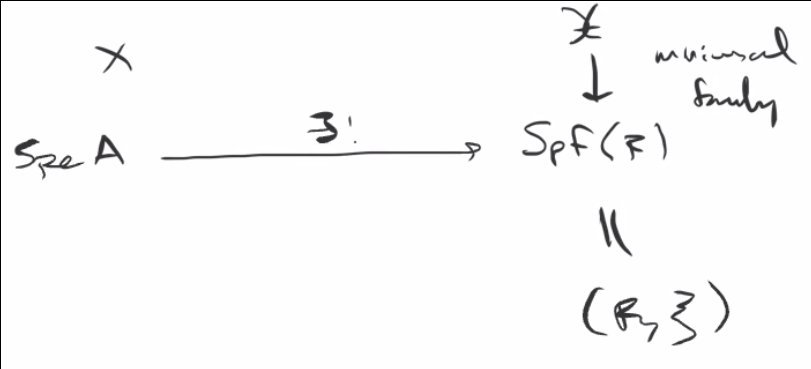
\includegraphics[width=3.64583in,height=\textheight]{figures/image_2020-04-14-13-10-21.png}
\caption{Diagram}
\end{figure}

We can take two deformations over \(A = k[\xi]/ S^n\):

\begin{itemize}
\tightlist
\item
  \(X_{1} = V(x + y)\)??
\item
  \(X_{2} = V(x + uy)\)??
\end{itemize}

As deformations over \(A\), \(X_{1} \cong X_{2}\) where we send ,
\begin{align*}
s&\mapsto s, \\
y&\mapsto y, \\
x&\mapsto ux
.\end{align*}
since
\begin{align*}
(xy + us) = (uxy + us) = (u(xy + s)) = (xy + s)
.\end{align*}
But we have two different classifying maps, which do commute up to an
automorphism of \(A\), but are not equal. Since they pullback to
different elements (?), \(F\) can not be pro-representable.

\begin{figure}
\centering
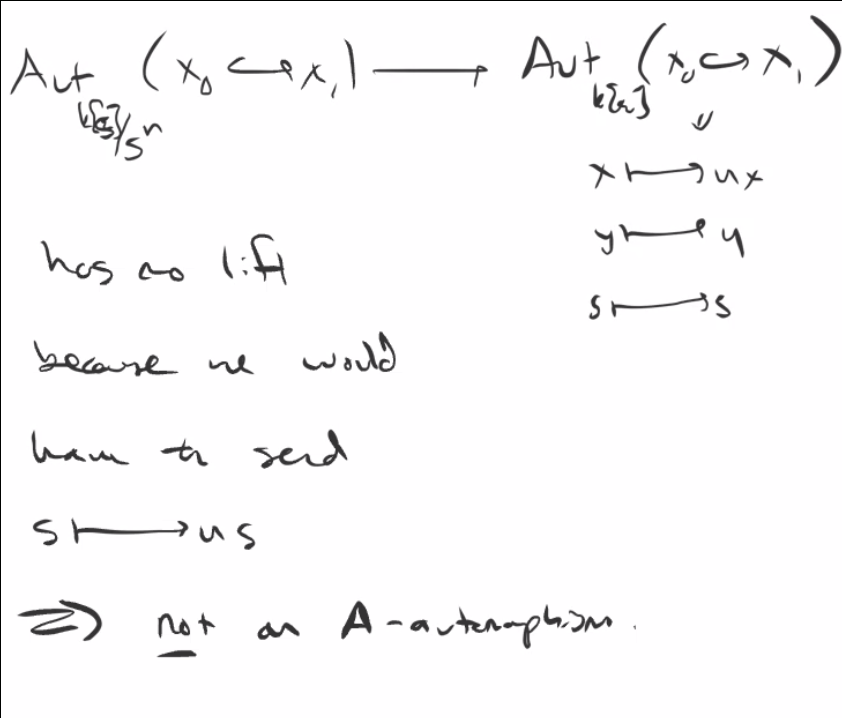
\includegraphics[width=3.64583in,height=\textheight]{figures/image_2020-04-14-13-20-05.png}
\caption{Diagram}
\end{figure}

So reparameterization in \(A\) yield different objects in \(F(A)\). In
other words, \({\mathcal{X}}\to \mathrm{Spf}(R)\) has automorphisms
inducing reparameterizations of \(R\). This indicates why we need maps
restricting to the identity.

\hypertarget{the-cotangent-complex}{%
\subsection{The Cotangent Complex}\label{the-cotangent-complex}}

For \(X \xrightarrow{f} Y\), we have
\(L_{X/Y} \in D {\mathrm{QCoh}}(X)\), the derived category of
quasicoherent sheaves on \(X\). This answers the extension question:

\begin{answer}

For any square-zero thickening \(Y \hookrightarrow Y'\) (a closed
immersion) with ideal \(I\) yields an
\({\mathcal{O}}_{Y}{\hbox{-}}\)module.

\begin{enumerate}
\def\labelenumi{\arabic{enumi}.}
\tightlist
\item
  An extension exists iff
  \(0 = \mathrm{obs} \in \operatorname{Ext}^2(L_{X/Y}, f^* I)\)
\item
  If so, the set of ways to do so is a torsor over this ext group.
\item
  The automorphisms of the completion are given by
  \(\hom(L_{X/Y}, f^* I)\).
\end{enumerate}

\end{answer}

\begin{remark}

Some special cases: \(X \to Y\) smooth yields
\(L_{X/Y} = \Omega_{X/Y}[0]\) concentrated in degree zero.

\end{remark}

\begin{example}[?]

\(Y = \operatorname{Spec}k\) and
\(Y' = \operatorname{Spec}k[\varepsilon]\) yields
\begin{align*}
\mathrm{obs} \in \operatorname{Ext}_{x}^2(\Omega_{X/Y}, {\mathcal{O}}_{x})= H^2(T_{X_{/k}})
.\end{align*}

For \(X\hookrightarrow Y\) is a regular embedding (closed immersion and
locally a regular sequence) \(L_{X/Y} = \qty{I/I^2}[1]\), the conormal
bundle.

\begin{figure}
\centering
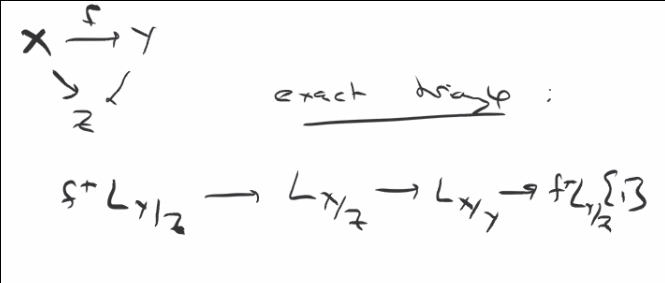
\includegraphics[width=3.64583in,height=\textheight]{figures/image_2020-04-14-13-32-13.png}
\caption{Diagram}
\end{figure}

\end{example}

\begin{example}[?]

For \(Y\) smooth, \(X \hookrightarrow Y\) a regular embedding,
\(L_{X_{/k}} = \Omega_{X_{/k}}\) with
\(\mathrm{obs}/\mathrm{def} = \operatorname{Ext}^{2/1}(\Omega_{x}, {\mathcal{O}})\)
and the infinitesimal automorphisms are the homs.

\end{example}

\begin{example}[?]

For \(Y = \operatorname{Spec}k[x, y] = {\mathbb{A}}^2\) and
\(X = \operatorname{Spec}B = V(f) \subset {\mathbb{A}}^2\) we get
\begin{align*}
0 \to I/I^2 \to \Omega_{X_{/k}} \otimes B &\to \Omega_?{X_{/k}} \to 0 \\ \\
& \Downarrow \quad \text{equals} \\ \\
0 \to B \xrightarrow{1 \mapsto (f_{x}, f_{y})} &B^2 \to \Omega_{B_{/k}} = L_{X_{/k}} \to 0
.\end{align*}

Taking \(\hom({\,\cdot\,}, B)\) yields

\begin{center}
\begin{tikzcd}
0 
  \ar[r]
& \hom(\Omega, B) 
  \ar[r]
& B^2 
  \ar[lld, "{(f_{x}, f_{y})^t}"]
\\
  \operatorname{Ext}^1(\Omega, B) 
  \ar[r]
& 0 
  \ar[r] 
& 0 
  \ar[lld]
\\
  \operatorname{Ext}^2(\Omega, B) 
  \ar[r] 
& 0 
  \ar[r] 
& 0
\end{tikzcd}
\end{center}

So ,
\begin{align*}
\mathrm{obs} &= 0 \\ 
\mathrm{def} &= B/(f_{x}, f_{y})B \\
\operatorname{Aut}&\neq 0
.\end{align*}
and

\end{example}

\begin{remark}

We have the following obstruction theories:

\begin{itemize}
\item
  For abstract deformations, we have
  \begin{align*}
  X_{0} {}_{/k} \text{ smooth } \implies 
  \operatorname{Aut}/\mathrm{def}/\mathrm{obs} = H^{0/1/2}(T_{X_{0}})
  .\end{align*}
\item
  For embedded deformations, \(Y_{0}/k\) smooth,
  \(X_{0} \hookrightarrow Y_{0}\) regular, we have
  \begin{align*}
  \operatorname{Aut}/\mathrm{def}/\mathrm{obs} = 0, H^{0/1}(N_{X_{0}/Y_{0}})
  .\end{align*}

  \begin{quote}
  As an exercise, interpret this in terms of \(L_{X_{0}/Y_{0}}\).
  \end{quote}
\item
  For maps \(X_{0} \xrightarrow{f_{0}} Y_{0}\), i.e.~maps
  \begin{align*}
  X_{0} \times k[\varepsilon] \xrightarrow{f} Y_{0} \times k[\varepsilon]
  .\end{align*}
  we consider the graph \(\Gamma(f_{0}) \subset X_{0} \times Y_{0}\).
\end{itemize}

\begin{figure}
\centering
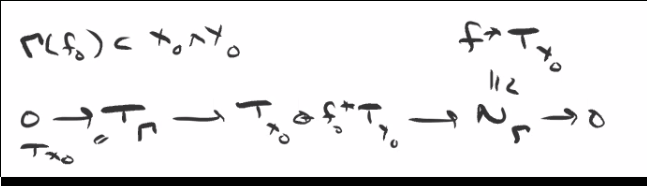
\includegraphics[width=3.64583in,height=\textheight]{figures/image_2020-04-14-13-43-40.png}
\caption{Diagram}
\end{figure}

Since all of these structures are special cases of the cotangent
complex, they place nicely together in the following sense: Given
\(X \hookrightarrow_{i} Y\) we have
\begin{align*}
0 \to T_{X} \to i^* T_{Y} \to N_{X/Y} \to 0
.\end{align*}

Yielding a LES
\begin{align*}
0 &\to H^0(T_{X}) \to H^0(i^* T_{Y}) \to H^0(N_{X/Y}) \\
&\to H^1(T_{X}) \to H^1(i^* T_{Y}) \to H^1(N_{X/Y}) \\
&\to H^2(T_{X}) 
.\end{align*}

\begin{figure}
\centering
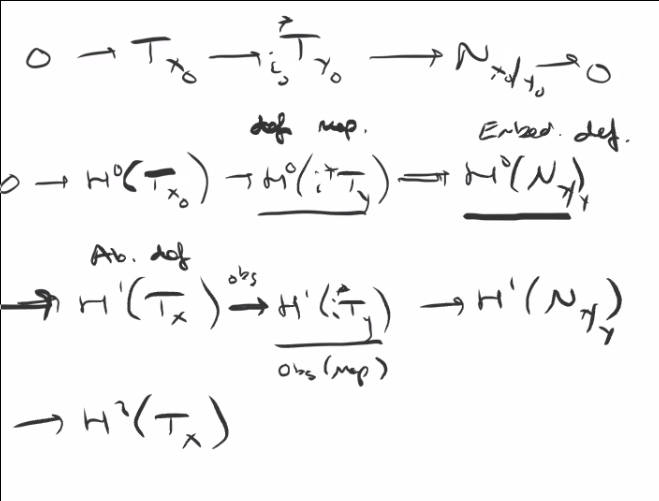
\includegraphics[width=3.64583in,height=\textheight]{figures/image_2020-04-14-13-47-05.png}
\caption{Diagram}
\end{figure}

\end{remark}

\begin{exercise}[?]

Consider \(X \subset {\mathbb{P}}^3\) a smooth quartic, and show that
\(\mathrm{def}(X) \cong k^{20}\) but
\(\mathrm{def}_{\text{embedded}} \cong k^{19}\). This is a quartic K3
surface for which deformations don't lift (non-algebraic, don't sit
inside any \({\mathbb{P}}^n\)).

\end{exercise}

\begin{quote}
Next time: Obstruction theory of sheaves, T1 lifting as a way to show
unobstructedness.
\end{quote}

\hypertarget{characterization-of-smoothness-thursday-april-16th}{%
\section{Characterization of Smoothness (Thursday April
16th)}\label{characterization-of-smoothness-thursday-april-16th}}

\begin{quote}
Recap from last time: the cotangent complex answers an extension
problem.
\end{quote}

Given \(X \xrightarrow{f} Y\) and \(Y \hookrightarrow Y'\) a square zero
thickening. When can the pullback diagram be filled in?

\begin{center}
\begin{tikzcd}
  X  
  \ar[r, dotted] 
  \ar[d] \arrow[dr, phantom, "\scalebox{1.5}{\color{black}$\lrcorner$}" , very near start, color=black]
& X' 
  \ar[d, dotted] 
\\
  Y 
  \ar[r] 
& Y'
\end{tikzcd}
\end{center}

\begin{itemize}
\tightlist
\item
  The existence is governed by
  \(\mathrm{obs} \in \operatorname{Ext}^2( L_{X/Y}, f^* I)\)
\item
  The number of extensions by \(\operatorname{Ext}^1( L_{X/Y}, f^* I)\)
\item
  The automorphisms by \(\operatorname{Ext}^0( L_{X/Y}, f^* I)\)
\end{itemize}

Suppose we're considering \(k[\varepsilon] \to k\), where
\(L_{X_{/k}} = \Omega_{X_{/k}}\), and \(H^*(T_{X_{/k}})\) houses the
obstruction theory. For an embedded deformation \(X \hookrightarrow Y\),
we have

\begin{center}
\begin{tikzcd}
X  
  \ar[r, dotted]
& X' 
  \ar[d, dotted] 
\\
Y 
  \ar[r] 
& Y \times_{\operatorname{Spec}k} \operatorname{Spec}k[\varepsilon]
\end{tikzcd}
\end{center}

then \(L_{X/Y} = I/I^2 [1] = N_{X/Y}^\vee[1]\) and
\begin{align*}
\mathrm{obs} \in \operatorname{Ext}^2(N^\vee[1], {\mathcal{O}}) = \operatorname{Ext}^1(N^\vee, {\mathcal{O}}) = H^1(N)
.\end{align*}
and similarly \(\mathrm{def} = H^0(N)\) and \(\operatorname{Aut}= 0\).
For \(X \xrightarrow{f} Y\), we can think of this as an embedded
deformation of \(\Gamma \subset X \times Y\), in which case
\(N^\vee= F^* \Omega_{Y_{/k}}\). Then
\(\mathrm{obs}, \mathrm{def} \in H^{1, 0}(f^* T_{X_{/k}})\) respectively
and \(\operatorname{Aut}= 0\). There is an exact triangle
\begin{align*}
f^* L_{Y_{/k}} \to L_{X_{/k}} \to L_{X/Y} \to f^* L_{Y_{/k}}[1]
.\end{align*}

\hypertarget{t1-lifting}{%
\subsection{T1 Lifting}\label{t1-lifting}}

This will give a criterion for a pro-representable functor to be smooth.
We've seen a condition on \(F\) with obstruction theory for the hull to
be smooth, namely \(\mathrm{obs}(F) = 0\). However, often \(F = h_{R}\)
will have \(R\) smooth with a natural obstruction theory for which
\(\mathrm{obs}(F) \neq 0\).

\begin{example}[?]

For \(X_{/k}\) smooth projective, the picard functor
\({\operatorname{Pic}}_{X_{/k}}\) is smooth because we know it's an
abelian variety. We also know that the natural obstruction space is
\(\mathrm{obs} = H^2({\mathcal{O}}_{X})\), which may be nonzero. We
could also have abstract deformations given by \(H^2(T_{X})\)

Given \(A \in \operatorname{Art}_{/k}\) and \(M\) a finite length
\(A{\hbox{-}}\)module, we can form the ring \(A \oplus M\) where \(M\)
is square zero and \(A\curvearrowright M\) by the module structure. This
yields
\begin{align*}
0 \to M \to A \oplus M \to A \to 0
\end{align*}

The explicit ring structure is given by
\((x, y) \cdot (x, y') = (xx', x'y + xy')\).

\end{example}

\begin{proposition}[Characterization of Smoothness]

Assume \(\operatorname{ch}k =0\) and \(F\) is a pro-representable
deformation functor, so \(F = \hom(R, \cdot)\) where \(R\) is a complete
local \(k{\hbox{-}}\)algebra with \(\dim t_{R} < \infty\).

Then \(R\) is smooth\footnote{I.e. \(R \cong k[[t_{R}^\vee]]\).} over
\(k\) \(\iff\) for all \(A\in \operatorname{Art}_{/k}\) and all
\(M, M' \in A{\hbox{-}}\text{mod}\) finite dimensional with
\(M \twoheadrightarrow M'\), we have

\begin{align*}
F(A\oplus M) \twoheadrightarrow F(A\oplus M')
.\end{align*}

\end{proposition}

\hypertarget{proof-of-proposition-2}{%
\subsubsection{Proof of Proposition}\label{proof-of-proposition-2}}

\begin{observation}

First observe that
\(\ker(F(A\oplus M) \to F(A)) = \ker(\hom(R, A\oplus M) \to \hom(R, A))\),
note that if we have two morphisms

\begin{center}
\begin{tikzcd}
R 
  \ar[r] 
& 
R
  \ar[r, shift left=0.75ex, "g \oplus g"] 
  \ar[r, shift right=0.75ex, "f \oplus g'"'] 
& 
A \oplus M
\end{tikzcd}
\end{center}

denoting these maps \(h, h'\) we have

\begin{enumerate}
\def\labelenumi{\arabic{enumi}.}
\item
  \(g-g' \in \operatorname{Der}_{k}(R, M)\), since
  \begin{align*}
  (h-h')(x, y) 
  &= h(x)h(y) - h'(x) h'(y) \\
  &= (f(x)f(y), f(x)g(y) + f(y)g(x) )  - (f(x)f(y), f(x) g'(y) + f(y) g'(x)) \\
  &= f(x)(g-g')(y) + f(y)(g-g')(x)
  .\end{align*}
\item
  Given \(g: R\to A\oplus M\) and
  \(\theta \in \operatorname{Der}_{k}(R, M)\), then
  \(g + \theta: R \to A\oplus M\).
\end{enumerate}

\end{observation}

We conclude that the fibers are naturally torsors for
\(\operatorname{Der}_{k}(R, M)\) if nonempty. It is in fact a
canonically trivial torsor, since there is a distinguished element in
each fiber. Thus to show the following, it is enough to show surjection
on fibers and trivial extensions go to trivial ones, then
\(\operatorname{Der}_{k}(R, M) \to \operatorname{Der}_{k}(R, M')\) with
\(0\mapsto 0\).

\begin{center}
\begin{tikzcd}
F(A\oplus M) 
  \ar[rr]
  \ar[rd]
& 
& F(A\oplus M') 
  \ar[ld]
\\
& F(A) 
&
\end{tikzcd}
\end{center}

The criterion for \(F\) being surjective is equivalent to
\begin{align*}
\operatorname{Der}_{k}(R, M) &\twoheadrightarrow\operatorname{Der}_{k}(R, M') \\ \\
&\Downarrow \qquad \text{identified as }\\ \\
\hom_{R}(\Omega_{R_{/k}}, M) &\twoheadrightarrow\hom(\Omega_{R_{/k}'}, M')
.\end{align*}

\begin{warnings}

\(\Omega_{R_{/k}}\) is complicated. An example is
\begin{align*}
\Omega_{k[[x]]/k} \otimes k((x)) = \Omega_{k((x))/k}
.\end{align*}
which is an infinite dimensional \(k((x))\) vector space.

\end{warnings}

Here we only need to consider the completions
\(\hom_{R}(\widehat{\Omega}_{R_{/k}}, M) \twoheadrightarrow\hom(\widehat{\Omega}_{R_{/k}'}, M') = k[[x]]~dx\).

\begin{fact}

In characteristic zero, \(R?k\) is smooth iff
\(\widehat{\Omega}_{R_{/k}}\) is free.

\end{fact}

Thus the surjectivity condition is equivalent to checking that
\(\hom(\widehat{\Omega}_{R_{/k}}, {\,\cdot\,})\) is right-exact on
finite length modules. This happens iff \(\widehat{\Omega}\) are
projective iff they are free.

\begin{fact}[from algebra]

Uses an algebra fact: for a complete finitely-generated module \(M\)
over a complete ring, then \(M\) is free if \(M\) projective with
respect to sequences of finite-length modules. Over a local ring,
finitely-generated and projective implies free.

\end{fact}

\begin{remark}

This is powerful -- allows showing deformations of Calabi-Yaus are
unobstructed!

\end{remark}

\begin{definition}[Calabi-Yau]

A smooth projective \(X_{/k}\) is \textbf{Calabi-Yau} iff
\begin{align*}
\omega_{x} \cong {\mathcal{O}}_{x}
,\end{align*}
i.e.~the canonical bundle is trivial.

\end{definition}

\begin{proposition}[?]

\(X_{/k}\) CY with \(H^0(T_{X}) = 0\) (implying that the deformation
functor \(F\) of \(X\) is pro-representable, say by \(R\), and has no
infinitesimal automorphisms) has unobstructed deformations, i.e.~\(R\)
is smooth of dimension \(H^1(T_{X})\).

\end{proposition}

Note that \(H^2(T_{X}) \neq 0\) in general, so this is a finer
criterion.

\begin{example}[?]

Take \(X \subset {\mathbb{P}}^4\) a smooth quintic threefold.

\begin{itemize}
\item
  By adjunction, this is Calabi-Yau since
  \begin{align*}
  \omega_{x} = \omega_{{\mathbb{P}}^4}(5) \mathrel{\Big|}_{X} = {\mathcal{O}}_{x}
  .\end{align*}
\item
  By Lefschetz,
  \begin{align*}
  H^i_\mathrm{sing} ({\mathbb{P}}^4, {\mathbb{C}}) 
  &\xrightarrow{\cong} 
  H^i_{\mathrm{sing}}(X, {\mathbb{C}})
  && \text{except in middle dimension} \\ \\
  &\Downarrow \quad \text{ implies} \\ \\
  H^{3, 1} 
  &= H^{1, 3} = 0
  .\end{align*}
\item
  By Serre duality,
  \begin{align*}
  H^0(T_{x}) &= 0 \cong H^4(\Omega_{x} \otimes\omega_{x}) \\ \\
  &\Downarrow \quad\text{implies} \\ \\
  H^3(\Omega_{x}) &= H^{3, 1} = 0
  .\end{align*}
\end{itemize}

\end{example}

\begin{exercise}[?]

There are nontrivial embedded deformations that yield the same abstract
deformations, write them down for the quintic threefold.

\end{exercise}

\begin{claim}

The abstract moduli space here is given by
\(\operatorname{PGL}(5) \setminus\operatorname{Hilb}\) where
\(\operatorname{Hilb}\) is smooth.

\end{claim}

\hypertarget{proof-that-obstructions-to-deformations-of-calabi-yaus-are-unobstructed}{%
\subsubsection{Proof that obstructions to deformations of Calabi-Yaus
are
unobstructed}\label{proof-that-obstructions-to-deformations-of-calabi-yaus-are-unobstructed}}

We need to show that for any \(M \twoheadrightarrow M'\) that
\begin{align*}
F(A\oplus M) \twoheadrightarrow F(A\oplus M')
.\end{align*}
The fibers of the LHS are extensions from \(A\) to \(A\oplus M\), and
the RHS are extensions of \(X/A\)? By dualizing, we need to show
\(H^1(T_{X/A}\otimes M ) \twoheadrightarrow H^1(T_{X/A} \otimes M')\)
since the LHS is \(\operatorname{Ext}^1(\Omega_{X/A}, M)\). We want the
bottom map here to be surjective:

\begin{center}
\begin{tikzcd}
  X  
  \ar[d]
& X' 
  \ar[d] 
\\
  \operatorname{Spec}A 
  \ar[r, hook] 
& \operatorname{Spec}A \oplus M
\end{tikzcd}
\end{center}

\begin{fact}[Important]

For \(X/A\) a deformation of a CY, \(H^*(T_{X/A})\) is free. This will
finish the proof, since the map is given by
\(H^1(T_{X/A}) \otimes M \twoheadrightarrow H^1(T_{X/A}) \otimes M'\) by
exactness. This uses the fact that there's a spectral sequence
\begin{align*}
\operatorname{Tor}_{q}(H^p(T_{X/A}), M) \implies H^{p+q} (T_{X/A} \otimes M)
\end{align*}
which follows from base change and uses the fact that \(T_{X/A}\) is
flat.

\end{fact}

We'll be looking at \(\operatorname{Tor}_{1}(H^0(T_{X/A}), M)\) which is
zero by freeness. Hodge theory is now used: by Deligne-Illusie, for
\(X\xrightarrow{f} S\) smooth projective, taking pushforwards
\(R^p f_* \Omega^q_{X_{/S}}\) are free (coming from degeneration of
Hodge to de Rham) and commutes with base change.

\begin{remark}

This implies that \(\omega_{X/A} = {\mathcal{O}}_{X}\) is trivial. Using
Deligne-Illusie, since \(\omega\) is trivial on the special fiber,
\(H^0(\omega_{X/A}) = A\) is free of rank 1. We thus have a section
\({\mathcal{O}}_{X} \to \omega_{X/A}\) which is an isomorphism by
flatness, since it's an isomorphism on the special fiber.

\end{remark}

\begin{remark}

By Serre duality,
\(H^1(T_{X/A}) = H^{n-1}(\Omega_{X/A} \otimes\omega_{X/A}) ^\vee= H^{n-1}(\Omega_{X/A})^\vee\),
which is free by Deligne-Illusie. This also holds for
\(H^0(T_{X/A}) = H^n(\Omega_{X/A})^\vee\) is free.

\end{remark}

Thus deformations of Calabi-Yaus are unobstructed.

\hypertarget{remarks}{%
\subsubsection{Remarks}\label{remarks}}

\begin{remark}

In fact we need much less. Take \(A_{n} = k[t] / t^n\), then consider

\begin{center}
\begin{tikzcd}
0
  \ar[r]
& A_n   
  \ar[r]
& A_n[\varepsilon]
  \ar[r]
& A_n \\
0
  \ar[r]
  \ar[u, equal]
& A_n   
  \ar[r]
  \ar[u, equal]
& A_n \oplus \varepsilon A_n
  \ar[r]
  \ar[u, equal]
& A_n 
  \ar[u, equal]
\end{tikzcd}
\end{center}

For a deformation \(X/A_{n}\), let
\(T^1(X/A_{n}) = \ker(F(A_{n}[\varepsilon]) \to F(A_{n}) )\), the fiber
above \(X/A_{n}\). Then Kuramata shows that one only needs to show
surjectivity for these kinds of extensions, which is quite a bit less.

\end{remark}

In the T1 lifting theorem, the condition is equivalent to the following:
For any deformation \(X/A_{n+1}\), there is a map
\begin{align*}
T^1(X/A_{n+1}) \to T^1(X\otimes A_{n} / A_{n})
.\end{align*}
and surjectivity is equivalent to the lifting condition. In the CY
situation, the extension group \(T^1(X/A_{n+1}) = H^1(T_{X/A_{n+1}})\)
and the RHS is \(H^1(T_{X\otimes A_{n} / A_{n}})\). So the slogan for
the T1 lifting property is the following:

\begin{slogan}

If the deformation space is free and commutes with base change, then
deformations are unobstructed.

\end{slogan}

Commuting with base change means the RHS is
\(H^1(T_{X/A_{n}}) \otimes A_{n}\), so we just need to show it's free?

\hypertarget{monday-april-27th}{%
\section{Monday April 27th}\label{monday-april-27th}}

\hypertarget{principle-of-galois-cohomology}{%
\subsection{Principle of Galois
Cohomology}\label{principle-of-galois-cohomology}}

Let \(\ell_{/k}\) a galois extension and \(X_{/k}\) some ``object'' for
which it makes sense to associate another object over \(\ell\). We'll
prove that there's a correspondence
\begin{align*}
\left\{{\substack{
\ell_{/k}, \text{ twisted forms} \\
Y \text{ of } X_{/k}
}}\right\}
&\rightleftharpoons
H^1(\ell_{/k}, \operatorname{Aut}(X_{/\ell}))
.\end{align*}

Recall that
\(\operatorname{PGL}(n ,\ell) \coloneqq\operatorname{GL}(n ,\ell) / \ell^{\times}\).

\begin{example}[?]

Let \(X = {\mathbb{P}}^{n-1}/k\), then
\(H^1(\ell_{/k}, \operatorname{PGL}(n, \ell)\) parameterizes twisted
forms of \({\mathbb{P}}^{n-1}\), e.g.~for \(n=2\) twisted forms of
\({\mathbb{P}}^1\) and plane curves.

\end{example}

\begin{example}[?]

Take \(X = M_{n}(k)\) the algebra of \(n\times n\) matrices. Then by a
theorem (Skolern-Noether)
\(\operatorname{Aut}(M_{n}(k)) = \operatorname{PGL}(n, k)\). Thus
\(H^1(\ell_{/k}, \operatorname{PGL}(n, k))\) also parameterizes twisted
forms of \(M_{n}(k)\) in the category of unital (not necessarily
commutative) \(k{\hbox{-}}\)algebras. These are exactly central simple
algebras \(A_{/k}\) where \(\dim_{k} A = n^2\) with center \(Z(A) = k\)
with no nontrivial two-sided ideals. By taking \(\ell = k^{s}\), we get
a correspondence
\begin{align*}
\left\{{\substack{\text{CSAs} A_{/k} \text{ of degree } n}}\right\} 
&\rightleftharpoons
\left\{{\substack{\text{ Severi-Brauer varieties of dimension n-1} }}\right\}
.\end{align*}
Taking \(n=2\) we obtain
\begin{align*}
\left\{{\substack{\text{Quaternion algebras } A_{/k}}}\right\} 
&\rightleftharpoons
\left\{{\substack{\text{Genus 0 curves } \ell_{/k}}}\right\}
.\end{align*}

\end{example}

\hypertarget{the-weil-descent-criterion}{%
\subsection{The Weil Descent
Criterion}\label{the-weil-descent-criterion}}

Fix \(\ell_{/k}\) finite Galois with
\(g \coloneqq\operatorname{Aut}(\ell_{/k})\).

\begin{enumerate}
\def\labelenumi{\arabic{enumi}.}
\item
  \(X_{/k} \to X_{/\ell}\) with a \(g{\hbox{-}}\)action.
\item
  What additional data on an \(\ell{\hbox{-}}\)variety \(Y_{/\ell}\) do
  we need in order to ``descend the base'' from \(\ell\) to \(k\)?
\end{enumerate}

For \(\sigma \in g\), write \(\ell^\sigma\) to denote \(\ell\) given the
structure of an \(\ell{\hbox{-}}\)algebra via
\(\sigma: \ell \to \ell^\sigma\). If \(X_{/\ell}\) is a variety, so is
\(X^\sigma_{/\ell}\)?

\begin{center}
\begin{tikzcd}
X^\sigma\ar[dr, dotted] \ar[r]\ar[d] & X \ar[d] \\
\operatorname{Spec}\ell^\sigma \ar[r, "f"] & \operatorname{Spec}\ell
\end{tikzcd}
\end{center}

where \(f\) is the map induced on \(\operatorname{Spec}\) by \(\sigma\).
We can also think of these on defining equations:
\begin{align*}
X     &= \operatorname{Spec}\ell[t_{1}, \cdots, t_{n}] / \left\langle{p_{1}, \cdots, p^n}\right\rangle \\
X^\sigma &= \operatorname{Spec}\ell[t_{1}, \cdots, t_{n}] / \left\langle{\sigma_{p_{1}}, \cdots, \sigma{p^n}}\right\rangle \\
.\end{align*}

For \(X_{/k}, X_{/\ell}\), we canonically identify \(X\) with
\(X^\sigma\) by the map \(f_\sigma: X \xrightarrow{\cong} X^\sigma\), a
canonical isomorphism of \(\ell{\hbox{-}}\)varieties. We thus have

\begin{center}
\begin{tikzcd}
X \ar[r, "f_\sigma"] \ar[rr, bend left, "f_{\sigma \tau}"] & X^\sigma \ar[r, "f_\sigma"] & X^{\sigma \tau}
\end{tikzcd}
\end{center}

under a ``cocycle condition''
\(f_{\sigma \tau} = {}^\sigma f_\tau \circ f_\sigma\).

\begin{theorem}[Weil]

Given \(Y_{/\ell}\) quasi-projective and \(\forall \sigma \in g\) we
have descent datum \(f_\sigma: Y\xrightarrow{\cong} Y^\sigma\)
satisfying the above cocycle condition, and there exists a unique
\(X_{/k}\) such that \(X_{/\ell} \xrightarrow{\cong} Y_{/\ell}\) and the
descent data coincide.

\end{theorem}

\hypertarget{an-application}{%
\subsubsection{An Application}\label{an-application}}

Let \(X_{/k}\) be a quasiprojective variety and \(Y_{/k}\) and
\(\ell_{/k}\) twisted forms. Then
\(a_{0} \in Z' (\ell_{/k}, \operatorname{Aut}X)\). Conversely, we have
the following:

\begin{definition}[Twisted Descent Data]

Let \(a_{0}\) be such a cocycle and
\(\left\{{s_\sigma: X\to X^\sigma}\right\}\) be descent datum attached
to \(X\). Define twisted descent datum
\(g_\sigma \coloneqq f_\sigma \circ a_\sigma\) from
\begin{align*}
X /\ell\xrightarrow{a_\sigma} X_{/\ell} \xrightarrow{f_\sigma} X^\sigma / \ell
.\end{align*}

\end{definition}

\begin{exercise}[?]

Check that \(g_\sigma\) satisfies the cocycle condition, so by Weil
uniquely determines a (\(k{\hbox{-}}\)model) \(Y_{/k}\) of
\(X_{/\ell}\).

\end{exercise}

\begin{example}[?]

Let \(G_{/k}\) be a smooth algebraic group and \(X_{/k}\) a torsor under
\(G\). Then
\({\operatorname{Aut}}(G) \supset \operatorname{Aut}_{G{\hbox{-}}\text{torsor}} (G) = G\),
since in general the translations will only be a subgroup of the full
group of automorphisms. Then
\begin{align*}
H^1(\ell_{/k}, G) \to H^1(\ell_{/k}, \operatorname{Aut}G)
\end{align*}
defines a twisted form \(X\) of \(G\). How do you descend the torsor
structure? This is possible, but not covered in Bjoern's book! This
requires expressing the descent data more functorially -- see the book
on Neron models.

\end{example}

\hypertarget{the-cohomology-theory}{%
\subsection{The Cohomology Theory}\label{the-cohomology-theory}}

\hypertarget{motivation}{%
\subsubsection{Motivation}\label{motivation}}

Let \(G_{/k}\) be a smooth connected commutative algebraic group where
\(\operatorname{ch}k\) does not divide \(n\), so the map
\([n]: G \to G\) is an isogeny. Then
\begin{align*}
0 \to G[n] (k^{s} ) \to G(k^{s} ) \xrightarrow{[n]} G(k^{s} ) \to 0
\end{align*}
is a SES of \(g = \operatorname{Aut}(k^{s}_{/k}){\hbox{-}}\)modules.

\begin{claim}

Taking the associated cohomology sequence yields the Kummer sequence:
\begin{align*}
0 \to G(k) / nG(k) \to H^1(k, G[n]) \to H^1(k, G)[n] \to 0
\end{align*}
where the RHS is the \textbf{Weil--Châtelet} group and the LHS is the
\textbf{Mordell-Weil} group.

\end{claim}

For \(g\) a profinite group, a commutative discrete \(g{\hbox{-}}\)group
is by definition a \(g{\hbox{-}}\)module. These form an abelian category
with enough injectives, so we can take right-derived functors of
left-exact functors. We will consider the functor
\begin{align*}
A \mapsto A^g \coloneqq\left\{{x\in A {~\mathrel{\Big|}~}\sigma x = x ~\forall \sigma\in g}\right\}
,\end{align*}
then define \(H^i(g, A)\) to be the \(i\)th right-derived functor of
\(A \mapsto A^\sigma\). This is abstractly defined by taking an
injective resolution, applying the functor, then taking cohomology. A
concrete description is given by
\(C^n(g, A) = {\operatorname{Map}}(g^n, A)\) with
\begin{align*}
d: C^n(g, A) &\to C^{n+1}(g, A) \\
(df)(\sigma_{1}, \cdots, \sigma_{n+1} 
&\coloneqq
\sigma_{1} f(\sigma_{2}, \cdots, \sigma_{n+1}) \\
&\qquad + \sum_{i=1}^n (-1) f(\sigma _1, \cdots, \sigma_{i-1}, \sigma_{i}, \sigma_{i+1}, \cdots, \sigma_{n+1}) \\
&\qquad + (-1)^{n+1} f(\sigma_{1}, \cdots, \sigma_{n})
.\end{align*}
Then \(d^2 = 0\), \(H^n\) is kernels mod images, and this agrees with
\(H^1\) as defined before with \(H^0 = A^g\). We'll see that that
\begin{align*}
H^i(g, A) = \varinjlim_{U} G^i(g/U, A^U)
.\end{align*}
If \(g\) is finite, \(A\) is a \(g{\hbox{-}}\)module \(\iff\) \(A\) is a
\({\mathbb{Z}}[g]{\hbox{-}}\)module, and thus
\begin{align*}
A^g = \hom_{{\mathbb{Z}}[g]{\hbox{-}}\text{mod}}({\mathbb{Z}}, A)
.\end{align*}
where \({\mathbb{Z}}\) is equipped with a trivial \(g{\hbox{-}}\)action.
We can thus think of
\begin{align*}
H^i(g, A) = \operatorname{Ext}^i_{{\mathbb{Z}}[g]}({\mathbb{Z}}, A)
.\end{align*}

\begin{quote}
The end!
\end{quote}

\addsec{ToDos}
\listoftodos[List of Todos]
\cleardoublepage

% Hook into amsthm environments to list them.
\addsec{Definitions}
\renewcommand{\listtheoremname}{}
\listoftheorems[ignoreall,show={definition}, numwidth=3.5em]
\cleardoublepage

\addsec{Theorems}
\renewcommand{\listtheoremname}{}
\listoftheorems[ignoreall,show={theorem,proposition}, numwidth=3.5em]
\cleardoublepage

\addsec{Exercises}
\renewcommand{\listtheoremname}{}
\listoftheorems[ignoreall,show={exercise}, numwidth=3.5em]
\cleardoublepage

\addsec{Figures}
\listoffigures
\cleardoublepage


\printbibliography[title=Bibliography]


\end{document}
